% Options for packages loaded elsewhere
\PassOptionsToPackage{unicode}{hyperref}
\PassOptionsToPackage{hyphens}{url}
\PassOptionsToPackage{dvipsnames,svgnames,x11names}{xcolor}
%
\documentclass[
  letterpaper,
  DIV=11,
  numbers=noendperiod]{scrreprt}
\usepackage{amsmath,amssymb}
\usepackage{lmodern}
\usepackage{iftex}
\ifPDFTeX
  \usepackage[T1]{fontenc}
  \usepackage[utf8]{inputenc}
  \usepackage{textcomp} % provide euro and other symbols
\else % if luatex or xetex
  \usepackage{unicode-math}
  \defaultfontfeatures{Scale=MatchLowercase}
  \defaultfontfeatures[\rmfamily]{Ligatures=TeX,Scale=1}
\fi
% Use upquote if available, for straight quotes in verbatim environments
\IfFileExists{upquote.sty}{\usepackage{upquote}}{}
\IfFileExists{microtype.sty}{% use microtype if available
  \usepackage[]{microtype}
  \UseMicrotypeSet[protrusion]{basicmath} % disable protrusion for tt fonts
}{}
\makeatletter
\@ifundefined{KOMAClassName}{% if non-KOMA class
  \IfFileExists{parskip.sty}{%
    \usepackage{parskip}
  }{% else
    \setlength{\parindent}{0pt}
    \setlength{\parskip}{6pt plus 2pt minus 1pt}}
}{% if KOMA class
  \KOMAoptions{parskip=half}}
\makeatother
\usepackage{xcolor}
\IfFileExists{xurl.sty}{\usepackage{xurl}}{} % add URL line breaks if available
\IfFileExists{bookmark.sty}{\usepackage{bookmark}}{\usepackage{hyperref}}
\hypersetup{
  pdftitle={Openscapes Champions Series},
  pdfauthor={Openscapes team},
  colorlinks=true,
  linkcolor={blue},
  filecolor={Maroon},
  citecolor={Blue},
  urlcolor={Blue},
  pdfcreator={LaTeX via pandoc}}
\urlstyle{same} % disable monospaced font for URLs
\usepackage{color}
\usepackage{fancyvrb}
\newcommand{\VerbBar}{|}
\newcommand{\VERB}{\Verb[commandchars=\\\{\}]}
\DefineVerbatimEnvironment{Highlighting}{Verbatim}{commandchars=\\\{\}}
% Add ',fontsize=\small' for more characters per line
\usepackage{framed}
\definecolor{shadecolor}{RGB}{241,243,245}
\newenvironment{Shaded}{\begin{snugshade}}{\end{snugshade}}
\newcommand{\AlertTok}[1]{\textcolor[rgb]{0.68,0.00,0.00}{#1}}
\newcommand{\AnnotationTok}[1]{\textcolor[rgb]{0.37,0.37,0.37}{#1}}
\newcommand{\AttributeTok}[1]{\textcolor[rgb]{0.00,0.48,0.65}{#1}}
\newcommand{\BaseNTok}[1]{\textcolor[rgb]{0.68,0.00,0.00}{#1}}
\newcommand{\BuiltInTok}[1]{\textcolor[rgb]{0.00,0.48,0.65}{#1}}
\newcommand{\CharTok}[1]{\textcolor[rgb]{0.13,0.47,0.30}{#1}}
\newcommand{\CommentTok}[1]{\textcolor[rgb]{0.37,0.37,0.37}{#1}}
\newcommand{\CommentVarTok}[1]{\textcolor[rgb]{0.37,0.37,0.37}{\textit{#1}}}
\newcommand{\ConstantTok}[1]{\textcolor[rgb]{0.56,0.35,0.01}{#1}}
\newcommand{\ControlFlowTok}[1]{\textcolor[rgb]{0.00,0.48,0.65}{#1}}
\newcommand{\DataTypeTok}[1]{\textcolor[rgb]{0.68,0.00,0.00}{#1}}
\newcommand{\DecValTok}[1]{\textcolor[rgb]{0.68,0.00,0.00}{#1}}
\newcommand{\DocumentationTok}[1]{\textcolor[rgb]{0.37,0.37,0.37}{\textit{#1}}}
\newcommand{\ErrorTok}[1]{\textcolor[rgb]{0.68,0.00,0.00}{#1}}
\newcommand{\ExtensionTok}[1]{\textcolor[rgb]{0.00,0.48,0.65}{#1}}
\newcommand{\FloatTok}[1]{\textcolor[rgb]{0.68,0.00,0.00}{#1}}
\newcommand{\FunctionTok}[1]{\textcolor[rgb]{0.28,0.35,0.67}{#1}}
\newcommand{\ImportTok}[1]{\textcolor[rgb]{0.00,0.48,0.65}{#1}}
\newcommand{\InformationTok}[1]{\textcolor[rgb]{0.37,0.37,0.37}{#1}}
\newcommand{\KeywordTok}[1]{\textcolor[rgb]{0.00,0.48,0.65}{#1}}
\newcommand{\NormalTok}[1]{\textcolor[rgb]{0.00,0.48,0.65}{#1}}
\newcommand{\OperatorTok}[1]{\textcolor[rgb]{0.37,0.37,0.37}{#1}}
\newcommand{\OtherTok}[1]{\textcolor[rgb]{0.00,0.48,0.65}{#1}}
\newcommand{\PreprocessorTok}[1]{\textcolor[rgb]{0.68,0.00,0.00}{#1}}
\newcommand{\RegionMarkerTok}[1]{\textcolor[rgb]{0.00,0.48,0.65}{#1}}
\newcommand{\SpecialCharTok}[1]{\textcolor[rgb]{0.37,0.37,0.37}{#1}}
\newcommand{\SpecialStringTok}[1]{\textcolor[rgb]{0.13,0.47,0.30}{#1}}
\newcommand{\StringTok}[1]{\textcolor[rgb]{0.13,0.47,0.30}{#1}}
\newcommand{\VariableTok}[1]{\textcolor[rgb]{0.07,0.07,0.07}{#1}}
\newcommand{\VerbatimStringTok}[1]{\textcolor[rgb]{0.13,0.47,0.30}{#1}}
\newcommand{\WarningTok}[1]{\textcolor[rgb]{0.37,0.37,0.37}{\textit{#1}}}
\usepackage{longtable,booktabs,array}
\usepackage{calc} % for calculating minipage widths
% Correct order of tables after \paragraph or \subparagraph
\usepackage{etoolbox}
\makeatletter
\patchcmd\longtable{\par}{\if@noskipsec\mbox{}\fi\par}{}{}
\makeatother
% Allow footnotes in longtable head/foot
\IfFileExists{footnotehyper.sty}{\usepackage{footnotehyper}}{\usepackage{footnote}}
\makesavenoteenv{longtable}
\usepackage{graphicx}
\makeatletter
\def\maxwidth{\ifdim\Gin@nat@width>\linewidth\linewidth\else\Gin@nat@width\fi}
\def\maxheight{\ifdim\Gin@nat@height>\textheight\textheight\else\Gin@nat@height\fi}
\makeatother
% Scale images if necessary, so that they will not overflow the page
% margins by default, and it is still possible to overwrite the defaults
% using explicit options in \includegraphics[width, height, ...]{}
\setkeys{Gin}{width=\maxwidth,height=\maxheight,keepaspectratio}
% Set default figure placement to htbp
\makeatletter
\def\fps@figure{htbp}
\makeatother
\setlength{\emergencystretch}{3em} % prevent overfull lines
\providecommand{\tightlist}{%
  \setlength{\itemsep}{0pt}\setlength{\parskip}{0pt}}
\setcounter{secnumdepth}{2}
\usepackage{amsmath}
\usepackage{booktabs}
\usepackage{caption}
\usepackage{longtable}
\KOMAoption{captions}{tableheading}
\makeatletter
\makeatother
\makeatletter
\@ifpackageloaded{caption}{}{\usepackage{caption}}
\AtBeginDocument{%
\renewcommand*\contentsname{Table of contents}
\renewcommand*\listfigurename{List of Figures}
\renewcommand*\listtablename{List of Tables}
\renewcommand*\figurename{Figure}
\renewcommand*\tablename{Table}
}
\@ifpackageloaded{float}{}{\usepackage{float}}
\floatstyle{ruled}
\@ifundefined{c@chapter}{\newfloat{codelisting}{h}{lop}}{\newfloat{codelisting}{h}{lop}[chapter]}
\floatname{codelisting}{Listing}
\newcommand*\listoflistings{\listof{codelisting}{List of Listings}}
\makeatother
\makeatletter
\@ifpackageloaded{caption}{}{\usepackage{caption}}
\@ifpackageloaded{subcaption}{}{\usepackage{subcaption}}
\makeatother
\makeatletter
\makeatother
\ifLuaTeX
  \usepackage{selnolig}  % disable illegal ligatures
\fi

\title{Openscapes Champions Series}
\author{Openscapes team}
\date{February 1st, 2022}

\begin{document}
\maketitle

\renewcommand*\contentsname{Table of contents}
{
\hypersetup{linkcolor=}
\setcounter{tocdepth}{2}
\tableofcontents
}
\hypertarget{welcome}{%
\chapter*{Welcome}\label{welcome}}
\addcontentsline{toc}{chapter}{Welcome}

Hello! This book is the lesson series for the
\href{https://www.openscapes.org/champions/}{\textbf{Openscapes
Champions program}}, an open data science mentorship program for science
teams.

Openscapes Champions is a professional development and leadership
opportunity for teams to reimagine data analysis \& stewardship as a
collaborative effort, develop modern skills that are of immediate value
to them, and cultivate collaborative and inclusive research communities.
Cohorts are \textasciitilde7 research teams (\textasciitilde35 total
participants including team leads and members) that convene remotely to
explore open data science tooling and practices together. This is a
remote-by-design program since its launch in 2019.

Artwork by \href{https://twitter.com/allison_horst}{Allison Horst}

This open curriculum is improved iteratively and the most recent version
always available online. Chapters accompany slide decks that are taught
through \protect\hyperlink{agendas}{Cohort Agendas} (below), depending
on the Cohort duration. The lesson series is originally framed around
``Our path to better science in less time using open data science
tools'' \href{https://www.nature.com/articles/s41559-017-0160}{(Lowndes
et al.~2017)}. As we learn and iterate with Cohorts of different
durations and from different disciplines, the curriculum will iterate
and grow as well.

\begin{center}\rule{0.5\linewidth}{0.5pt}\end{center}

\hypertarget{cohort-agendas}{%
\section*{Cohort Agendas}\label{cohort-agendas}}
\addcontentsline{toc}{section}{Cohort Agendas}

Research teams participate as a cohort over several months, meeting
twice-monthly for 1.5-hour sessions we call Cohort Calls. Cohort Calls
are designed to be engaging, requiring discussion and active
participation through shared live notetaking in Google Docs and video as
a group and breakout groups.

Cohort Call agendas and slides are all openly available in a
\href{https://drive.google.com/open?id=1HQHXlMVgg9lp2IYkzj8LSAG5bjyKFS6g}{Google
Folder}, and identified individually in the following tables. As we
continue to learn and iterate from working with different research
groups, you can always review the
\href{https://github.com/Openscapes/series/blob/master/agenda-archive.md}{agenda
archive} for specific cohorts. Additionally, we end each lesson by
learning hands-on efficiency tips, compiled here as an
\href{https://docs.google.com/document/d/e/2PACX-1vSABwrk4RgOa2XBv0ZVmQCEYtLmT-YOm7WHL0ba0eREcJ5G-uk4abqznKEX0YabHux48uVGxxAZXeJ4/pub}{Efficiency
Tips Doc} and
\href{https://docs.google.com/spreadsheets/d/e/2PACX-1vQqWV6qFUv6WOztKqj52gUfvVlYc5Emw6Z-YzoM5fr9uOHRDLTDC625pdKVe5PwhlRmZlklNB7Lulq4/pubhtml}{Spreadsheet}.

Between Cohort Calls, each team meets together for a
\href{https://www.openscapes.org/blog/2019/03/10/seaside-chats/}{Seaside
Chat} to begin identifying and addressing shared needs; Seaside Chats
have been described by participants as one of the most valuable parts of
the Champions Program. Additionally, we coordinate skill-building
Clinics and Co-Working sessions (which differ from ``Office Hours''
because participants come to work and learn together) between Cohort
Calls.

\hypertarget{two-month}{%
\subsection*{Two-month}\label{two-month}}
\addcontentsline{toc}{subsection}{Two-month}

The two-month Champions program includes 4 Cohort Calls and 1 GitHub
Clinic. The core lesson series focuses on building an open science
mindset, building efficiency and open culture within the team, and
building sustained learning practices with broader communities. At the
end of the program, each team describes their trailhead and pathways
forward.

\begin{longtable}[]{@{}
  >{\raggedright\arraybackslash}p{(\columnwidth - 4\tabcolsep) * \real{0.2687}}
  >{\raggedright\arraybackslash}p{(\columnwidth - 4\tabcolsep) * \real{0.3284}}
  >{\raggedright\arraybackslash}p{(\columnwidth - 4\tabcolsep) * \real{0.4030}}@{}}
\toprule
\begin{minipage}[b]{\linewidth}\raggedright
Cohort Call Agendas
\end{minipage} & \begin{minipage}[b]{\linewidth}\raggedright
Series Chapters
\end{minipage} & \begin{minipage}[b]{\linewidth}\raggedright
Between Cohort Calls
\end{minipage} \\
\midrule
\endhead
1. Openscapes mindset & \protect\hyperlink{mindset}{mindset},
\protect\hyperlink{bsilt}{better science in less time} & Seaside Chat
(trailhead) \\
2. GitHub for publishing \& project management &
\protect\hyperlink{github-pub}{publishing},
\protect\hyperlink{github-issues}{project management} & Seaside Chat:
shared organizing with GitHub \\
3. Team culture and data strategies for future us &
\protect\hyperlink{team-culture}{team culture},
\protect\hyperlink{data-strategies}{data strategies} & Seaside Chat
(code of conduct);Co-working \\
4. Open communities and coding strategies for future us &
\protect\hyperlink{communities}{open communities},
\protect\hyperlink{coding-strategies}{coding strategies} & Seaside Chat
(pathway); Co-working \\
5. Pathways share and next steps & & \\
\bottomrule
\end{longtable}

\hypertarget{four-month}{%
\subsection*{Four-month}\label{four-month}}
\addcontentsline{toc}{subsection}{Four-month}

The four-month Champions program includes 8 Cohort Calls and 2 Clinics.
Beginning with the core lessons from the two-month program, we work with
partners to co-develop new curriculum specific to a community.

\begin{longtable}[]{@{}
  >{\raggedright\arraybackslash}p{(\columnwidth - 4\tabcolsep) * \real{0.2687}}
  >{\raggedright\arraybackslash}p{(\columnwidth - 4\tabcolsep) * \real{0.3284}}
  >{\raggedright\arraybackslash}p{(\columnwidth - 4\tabcolsep) * \real{0.4030}}@{}}
\toprule
\begin{minipage}[b]{\linewidth}\raggedright
Cohort Call Agendas
\end{minipage} & \begin{minipage}[b]{\linewidth}\raggedright
Series Chapters
\end{minipage} & \begin{minipage}[b]{\linewidth}\raggedright
Between Cohort Calls
\end{minipage} \\
\midrule
\endhead
1. Openscapes mindset & \protect\hyperlink{mindset}{mindset},
\protect\hyperlink{bsilt}{better science in less time} & Seaside Chat
(trailhead) \\
2. GitHub for publishing \& project management &
\protect\hyperlink{github-pub}{publishing},
\protect\hyperlink{github-issues}{project management} & Seaside Chat:
shared organizing with GitHub \\
3. Team culture and data strategies for future us &
\protect\hyperlink{team-culture}{team culture},
\protect\hyperlink{data-strategies}{data strategies} & Seaside Chat
(code of conduct);Co-working \\
4. Open communities and coding strategies for future us &
\protect\hyperlink{communities}{open communities},
\protect\hyperlink{coding-strategies}{coding strategies} & Seaside Chat
(pathway); Co-working \\
5. Pathways share and next steps & & \\
\textgreater{} Skillbuilding Clinic \textless{} & & \\
5. Art of writing methods & & Seaside Chat; Co-working \\
6. Peer review of methods & & Seaside Chat; Co-working \\
7. Tricky details discussion & & Seaside Chat; Co-working \\
8. Pathways share \#2 & & \\
\bottomrule
\end{longtable}

\hypertarget{about}{%
\section*{About}\label{about}}
\addcontentsline{toc}{section}{About}

The Series is written (and always improving) to be used as a reference,
to teach, or as self-paced learning. And also, awesomely, it's created
with the same tools and practices we will be talking about: R and
RStudio --- specifially
\href{https://bookdown.org/yihui/bookdown/}{bookdown} --- and GitHub.

\href{https://openscapes.org}{Openscapes} is co-directed by Julia
Stewart Lowndes and Erin Robinson. It is operated by the National Center
for Ecological Analysis \& Synthesis
(\href{https://www.nceas.ucsb.edu/}{NCEAS}) and was incubated by a
\href{https://foundation.mozilla.org/en/}{Mozilla} Fellowship awarded to
Lowndes in 2018.

\begin{center}\rule{0.5\linewidth}{0.5pt}\end{center}

~~Openscapes is licensed under a Creative Commons Attribution 4.0
International License.

\hypertarget{overview}{%
\chapter{Overview}\label{overview}}

Welcome.

Our vision is a scientific culture that is more efficient and
collaborative, and can uncover environmental solutions faster.

This Series is going to be fun and empowering! We will talk about a lot
of tools and practices to make your science more streamlined. This is
really powerful, cool stuff, and not just for data: I made and published
this book using the tools and workflows we'll talk about.

The first half of the Series focuses on efficiency and open culture
within the lab, and the second half is about sustained learning and
bringing these practices to the broader campus community.

\hypertarget{why-were-here}{%
\section{Why we're here}\label{why-were-here}}

We are passionate environmental scientists studying important,
time-sensitive topics using data of all kinds. And we were never taught
to work efficiently with data.

We are here because I know these files are on your computer --- we all
have them.

\begin{verbatim}
data_final_final.xls
data_final_usethis.xls
...
thesis_v16_new_ch1.docx
thesis_v16.docx
...
\end{verbatim}

And we also send and receive emails with subject lines like:

\begin{verbatim}
Re:FWD:Fwd:Data question
Re:Sending again with the correct version
\end{verbatim}

We are going to talk about how to make the data experience better, for
you, your lab, your department, and beyond.

Data analysis can be inefficient and demoralizing when you're without
the right tools/skills and you feel alone.

But! Open tools, practices, and communities exist that are powerful and
empowering, and game-changing for science. And we can learn and use open
practices for science.

They are like the Force from Star Wars:

\begin{itemize}
\tightlist
\item
  More powerful than you ever imagined
\item
  Helps you solve your current question powerfully -- but also broadens
  the scope of the questions you can ask
\item
  Learn from jedis, pass on what you have learned, have a ton of awesome
  allies (and not all allies are jedis)
\end{itemize}

\hypertarget{what-to-expect}{%
\section{What to expect}\label{what-to-expect}}

\hypertarget{this-is-going-to-be-fun-and-empowering}{%
\subsection{This is going to be fun and
empowering!}\label{this-is-going-to-be-fun-and-empowering}}

We are going to be discussing a wide range of topics and working to seed
habits for you to engage and learn with them with our lab and others on
campus.

\hypertarget{exposure-to-relevant-tools-practices-confidence-agency-to-engage-community-to-learn-with}{%
\subsection{Exposure to relevant tools \& practices, confidence \&
agency to engage, community to learn
with}\label{exposure-to-relevant-tools-practices-confidence-agency-to-engage-community-to-learn-with}}

The plan is to expose you to a lot of great tools and practices that you
can have confidence using in your research. We will also spend time
helping you plan how to actually incrementally weave them into your
existing workflows.

The point is not to overwhelm you or make you feel like it's too late
for you or that you would need to throw out and redo everything you've
ever done in order to take the first step. No.~By seeing what's possible
and how shared practices can make your own life easier, and life easier
and more streamlined and fun with your lab and beyond, you'll start
experimenting with these practices and in a few years you will be
working in a completely different way.

\hypertarget{create-a-shared-culture-in-your-lab-on-campus-and-beyond}{%
\subsection{Create a shared culture -- in your lab, on campus, and
beyond}\label{create-a-shared-culture-in-your-lab-on-campus-and-beyond}}

We're going to go through a lot and it's less important that you
remember it all. More importantly, you'll know what is possible, have
confidence that you can do it, and have allies so you're not alone. The
main thing to take away is that there are good ways to approach your
analyses; we will teach you to expect that so you can find what you need
and use it! A theme throughout is that tools exist and are being
developed by real, and extraordinarily nice, people to meet you where
you are and help you do what you need to do. If you expect and
appreciate that, you will be more efficient in doing your awesome
science.

\hypertarget{no-skills-required.-we-will-strategize-about-general-approaches-specific-examples-using-rrstudio-and-github}{%
\subsection{No skills required. We will strategize about general
approaches, specific examples using R/RStudio and
GitHub}\label{no-skills-required.-we-will-strategize-about-general-approaches-specific-examples-using-rrstudio-and-github}}

There are no skills required to participate, and we will not be teaching
hands-on how to code or set up databases. But we will be talking about
how these are important and fit together in the big picture, and how to
get started learning the skills you need. This is an opportunity to
discuss existing tools and how to engage, meet other labs, discuss next
steps, and stay accountable.

We'll talk about tools and practices broadly, but also with specific
examples using R and GitHub. Won't that software eventually become
outdated you say --- is it worth learning them over something else? The
answer is yes, software will change and become outdated; it always has.
But seeing what is possible and becoming versed in embracing existing
architecture and practices will set you up to make whatever transition
comes, and you will make this transition with the community, not along.
Your skills will be transferrable skills as the actual software changes.
Analogy: if you learn one musical instrument, you will be able to learn
another one more fluidly than if you have never learned one to begin
with because maybe you can read music, understand something about timing
and rhythm, etc.

\hypertarget{everyone-is-coming-with-different-experiences-expectations}{%
\subsection{Everyone is coming with different experiences \&
expectations}\label{everyone-is-coming-with-different-experiences-expectations}}

Everyone in this workshop is coming from a different place with
different experiences and expectations. But everyone will learn
something new here, because there is so much innovation in the data
science world. You are encouraged to ask questions and answer those of
others.

\hypertarget{we-are-all-learning-together}{%
\subsection{We are all learning
together}\label{we-are-all-learning-together}}

These tools are new to all of us, and the best ideas come from questions
from anyone. If you are already familiar with some of this material,
think about how your experience was learning it, and how you might teach
it to others. Use these workshop materials not only as a reference in
the future but also for talking points so you can communicate the
importance of these tools to your communities. A big part of this Series
is not only for you to learn these skills, but for you to also teach
others and increase the value and practice of open data science in
science as a whole.

\hypertarget{vulnerability-yes-shame-no.}{%
\subsection{Vulnerability: yes! Shame:
no.}\label{vulnerability-yes-shame-no.}}

Shame is not allowed here. No ``I'm 34 and haven't learned GitHub, it's
too late for me'' or any of that. We have never had the opportunity to
learn these things, there should be no shame on your part for that. It
takes a lot of time and dedicated effort to learn and employ these
practices, and they should be valued and taught. That's why you're here
now, you should be proud that you are taking the initiative and your
time to do this. No shame.

Vulnerability, however, will be involved in this Series. Vulnerability
is a big part of learning and trying new things --- this is a safe place
for everyone to learn. Vulnerability is taking stock of where you are
now and help you map out where you want to be. Being vulnerable is
scary. But it shouldn't be lonely: we all have data confessions that
would love to talk about and get help with, if only our scientific
culture said that was OK; if only we knew how to articulate our
questions and have someone to ask. This is a place to share our
vulnerabilities to ignite real change. Ask questions. Whether it's a
keyboard shortcut or philosophy of data workflows, ask and let's talk
about it.

\hypertarget{everyone-is-welcome-here}{%
\subsection{Everyone is welcome here}\label{everyone-is-welcome-here}}

You are all welcome here, please be respectful of one another. We are
setting a tone of mutual respect and a space place for learning where we
assume good intentions and interact with kindness and empathy. Pass it
on.

\hypertarget{whats-possible-with-open-data-science-demo}{%
\section{What's possible with open data science
(demo)}\label{whats-possible-with-open-data-science-demo}}

\begin{itemize}
\tightlist
\item
  R for automation, visualizations
\item
  github for collaborating (code, text)
\item
  bookdown
\item
  websites
\item
  github for project management

  \begin{itemize}
  \tightlist
  \item
    organize by \emph{project}, i.e., keep that code and those methods
    in same parent folder, rather than all the R code you've ever
    written being in a giant folder, spanning projects
  \item
    public \& private issues, tagging people on commits, kaban board
  \end{itemize}
\end{itemize}

Live: fix a tpyo and republish the book/page

\hypertarget{what-well-learn}{%
\section{What we'll learn}\label{what-well-learn}}

\hypertarget{expect-that-there-is-a-better-way}{%
\subsection{Expect that there is a better
way}\label{expect-that-there-is-a-better-way}}

Seeing what's possible opens up what you expect. There is a bit of a
chicken and egg issue here: you need to be exposed to things so you know
what's possible and what skills to develop, but you need to kind of know
what to look for so you can absorb what you are exposed to.

\hypertarget{have-agency-to-find-it}{%
\subsection{Have agency to find it}\label{have-agency-to-find-it}}

Break down that ``I teach you learn'' model. We are all here to learn
and improve. Learning horizontally.

This series is not about micro-managing your science but about providing
guidance \& structure so that everyone in the lab is not silently
struggling to reinvent the wheel and coming up with weird homegrown data
approaches.

What skills you should have and what you should be thinking of, along
with some of the tools you can use. Will be building out the Resources
page on the website for this purpose. And search the blogs.

\hypertarget{have-community-to-learn-with}{%
\subsection{Have community to learn
with}\label{have-community-to-learn-with}}

No more silently struggling \& reinventing the wheel \& creating weird,
homegrown workarounds.

Embrace emerging and established community best practices

\hypertarget{identify-what-skills-and-tools-you-need-map-next-steps-learn}{%
\subsection{Identify what skills and tools you need, map next steps \&
learn}\label{identify-what-skills-and-tools-you-need-map-next-steps-learn}}

\hypertarget{deliverables}{%
\section{Deliverables}\label{deliverables}}

aka Outcomes.

\begin{itemize}
\tightlist
\item
  Be champions for open data science (in your groups, departments,
  communities.)
\item
  A more open culture in your group

  \begin{itemize}
  \tightlist
  \item
    dedicated lab meetings to discuss data workflows

    \begin{itemize}
    \tightlist
    \item
      \textbf{``Seaside chats''} (\textless- this is what we call them
      at OHI)
    \end{itemize}
  \item
    stated \textbf{code of conduct} or lab group philosophy
  \item
    beginnings of a lab \textbf{roadmap} of shared data workflows
  \end{itemize}
\item
  A growing community of practice on campus

  \begin{itemize}
  \tightlist
  \item
    study groups / \textbf{coding clubs} (ex:
    \href{http://eco-data-science.github.io/}{Eco-Data-Science})
  \item
    hacky hours
  \end{itemize}
\end{itemize}

\hypertarget{what-would-you-do-in-a-seaside-chat}{%
\subsection{What would you do in a Seaside
Chat?}\label{what-would-you-do-in-a-seaside-chat}}

Example topics from the Ocean Health Index:

\begin{itemize}
\tightlist
\item
  Let's have READMEs so we know what the heck things are
\item
  Set up Zotero with RMarkdown
\item
  Filepath woes: use .Rprojects
\item
  Where to put data -- here's how our server works
\item
  Filepath woes 2: use the new \texttt{here} package!
\item
  Let's plan a lab ``hackathon'' to move these .xls to .csv files we
  store on Github
\end{itemize}

\hypertarget{what-would-you-do-in-a-study-group}{%
\subsection{What would you do in a Study
Group?}\label{what-would-you-do-in-a-study-group}}

Example lessons from
\href{http://eco-data-science.github.io/}{Eco-Data-Science} (\textless-
all lessons linked ``previous sessions'')

\begin{itemize}
\tightlist
\item
  \href{https://github.com/eco-data-science/github-intro-2}{Introduction
  to GitHub}
\item
  \href{https://github.com/oharac/text_workshop}{Text analysis in R}
\item
  \href{https://github.com/eco-data-science/spatial-analysis-R}{Spatial
  analysis in R}
\item
  \href{https://jules32.github.io/rmarkdown-website-tutorial/}{Free
  websites with RMarkdown}
\item
  \href{https://raw.githack.com/allisonhorst/eds-ggplot2-gganimate/master/gganimate_key.html}{Animated
  plots in R with ggplot2 \& gganimate}
\item
  \href{http://eco-data-science.github.io/}{Intro to Python}
\end{itemize}

\hypertarget{assignments}{%
\subsection{Assignments}\label{assignments}}

There will be assignments between each call that should take about two
hours over two weeks. Assignments are designed to be done during lab
``Seaside chats'', weekly meetings to discuss data workflows and
establish shared practices.

Assigned after each call. Do them collaboratively during lab ``Seaside
chats''. They should take take 2 hours (over 2 weeks). Come prepared to
debrief in the following Cohort Call!

\hypertarget{additional-reading}{%
\section{Additional reading}\label{additional-reading}}

\begin{itemize}
\tightlist
\item
  Practical Computing for Biologists. Introduction to the
  Terminal/command line, introduction to regular expressions. Chapter 2
  alone is incredibly powerful
\item
  Virtual meetings

  \begin{itemize}
  \tightlist
  \item
    https://opensource.com/article/20/6/remote-meetings
  \item
    https://aspirationtech.org/blog/virtualmeetingpowerdynamics
  \end{itemize}
\end{itemize}

\hypertarget{mindset}{%
\chapter{Openscapes Mindset}\label{mindset}}

The Openscapes mindset is about moving away from lonely, individual
science and towards science that is more efficient, open, collaborative,
inclusive and kind.

\textbf{Slides} that have been presented during Champions Program Cohort
Calls:

\begin{itemize}
\tightlist
\item
  \href{https://docs.google.com/presentation/d/1giEW0EIYVnxneGpOBSJnEqg-1CVBUGrbH8Z5gawdeBc/edit?usp=sharing}{Openscapes
  mindset}
\end{itemize}

\begin{center}\rule{0.5\linewidth}{0.5pt}\end{center}

\emph{Please also see the above slides as this chapter is developed
more}.

Open data science tools, practices, \& communities exist and are
powerful and empowering, and game-changing for science. They enable us
to do better science in less time. They are like the Force from Star
Wars:

\begin{itemize}
\tightlist
\item
  More powerful than you ever imagined
\item
  Enable you to broaden the scope of the questions you can ask
\item
  You can be a Jedi to others: pass forward what you've learned
\item
  You can join \& build diverse communities of allies (not all allies
  are Jedis)
\end{itemize}

We can harness this power for science more broadly. We can create the
culture that we want to be a part of -- towards
\href{https://blogs.scientificamerican.com/observations/open-software-means-kinder-science/}{kinder
science}. We can do this with the Openscapes mindset:

\begin{itemize}
\tightlist
\item
  Be efficient, open, collaborative, inclusive, and kind
\item
  Reframe data analysis as a collaborative effort rather than an
  individual burden or personal craft
\item
  Redefine collaborators \& community: Future You, Future Us

  \begin{itemize}
  \tightlist
  \item
    Think like a team: share imperfect work and learn together
  \item
    Beyond your own discipline, and online
  \end{itemize}
\item
  Reimagine challenges: Expect there is a better way

  \begin{itemize}
  \tightlist
  \item
    Iterate with confidence, agency, \& community
  \item
    You're not alone, it's not too late
  \end{itemize}
\end{itemize}

Our approach to help develop this mindset is by focusing on the
following:

\begin{itemize}
\tightlist
\item
  Data science as a discipline
\item
  Open as a way to work
\item
  Group members as a team
\item
  Collaborators and community (redefined) as a way to learn
\item
  The Internet as an underleveraged tool for science
\end{itemize}

\begin{center}\rule{0.5\linewidth}{0.5pt}\end{center}

\hypertarget{data-science-as-a-discipline}{%
\section{Data science as a
discipline}\label{data-science-as-a-discipline}}

\emph{Alternative title: ``Data science is a thing''.}

No matter what your study system or your question, to Do Your Science
you will need to get your data into analytical software, wrangle it
(tidy and transform), and make sense of it visually and with models.
Very important here: tidy your data first, don't build your whole
analysis around whatever weird format your data may have come in. We'll
talk about tidy data in more detail another day.

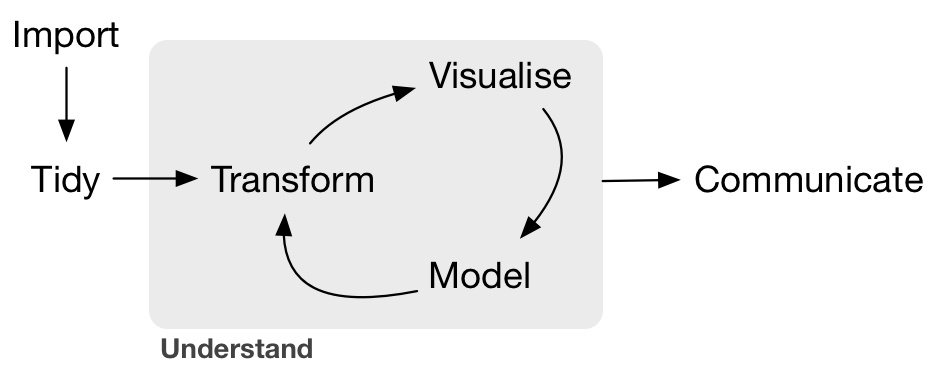
\includegraphics{./img/r4ds_data-science.png} \href{}{R for Data
Science}

\hypertarget{there-are-concepts-theory-and-tools-for-thinking-about-and-working-with-data}{%
\subsection{There are concepts, theory, and tools for thinking about and
working with
data}\label{there-are-concepts-theory-and-tools-for-thinking-about-and-working-with-data}}

Just like a field chemistry has concepts for things like moleculte,
theory for how they work, and tools for studying them, so does data
science --- for data.

\hypertarget{emphasis-on-communication}{%
\subsection{Emphasis on communication}\label{emphasis-on-communication}}

It is incredible what is possible on the communication front. Watch this
one-minute video called \href{https://vimeo.com/178485416}{What is
RMarkdown?} to blow your mind.

\hypertarget{not-just-for-big-data-or-ai-or-machine-learning}{%
\subsection{Not just for ``big data'' or AI or machine
learning}\label{not-just-for-big-data-or-ai-or-machine-learning}}

You can use data science theory and tools no matter the size or context
of your data.

\hypertarget{your-study-system-is-not-unique-when-it-comes-to-data}{%
\subsection{Your study system is not unique when it comes to
data}\label{your-study-system-is-not-unique-when-it-comes-to-data}}

Think about your data separately from your study system. Don't confound
them or it will be really hard to ask for help.

Expect there is a way to do what you want to do.

This will help you find commonalities and unite you with other lab
members and beyond.

\hypertarget{distinguish-data-questions-from-research-questions-learn-how-to-ask-for-help}{%
\subsection{Distinguish data questions from research questions, learn
how to ask for
help}\label{distinguish-data-questions-from-research-questions-learn-how-to-ask-for-help}}

\hypertarget{open-data-science-tools-exist}{%
\section{Open data science tools
exist}\label{open-data-science-tools-exist}}

\hypertarget{tools-to-match-data-science-theory}{%
\subsection{Tools to match data science
theory}\label{tools-to-match-data-science-theory}}

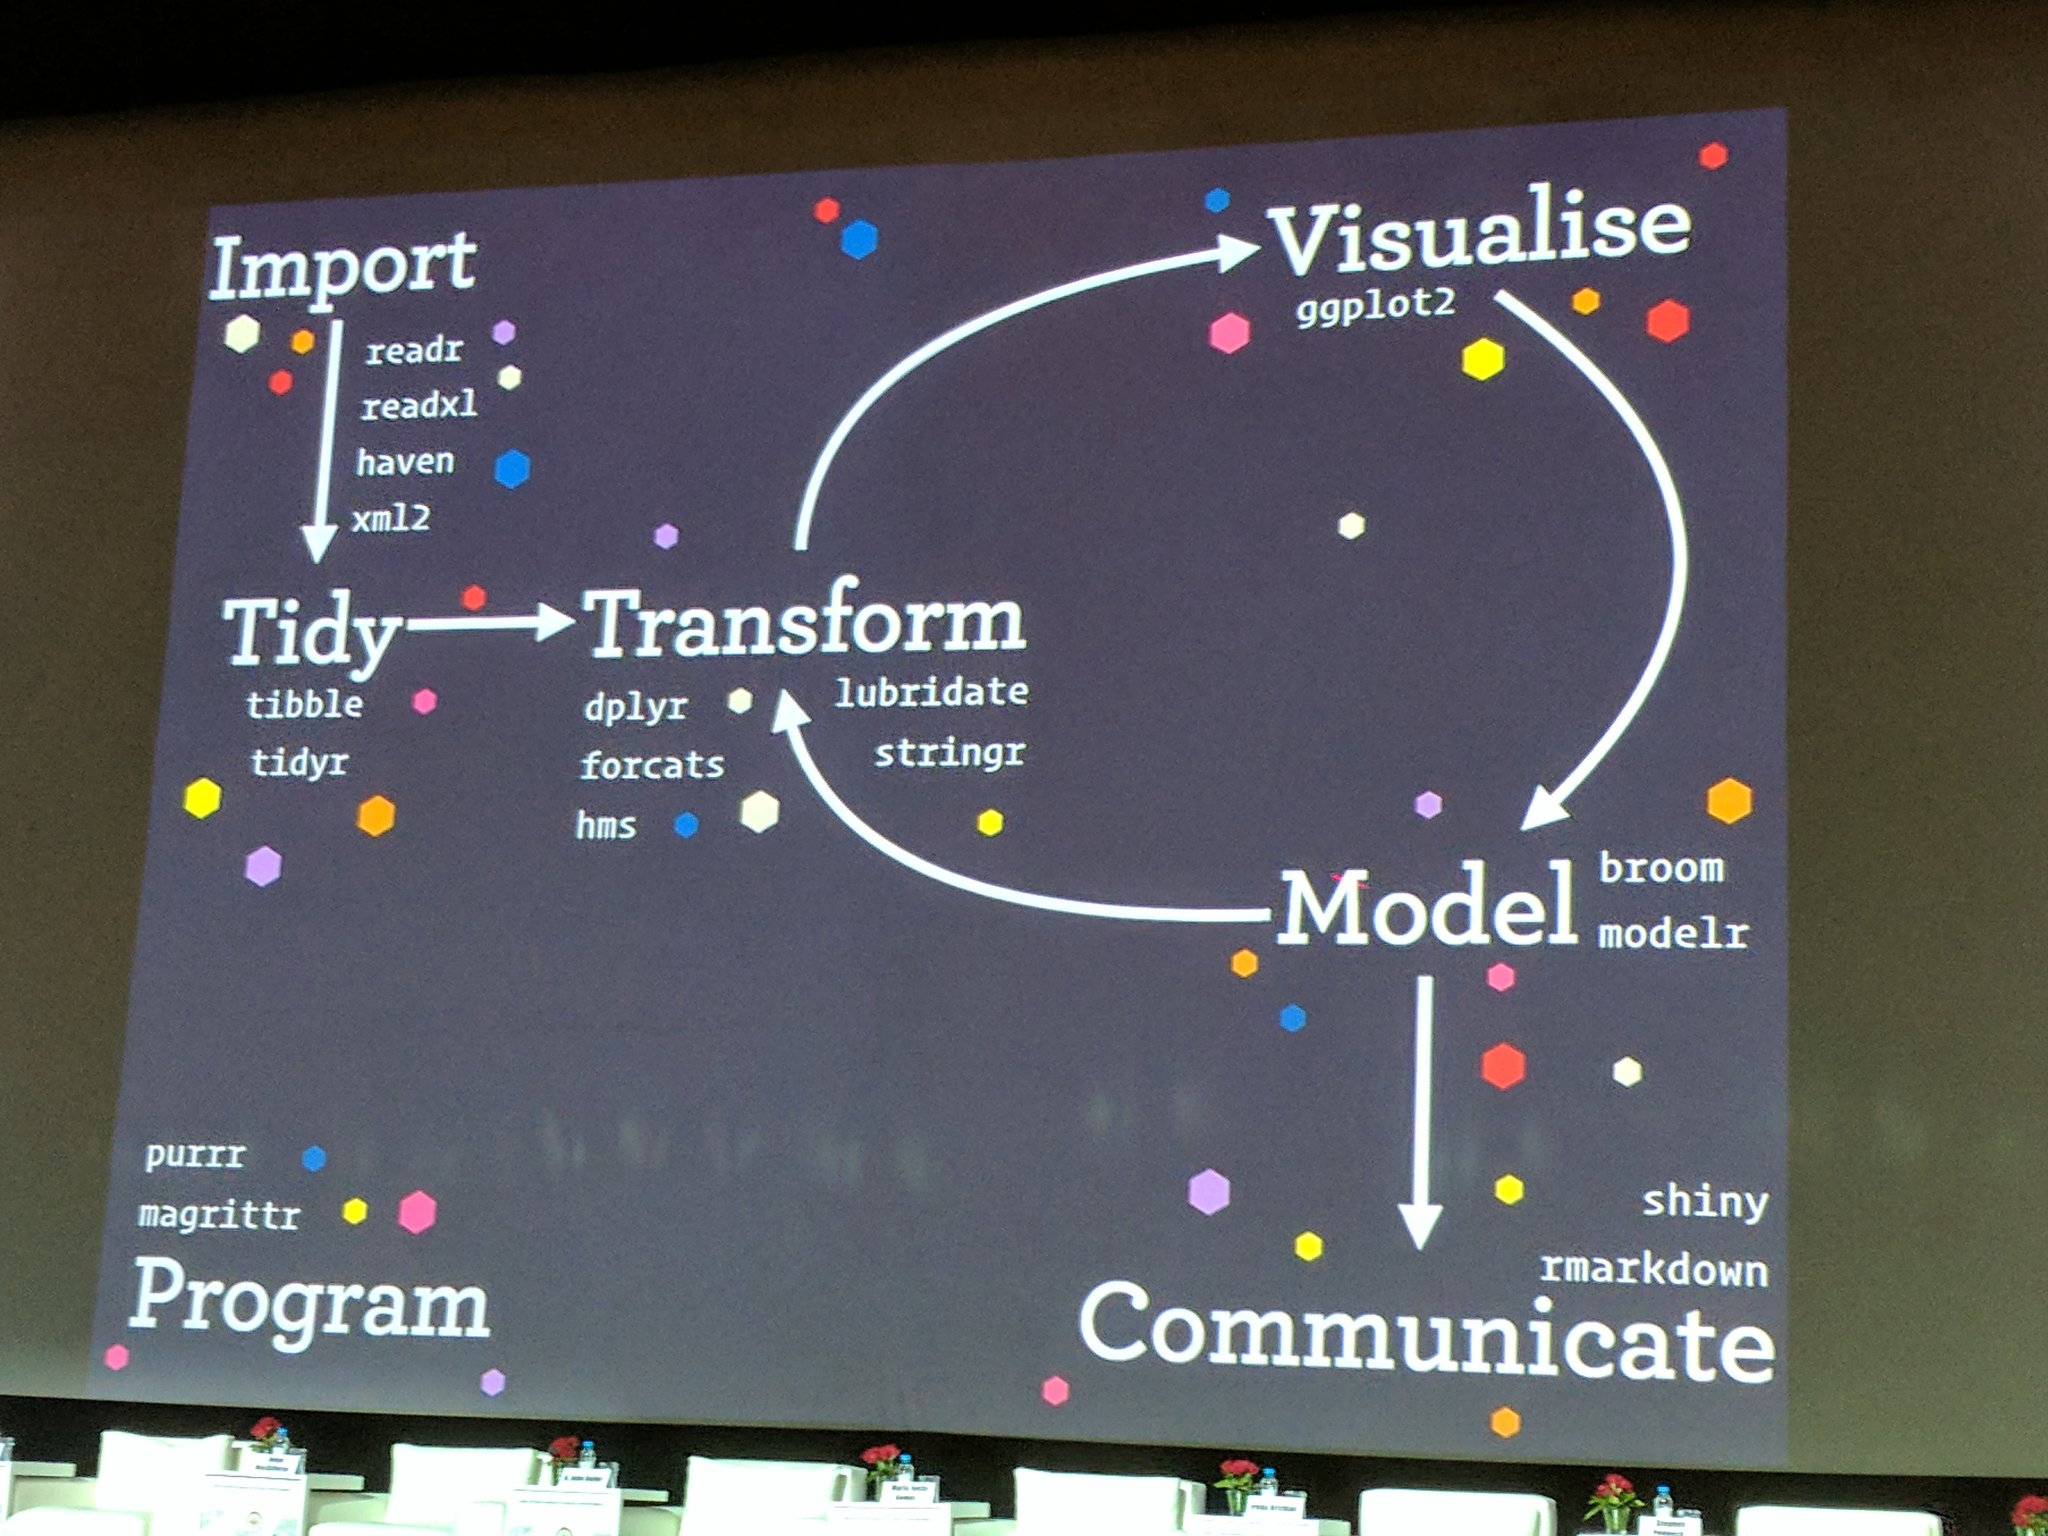
\includegraphics{./img/tidyverse_wickham_pres.jpg}

\href{}{Wickham 2017}

\hypertarget{they-exist-to-streamline-working-with-data}{%
\subsection{They exist to streamline working with
data}\label{they-exist-to-streamline-working-with-data}}

\hypertarget{and-they-are-developed-by-actual-people-nice-people}{%
\subsection{And they are developed by actual people -- nice
people!}\label{and-they-are-developed-by-actual-people-nice-people}}

\hypertarget{my-advice}{%
\subsection{My advice}\label{my-advice}}

\hypertarget{expect-there-is-a-better-way}{%
\subsubsection{Expect there is a better
way}\label{expect-there-is-a-better-way}}

If you're making the same plot 10 times, stop.

Don't confound data science with your science. Expect that someone has
had your problem before or done what you want to do.

\hypertarget{divorce-your-science-question-from-the-data-science-question}{%
\subsubsection{Divorce your science question from the data science
question}\label{divorce-your-science-question-from-the-data-science-question}}

Focus on the operations for the data, not your hypothesis

\hypertarget{google-your-question-ask-for-help}{%
\subsubsection{Google your question (ask for
help)}\label{google-your-question-ask-for-help}}

Articulate it, and identify useful solutions Trusted urls, recent dates

\hypertarget{open-as-a-way-to-work}{%
\section{Open as a way to work}\label{open-as-a-way-to-work}}

\hypertarget{open-science-as-a-way-to-be-more-efficient-and-streamlined}{%
\subsection{Open science as a way to be more efficient and
streamlined}\label{open-science-as-a-way-to-be-more-efficient-and-streamlined}}

Not an added ask at publication to share your data

It's not only about sharing data. It's about how you work, who you
include, and the tools that you use.

\hypertarget{external-memory-personal-and-collective}{%
\subsection{External memory (personal and
collective)}\label{external-memory-personal-and-collective}}

Easier on/offboarding

\hypertarget{find-solutions-faster-learn-to-talk-about-your-data}{%
\subsection{Find solutions faster -- learn to talk about your
data}\label{find-solutions-faster-learn-to-talk-about-your-data}}

\hypertarget{build-confidence-skills-are-transferable-beyond-your-science}{%
\subsection{Build confidence -- skills are transferable beyond your
science}\label{build-confidence-skills-are-transferable-beyond-your-science}}

\hypertarget{be-empathic-and-inclusive-grow-a-network-of-allies}{%
\subsection{Be empathic and inclusive -- grow a network of
allies}\label{be-empathic-and-inclusive-grow-a-network-of-allies}}

\hypertarget{lab-members-as-a-team}{%
\section{Lab members as a team}\label{lab-members-as-a-team}}

Science is collaborative. Not heads down elbows out.

\hypertarget{focus-on-what-unites-lab-members-not-what-sets-them-apart}{%
\subsection{Focus on what unites lab members, not what sets them
apart}\label{focus-on-what-unites-lab-members-not-what-sets-them-apart}}

\hypertarget{think-of-the-lab-horizontally-as-skillsets-needs-instead-of-vertically-as-science-bins}{%
\subsection{Think of the lab horizontally as skillsets \& needs instead
of vertically as science
bins}\label{think-of-the-lab-horizontally-as-skillsets-needs-instead-of-vertically-as-science-bins}}

Instead of the skills you have when you come to the lab determining how
you will be able to Do Science, have shared practices in the lab and
paths to onboard new people to work that way as well.

\hypertarget{learn-with-collaborators-and-community-redefined}{%
\section{Learn with collaborators and community
(redefined)}\label{learn-with-collaborators-and-community-redefined}}

Communities for learning, teaching, and mentorship.

\hypertarget{helps-overcome-isolation-self-taught-bad-practices-apprehension}{%
\subsection{Helps overcome isolation, self-taught bad practices,
apprehension}\label{helps-overcome-isolation-self-taught-bad-practices-apprehension}}

Stevens et al.~2018 \#\#\# Your most important collaborator is Future
You

Cannot emphasize this enough. Work now so that you can succeed later
(whether that's this afternoon or 4 years from now)

\hypertarget{communities-beyond-the-colleagues-in-your-field}{%
\subsection{Communities beyond the colleagues in your
field}\label{communities-beyond-the-colleagues-in-your-field}}

\hypertarget{learn-from-with-for-others}{%
\subsection{Learn from, with, \& for
others}\label{learn-from-with-for-others}}

\hypertarget{the-internet-as-an-underleveraged-tool-for-science}{%
\section{The internet as an underleveraged tool for
science}\label{the-internet-as-an-underleveraged-tool-for-science}}

\hypertarget{twitter-for-learning}{%
\subsection{Twitter for learning}\label{twitter-for-learning}}

Follow selectively, listen \& learn (e.g.~\#rstats)

\hypertarget{additional-reading-1}{%
\section{Additional reading}\label{additional-reading-1}}

\begin{itemize}
\tightlist
\item
  \href{https://docs.google.com/presentation/d/1INTsli9obj3BiV8xDwJc4IovPnt2EUFNyLYyF_GK7bE/present\#slide=id.g8dabbda190_0_898}{Biased
  by default: exploring discrimination in research code} - Abby Cabunoc
  Mayes Bioinformatics Community Confference Keynote 2020
\end{itemize}

\hypertarget{bsilt}{%
\chapter{Better science in less time}\label{bsilt}}

Better science is less time is science that is more efficient,
reproducible, open, inclusive, and kind. There are growing examples of
better science in less time in environmental and Earth science, and
beyond. Here are a few examples to showcase what is possible and being
done by the community.

\textbf{Slides} that have been presented during Champions Program Cohort
Calls:

\begin{itemize}
\tightlist
\item
  \href{https://docs.google.com/presentation/d/1GmuTa1sUO_boH-2TonC875pD5xvXaIMHRKIoO3vUrdY/edit?usp=sharing}{Better
  science in less time}
\item
  \href{https://docs.google.com/presentation/d/1SUMiQg0HhD19H-D6DDzTrFQVzub0kOINwJBG59uQCTw/edit\#slide=id.p1}{Empowering
  transformational science} -
  \href{https://twitter.com/ChelleGentemann}{Dr.~Chelle Gentemann}
\end{itemize}

Here we also introduce the
\href{https://drive.google.com/open?id=1X_-qPdWDCpw2F3nZr6vZnq87guyUIGLvekm0XV2H-A8}{\textbf{Pathway
document}} that teams will develop throughout the Champions program. The
Pathway is based on Table 1 in Lowndes et al.~2017, and helps teams
deliberately identify data workflow practices and next steps to
facilitate efficiency and open culture in terms of reproduciblity,
collaboration, communication, and culture.

\begin{center}\rule{0.5\linewidth}{0.5pt}\end{center}

\hypertarget{ocean-health-index-behind-the-scenes}{%
\section{Ocean Health Index: behind the
scenes}\label{ocean-health-index-behind-the-scenes}}

Some key points to discuss from
\href{https://www.nature.com/articles/s41559-017-0160}{Lowndes \emph{et
al.~2017, Nature Ecology \& Evolution}: Our path to better science in
less time using open data science tools}:

\begin{itemize}
\tightlist
\item
  Reproducibility \& communication enabled by open tooling
\item
  Shared practices are useful beyond shared projects
\end{itemize}

If you're interested in more overview of the OHI setup, see this 2017
talk (25 mins): \href{https://www.youtube.com/watch?v=x4uzVAZvFCA}{OHI
Better science in less time}

\hypertarget{ohi-pathway}{%
\subsection{OHI pathway}\label{ohi-pathway}}

\begin{itemize}
\tightlist
\item
  Motivated by necessity
\item
  Reimagined by possibility and community
\item
  Done incrementally!
\item
  Yes: it's an investment.
\item
  Also yes: huge, enduring payoff for (your) science
\end{itemize}

\hypertarget{reproducibility-communication-enabled-by-open-tooling}{%
\subsection{Reproducibility \& communication enabled by open
tooling}\label{reproducibility-communication-enabled-by-open-tooling}}

RMarkdown to reimagine data analysis and communication. RMarkdown
combines analyses \& figures together, rendered to your reporting output
of choice.

An example: \url{http://ohi-science.org/betterscienceinlesstime/}

\begin{itemize}
\tightlist
\item
  Website built with R/RMarkdown \& Github\\
\item
  You can get started too:
  (\href{https://jules32.github.io/rmarkdown-website-tutorial/}{1-hour
  tutorial})
\end{itemize}

\hypertarget{shared-workflows-not-only-useful-for-shared-projects}{%
\subsection{Shared workflows not only useful for shared
projects}\label{shared-workflows-not-only-useful-for-shared-projects}}

\begin{itemize}
\tightlist
\item
  OHI team: we identified as a team \& prioritized helping each other

  \begin{itemize}
  \tightlist
  \item
    We work on many different projects
  \item
    Use same workflows, share feedback, can think together across
    projects
  \end{itemize}
\item
  Shared conventions reduce friction \& cognitive load

  \begin{itemize}
  \tightlist
  \item
    Common ground, easier to talk about, easier to ask for help
  \item
    You don't need to design everything from scratch
  \end{itemize}
\end{itemize}

And, critically:

\begin{itemize}
\tightlist
\item
  It's about increasing efficiency and reproducibility and open science.
\item
  But it is also about increasing participation and inclusion.
\item
  Consider diversity, equity, and inclusion in your daily practices.
\item
  How you work and onboard others to your projects is a DEI issue.
\end{itemize}

\hypertarget{examples-in-the-wild-environmental-science}{%
\section{Examples in the wild: environmental
science}\label{examples-in-the-wild-environmental-science}}

\begin{itemize}
\tightlist
\item
  \href{https://stephhazlitt.github.io/regime-shifts/slides\#1}{Regime
  Shifts in R \& Data Science within the BC Public Service Observations
  from the field} - Stephanie Hazlitt, Government of British Columbia,
  slides from CascadiaRconf keynote
\item
  \href{https://github.com/EmilyMarkowitz-NOAA/NMFSReports/blob/main/presentations/2021-06-05\%20NMFSReports\%20-\%20R\%20Cascadia\%20Conf.pdf}{NMFSReports:
  Easily write NOAA reports and tech memos in R Markdown!} - Emily
  Markowitz, NOAA Alaska Fisheries Science Center, slides from
  CascadiaRconf talk
\item
  \href{https://www.openscapes.org/blog/2020/11/16/tampa-bay-reporting/}{Automated
  reporting in Tampa Bay with open science} - Marcus Beck, Tampa Bay
  Estuary Program, Openscapes blog

  \begin{itemize}
  \tightlist
  \item
    \href{https://tbep-tech.github.io/data-management-sop/workflow.html}{TBEP's
    Data Management Workflow} and open science cake
  \end{itemize}
\end{itemize}

\hypertarget{further-resources}{%
\section{Further resources}\label{further-resources}}

\hypertarget{not-so-standard-deviation-podcast}{%
\subsection{Not so standard deviation
podcast}\label{not-so-standard-deviation-podcast}}

Parker \& Peng\\
\url{http://nssdeviations.com}\strut \\
Great discussions about data concepts and ``in the wild''\\
\href{http://nssdeviations.com/episode-9-spreadsheet-drama}{Episode 9:
Spreadsheet drama}

\hypertarget{practical-computing-for-biologists}{%
\subsection{Practical computing for
biologists}\label{practical-computing-for-biologists}}

Haddock \& Dunn\\
\url{http://practicalcomputing.org/}\strut \\
Software \& computing concepts already on your computer\\
Chapter 2: Regular expressions

\hypertarget{team-culture}{%
\chapter{Team culture}\label{team-culture}}

We discuss team culture because while we know that
\href{https://www.scientificamerican.com/article/how-diversity-makes-us-smarter/}{diverse
teams are more innovative}, creating spaces where everyone can do their
best work and feel safe to contribute takes intention; it does not
happen by default. There is a lot of work to do to improve research
culture, and we can lead by example in our own research groups and
communities.

\textbf{Slides} that have been presented during Champions Program Cohort
Calls:

\begin{itemize}
\tightlist
\item
  \href{https://docs.google.com/presentation/d/1QlzV7wjP20GoLwpwUmEfBb_y4AuZnJgU_foI564FhXo/edit?usp=sharing}{Team
  culture}
\item
  \href{https://docs.google.com/presentation/d/1TwCyf9xicLWBfPhW9HnYQH3-mHycEyVKTm38zSg4D3Q/edit?usp=sharing}{Psychological
  safety}, contributed by \href{https://tararobertson.ca/}{Tara
  Robertson}
\end{itemize}

See also the following chapter on
\protect\hyperlink{code-of-conduct}{Codes of Conduct}.

\begin{center}\rule{0.5\linewidth}{0.5pt}\end{center}

\hypertarget{why-talk-about-team-culture}{%
\section{Why talk about team
culture?}\label{why-talk-about-team-culture}}

Role modeling sets a lot of team culture, and there is a lot we can
learn and do to deliberately create a scientific culture that we want to
be a part of.

\hypertarget{science-benefits-from-diversity}{%
\subsection{Science benefits from
diversity}\label{science-benefits-from-diversity}}

And we need to be deliberate about welcoming and including people from
diverse backgrounds.

A few recent articles from Nature with many more links within:

\begin{itemize}
\tightlist
\item
  \href{https://www.nature.com/articles/d41586-018-05326-3}{Science
  benefits from diversity}
\item
  \href{https://www.nature.com/articles/d41586-018-05317-4}{What does it
  take to make an institution more diverse?}
\end{itemize}

\hypertarget{sexual-harassment-is-rife-in-the-sciences}{%
\subsection{Sexual harassment is rife in the
sciences}\label{sexual-harassment-is-rife-in-the-sciences}}

\href{https://www.nature.com/articles/d41586-018-05404-6}{Sexual
harassment is rife in the sciences, finds landmark US study}.
\emph{Existing policies to address the issue are ineffective, concludes
a long-awaited report from the National Academies of Sciences,
Engineering, and Medicine.}

Most common form is gender harassment: it's the ``put-downs as opposed
to come-ons''.

\hypertarget{we-need-to-unlearn-racism-and-build-antiracist-culture-in-science}{%
\subsection{We need to unlearn racism and build antiracist culture in
science}\label{we-need-to-unlearn-racism-and-build-antiracist-culture-in-science}}

\begin{itemize}
\tightlist
\item
  \href{https://journals.plos.org/ploscompbiol/article?id=10.1371/journal.pcbi.1008210}{Ten
  simple rules for building an antiracist lab} - Chaudhary \& Berhe,
  2020. PLOS
\item
  \href{https://urgeoscience.org/}{Unlearning Racism in Geoscience ---
  URGE}
\end{itemize}

\hypertarget{put-your-values-forward}{%
\subsection{Put your values forward}\label{put-your-values-forward}}

Model the behavior you want to see in your research group \& beyond
(lab, dept, campus, organization, online)

\hypertarget{building-trust}{%
\subsection{Building trust}\label{building-trust}}

Have to build trust and be intentional, don't hope for organic.

\begin{itemize}
\tightlist
\item
  \href{https://www.ted.com/talks/frances_frei_how_to_build_and_rebuild_trust?language=en}{How
  to build (and rebuild trust} - Frances Frei
\end{itemize}

\hypertarget{sustain-the-culture}{%
\subsection{Sustain the culture}\label{sustain-the-culture}}

Overtly showing kindness \& a Code of Conduct can filter out people who
don't want to be subject to its enforcement --
\href{https://ropensci.org/blog/2016/12/21/commcallv12-review-coc/}{rOpenSci}

Labs have people coming and going all the time; how do you set the tone
and have it be sustainable?

\hypertarget{deliberately-setting-the-tone}{%
\section{Deliberately setting the
tone}\label{deliberately-setting-the-tone}}

Opening remarks at RStudio::conf 2019, in front of an audience of 1700
at a global software conference, Chief Scientist Hadley Wickham
announces the Code of Conduct, how to identify RStudio staff if you need
help, and how to mingle with welcoming body posture to invite others to
join. This set the tone of the whole conference to be the most positive
I have ever attended.

\hypertarget{collegiality}{%
\subsection{Collegiality}\label{collegiality}}

We must deliberately set the tone for collegiality to create a positive,
inclusive research group environment.

Safety and accessibility as parts of inclusion and empowerment. Does
everyone feel safe to speak up? Does everyone have channels to
contribute? This is especially true as the tech we use evolves. Who can
participate?

This builds resilience to your research group. If someone needs to leave
for a family emergency, maternity/paternity leave, vacation, set
yourselves up so your team continue smoothly/ --- Angela Bassa RStudio
talk

Opportunity cost of not doing this. Burnout, people leaving science.

\hypertarget{team-efficiency}{%
\subsection{Team efficiency}\label{team-efficiency}}

We must deliberately set the tone to create a positive, inclusive
research group environment that fuels team efficiency.

This means create a team mindset, and focusing on similarities rather
differences. We all work on different projects and have different
research questions, but we all have to wrangle data, organize version
files, have things we don't know\ldots let's create a space where we can
talk about all this and find common ground to tackle together so we
don't reinvent.

There can be an advantage to having team conventions. This can both
reduce friction and reinventing the wheel. But there also needs to be
room for different skills people come in with. For example, if they're
more efficient in Python, don't want to force R. But want to create
space where folks can interoperate and work together. The tech/software
side helps with this, but it's our mindsets too. We need to be open to
it.

\hypertarget{open-software-can-facilitate-openshared-culture}{%
\section{Open software can facilitate open/shared
culture}\label{open-software-can-facilitate-openshared-culture}}

A lot to say here, for now, see:

\begin{itemize}
\tightlist
\item
  \url{https://openscapes.github.io/slides/betterscience/environment-canada}
\item
  \url{https://blogs.scientificamerican.com/observations/open-software-means-kinder-science/}
\end{itemize}

\hypertarget{enabling-participating}{%
\section{Enabling \& participating}\label{enabling-participating}}

Here are some ideas that you can support and participate in to learn and
create a kinder team culture:

\hypertarget{seaside-chats-discuss-share-data-workflows}{%
\subsection{Seaside chats -- discuss share data
workflows}\label{seaside-chats-discuss-share-data-workflows}}

From Michelle Stuart's
\href{http://pinsky.marine.rutgers.edu/fishbowl-chat-1/}{blog about the
Pinsky Lab's first Fishbowl chat}:

\begin{quote}
This open communication has leaked into the general discussion going on
in our open work space. Lab members seem more comfortable with asking
teammates for help, and it is exciting to see all of us getting on the
same page with our data science.''�
\end{quote}

\hypertarget{hackathons-or-documentation-parties-co-create}{%
\subsection{Hackathons or documentation parties --
co-create}\label{hackathons-or-documentation-parties-co-create}}

\hypertarget{social-events}{%
\subsection{Social events}\label{social-events}}

Get to know each other outside of work. Do some during work hours can
include more people who can't participate after work

\hypertarget{onboarding-how-to-welcome-new-people-to-your-research-group}{%
\subsection{Onboarding -- how to welcome new people to your research
group}\label{onboarding-how-to-welcome-new-people-to-your-research-group}}

\hypertarget{asking-for-help}{%
\subsection{Asking for help}\label{asking-for-help}}

Create a welcoming environment where they know where to ask for help --
They won't know what questions to ask. Provide structure.

\hypertarget{code-of-conduct-next-chapter}{%
\subsection{Code of Conduct (next
chapter)!}\label{code-of-conduct-next-chapter}}

\hypertarget{further-resources-1}{%
\section{Further Resources}\label{further-resources-1}}

\begin{itemize}
\tightlist
\item
  \href{https://conversations.vanguardstem.com/a-practical-guide-to-mentoring-across-intersections-c596496ee334}{A
  Practical Guide to Mentoring Across Intersections} - Harriot 2020
  \emph{VanguardSTEM Blog}
\item
  \href{https://www.linkedin.com/pulse/get-wrong-me-what-i-need-from-allies-megan-carpenter/?trackingId=XxaMtahqr9ZJfAGcCptmFQ\%3D\%3D}{Get
  it wrong for me: What I need from allies} - Carpenter 2020.

  \begin{itemize}
  \tightlist
  \item
    ``Now, when someone asks, `what do you need from me', I say, `I need
    you to learn, I need you to care'. Somehow, we've all evolved to
    underestimate the power of learning and the power of seeking to
    understand. Knowing what things harm me is a sign that you value me.
    \ldots Then I want an ally who works to change their individual
    behavior and change the system around us for the better. Not just
    one or the other. I want a bunch of people who are interested in
    becoming allies to me to get it wrong. Because I promise, you will
    get it wrong, likely more than once. But please get it wrong, for
    me. Be wrong on my behalf. Try stuff, learn stuff, make attempts,
    and fail. Embrace the discomfort of not knowing, of not being
    certain, of not understanding and then be motivated enough to learn
    and get better. I will give you grace if you give me effort. We are
    risking our lives; you can risk getting things wrong.''
  \end{itemize}
\item
  \href{https://www.youtube.com/watch?v=AcGJ_Ldkjps}{Inclusivity in
  STEM: Interview with Dr Mica Estrada} (video, 17 mins). ``Dr.~Mica
  Estrada is a social psychologist and faculty member at University of
  San Francisco. Her research explores the role of identity and values
  in influencing the persistence of historically underserved students in
  STEM.''

  \begin{itemize}
  \tightlist
  \item
    PEERS
  \item
    micro affirmations
  \end{itemize}
\item
  \href{https://www.nature.com/articles/s41559-020-1266-7}{Recreating
  Wakanda by promoting Black excellence in ecology and evolution} ---
  Schell et al (2020)
\item
  \href{www.linkedin.com/pulse/get-wrong-me-what-i-need-from-allies-megan-carpenter}{Get
  it wrong for me: What I need from allies} --- Carpenter (2020)
\item
  \href{https://conversations.vanguardstem.com/a-practical-guide-to-mentoring-across-intersections-c596496ee334}{A
  Practical Guide to Mentoring Across Intersections} --- Harriot (2020)
\item
  \href{https://sojo.net/articles/our-white-friends-desiring-be-allies}{For
  Our White Friends Desiring to Be Allies} --- Ariel (2017)\\
\item
  \href{www.youtube.com/watch?v=oaesVb7O38s}{Dr.~Dori Tunstall on
  Respectful Design: Models for Diversity, Inclusion, \& Decolonization}
  --- Tunstall (2020)
\item
  \href{www.nature.com/articles/d41586-018-05404-6}{Sexual harassment is
  rife in the sciences, finds landmark US study} --- Witze (2018)
\item
  \href{www.allwecansave.earth}{All We Can Save} --- Johnson \&
  Wilkerson (2020)
\item
  \href{https://milkweed.org/book/braiding-sweetgrass}{Braiding
  Sweetgrass} --- Kimmerer (2013)
\end{itemize}

\hypertarget{code-of-conduct}{%
\chapter{Code of Conduct}\label{code-of-conduct}}

\emph{Please see accompanying
\href{https://docs.google.com/presentation/d/1eydm6NcrR_T2NwoMWYBWM682OW-qr755iYemVWL8cJg/edit?usp=sharing}{slides}
until this chapter is built out more.}

Please also refer to Openscapes' Code of Conduct:
\url{https://openscapes.org/code-of-conduct}

Important for:

\begin{itemize}
\tightlist
\item
  Conferences \& workshops\\
\item
  Online communities\\
\item
  Labs \& departments
\end{itemize}

\hypertarget{code-of-conduct-also-known-as}{%
\section{Code of Conduct also known
as}\label{code-of-conduct-also-known-as}}

Community Participation Guidelines\\
Code of Practice

Similar ideas:\\
Lab philosophy, mission statement, participation agreements

\hypertarget{requirements}{%
\section{Requirements}\label{requirements}}

\begin{itemize}
\tightlist
\item
  Clear explicit statements
\item
  Seen and heard -- that all participants know about

  \begin{itemize}
  \tightlist
  \item
    Accessible and discoverable online
  \item
    Mentioned aloud in meetings/interviews/onboarding
  \end{itemize}
\item
  Avenues for action, identified committees, recusals
\end{itemize}

\hypertarget{case-study-ropensci}{%
\section{Case study: rOpenSci}\label{case-study-ropensci}}

\href{https://ropensci.org/code-of-conduct/}{CoC itself}\\
\href{https://ropensci.org/blog/2019/01/14/conduct/}{Blog post about the
CoC}\\
\href{https://ropensci.org/blog/2016/12/21/commcallv12-review-coc/}{Blog
post about creating the CoC} --- following a community call on the
topic. Interesting points:

\begin{itemize}
\tightlist
\item
  Drafting -- make it good and revisit; but not a living doc
\item
  Adopting and sharing -- so people know it exists \& where to find it
\item
  Reporting and enforcing -- standardized form can help
\end{itemize}

\hypertarget{examples-to-build-from}{%
\section{Examples to build from}\label{examples-to-build-from}}

\begin{itemize}
\tightlist
\item
  \href{https://ropensci.org/code-of-conduct/}{rOpenSci CoC}\\
\item
  \href{https://open.buffer.com/code-of-conduct/}{Buffer's CoC \& Why
  It's Important For Diversity And Inclusion}
\item
  \href{https://www.mozilla.org/en-US/about/governance/policies/participation/}{Mozilla
  Community Participation Guidelines}
\item
  \href{https://github.com/dasaderi/Lab_CoC_templates/blob/master/CODE_OF_CONDUCT.md}{Template
  CoC for labs}
\end{itemize}

\hypertarget{further-reading}{%
\section{Further Reading}\label{further-reading}}

\begin{itemize}
\tightlist
\item
  \href{https://eyeondesign.aiga.org/are-codes-of-conduct-changing-the-diversity-stats-in-open-source/}{How
  Codes of Conduct Are Combatting Open Source's Diversity Problem} ---
  Margaret Rhodes, AIGA Eye on Design
\end{itemize}

\hypertarget{data-strategies}{%
\chapter{Data strategies for future us}\label{data-strategies}}

Data strategies are part of a shared workflow strategy: How do we
structure data, where do we store and back up data, how do we create
metadata, and keep the raw data raw\ldots Here we will discuss personal
and team habits for data management and sharing: data strategies for
future us.

\textbf{Slides} that have been presented during Champions Program Cohort
Calls (with guest teachers indicated):

\begin{itemize}
\tightlist
\item
  \href{https://docs.google.com/presentation/d/1rv-JfJeuYhogxV6Dpn_hNDm09nfKnOMtmZpgcciI_98/edit?usp=sharing}{Data
  strategies for Future Us}, also presented by
  \href{https://twitter.com/_ileanaf}{Ileana Fenwick}

  \begin{itemize}
  \tightlist
  \item
    \href{https://docs.google.com/presentation/d/145TOlLGH3qbJzPWdEJ2KS1LFdvP3MLTWgORHktb2R1k/edit\#slide=id.p}{Data
    stategies including data management plans (DMPs)}
  \end{itemize}
\item
  \href{https://docs.google.com/presentation/d/10X5i9zZ0uVeEaTW6F2aSvkrcxLCgW0JU9rVZvPB1ZKc/edit\#slide=id.g6532ff24f4_0_0}{Metadata},
  contributed by \href{https://www.jessicalcouture.com/}{Dr.~Jessica
  Couture}
\item
  \href{https://docs.google.com/presentation/d/12Jru3DReVH3sO-nG0msAjCNS8PVNuaYSxHi-Bxlkr1E/edit?usp=sharing}{Data
  to Product Workflows}, contributed by
  \href{https://twitter.com/emilyhmarkowitz}{Dr.~Emily Markowitz}
  (\href{https://www.youtube.com/watch?v=CyqOjQwQLy8}{video})
\end{itemize}

\begin{center}\rule{0.5\linewidth}{0.5pt}\end{center}

\hypertarget{data-organization-in-spreadsheets}{%
\section{Data organization in
spreadsheets}\label{data-organization-in-spreadsheets}}

This publication by \href{https://peerj.com/preprints/3183/}{Broman \&
Woo, 2018} appears in the ``Practical Data Science for Stats''
collection in
\href{https://peerj.com/collections/50-practicaldatascistats/}{PeerJ} \&
\href{https://www.tandfonline.com/toc/utas20/72/1}{American
Statistician}.

It is a delightful read, from the first opening sentences:

\begin{quote}
``Spreadsheets, for all of their mundane rectangularness, have been the
subject of angst and controversy for decades.\ldots{} Amid this debate,
spreadsheets have continued to play a significant role in researchers'
workflows. The dangers of spreadsheets are real, however -- so much so
that the European Spreadsheet Risks Interest Group keeps a public
archive of spreadsheet `horror stories'\ldots{}''
\end{quote}

Broman \& Woo share practical tips to make spreadsheets less
error-prone, easier for computers to process, and easier to share. And
something incredibly cool, it's the 3rd most downloaded stats paper in
the American Statistician, behind 2 papers about p-values
(\href{https://twitter.com/kwbroman/status/1326678636649394176}{twitter
thread}).

Read their paper for strategies behind their basic principles:

\begin{enumerate}
\def\labelenumi{\arabic{enumi}.}
\tightlist
\item
  Be consistent
\item
  Write dates like YYYY-MM-DD
\item
  Don't leave any cells empty
\item
  Put just one thing in a cell
\item
  Organize data as a rectangle (``Tidy data'')
\item
  Create a data dictionary
\item
  Don't include calculations in the raw data files
\item
  Don't use font color or highlighting as data
\item
  Choose good names for things
\item
  Make backups
\item
  Use data validation to avoid data entry errors
\item
  Save the data in plain text files
\end{enumerate}

\hypertarget{good-enough-practices-in-scientific-computing.}{%
\section{Good enough practices in scientific
computing.}\label{good-enough-practices-in-scientific-computing.}}

This publication by
\href{https://journals.plos.org/ploscompbiol/article?id=10.1371/journal.pcbi.1005510}{Wilson
et al.~2017} in PLoS Computational Biology follows a previous
publication by
\href{https://journals.plos.org/plosbiology/article?id=10.1371/journal.pbio.1001745}{Wilson
et al.~2014: Best practices for scientific computing}.

In terms of data management recommendataion, they have 2 main themes:

\begin{enumerate}
\def\labelenumi{\arabic{enumi}.}
\tightlist
\item
  work towards ready-to-analyze data incrementally, documenting both the
  intermediate data and the process
\item
  embrace the idea of ``tidy data'', which can be a powerful accelerator
  for analysis
\end{enumerate}

Read their paper for strategies behind their basic principles (Box 1):

\begin{enumerate}
\def\labelenumi{\arabic{enumi}.}
\tightlist
\item
  Save the raw data.
\item
  Ensure that raw data are backed up in more than one location.
\item
  Create the data you wish to see in the world.
\item
  Create analysis-friendly data.
\item
  Record all the steps used to process data.
\item
  Anticipate the need to use multiple tables, \& use a unique identifier
  for every record.
\item
  Submit data to a reputable DOI-issuing repository so that others can
  access \& cite.
\end{enumerate}

The publication also covers:

\begin{itemize}
\tightlist
\item
  Software: write, organize, and share scripts and programs used in an
  analysis.
\item
  Collaboration: make it easy for existing and new collaborators to
  understand \& contribute to a project.
\item
  Project organization: organize the digital artifacts of a project to
  ease discovery \& understanding.
\item
  Tracking changes: record how various components of your project change
  over time.
\item
  Manuscripts: write manuscripts in a way that leaves an audit trail \&
  minimizes manual merging of conflicts.
\end{itemize}

\hypertarget{make-scientific-data-fair}{%
\section{Make scientific data FAIR}\label{make-scientific-data-fair}}

This publication by
\href{https://www.nature.com/articles/d41586-019-01720-7}{Stall et al
2019} in \emph{Nature}, says that all disciplines should follow the
geosciences and demand best practice for publishing and sharing data.

FAIR data means:

\begin{itemize}
\tightlist
\item
  `Findable' by anyone using common search tools
\item
  `Accessible' so that the data and metadata can be examined
\item
  `Interoperable' so that comparable data can be analysed and integrated
  through the use of common vocabulary and formats
\item
  `Reusable' by others through robust metadata, provenance, usage
  licences
\end{itemize}

\begin{quote}
``Changes in geosciences policy and practice elevate data to valuable
research contributions rather than files that are shoved in as an
afterthought.''
\end{quote}

Read their paper for strategies and examples behind changing the
culture: There are three big changes are crucial to shift research
culture across all disciplines:

\begin{enumerate}
\def\labelenumi{\arabic{enumi}.}
\tightlist
\item
  Make depositing open and FAIR data a priority for all.
\item
  Recognize and incentivize FAIR data practices.
\item
  Fund global infrastructure to support FAIR data and tools.
\end{enumerate}

\hypertarget{tidy-data-for-efficiency-reproducibility-collaboration}{%
\section{Tidy data for efficiency, reproducibility, \&
collaboration}\label{tidy-data-for-efficiency-reproducibility-collaboration}}

By \href{https://www.openscapes.org/blog/2020/10/12/tidy-data/}{Lowndes
\& Horst 2020}, posted on the Openscapes blog: an illustrated series to
tell a story about tidy data.

Tidy data has been mentioned in each of the above, as a way to organize
data in spreadsheets, to prepare ready-to-analyze data, and for sharing
with the FAIR principles.

So what is tidy data?

First, a preamble:

\begin{itemize}
\tightlist
\item
  Raw data may not be stored in a tidy way
\item
  ``Wrangling'' data into tidy structure should be done programmatically
  as part of the analytical process - keep the raw data raw
\item
  Tidy data is a philosophy
\item
  There are existing tools to help
\end{itemize}

Remember that ``tidying data (``data wrangling'') -- up to 50--80\% of a
data scientist's time''
\href{https://www.nytimes.com/2014/08/18/technology/for-big-data-scientists-hurdle-to-insights-is-janitor-work.html}{Lohr
2014, New York Times}, so it's important to leverage these existing
philosophies and tools.

When we talk about organizing data to help us work in an efficient,
reproducible, and collaborative way, we are talking about TIDY DATA. We
mean deliberately thinking about the shape and structure of data --
something that might not seem super exciting but is truly game-changing.

So let's talk about what tidy data is and why it is so empowering for
your analytical life.

\hypertarget{what-is-tidy-data}{%
\subsection{What is tidy data?}\label{what-is-tidy-data}}

Tidy data is a way to describe data that's organized with a particular
structure -- a rectangular structure, where each variable has its own
column, and each observation has its own row (Wickham 2014).

This standard structure of tidy data led Hadley Wickham to describe it
the way Leo Tolstoy describes families. Leo says ``Happy families are
all alike; every unhappy family is unhappy in its own way''. Similarly,
Hadley says ``tidy datasets are all alike, but every messy dataset is
messy in its own way''.

\hypertarget{tidy-data-for-more-efficient-data-science}{%
\subsection{Tidy data for more efficient data
science}\label{tidy-data-for-more-efficient-data-science}}

Tidy data allows you to be more efficient by using existing tools
deliberately built to do the things you need to do, from subsetting
portions of your data to plotting maps of your study area. Using
existing tools saves you from building from scratch each time you work
with a new dataset (which can be time-consuming and demoralizing). And
luckily, there are a lot of tools specifically built to wrangle untidy
data into tidy data (for example, in the tidyr package). By being more
equipped to wrangle your data into a tidy format, you can get to your
analyses faster to start answering the questions you're asking.

\hypertarget{tidy-data-for-easier-collaboration}{%
\subsection{Tidy data for easier
collaboration}\label{tidy-data-for-easier-collaboration}}

Tidy data makes it easier to collaborate because our friends can use the
same tools in a familiar way. Whether thinking about collaborators as
current teammates, your future self, or future teammates, organizing and
sharing data in a consistent and predictable way means less adjustment,
time, and effort for all.

\hypertarget{tidy-data-for-reproducibility-and-reuse}{%
\subsection{Tidy data for reproducibility and
reuse}\label{tidy-data-for-reproducibility-and-reuse}}

Tidy data also makes it easier to reproduce analyses because they are
easier to understand, update, and reuse. By using tools together that
all expect tidy data as inputs, you can build and iterate really
powerful workflows. And, when you have additional data entries, it's no
problem to re-run your code!

\hypertarget{tidy-data-for-the-win}{%
\subsection{Tidy data for the win!}\label{tidy-data-for-the-win}}

Once you are empowered with tools to work with tidy data generally, it
opens up a whole new world of datasets that feel more approachable
because you can work using familiar tools. This transferrable confidence
and ability to collaborate might be the best thing about tidy data.

So for more efficient, reproducible, and collaborative analyses, make
friends with tidy data!

\begin{center}\rule{0.5\linewidth}{0.5pt}\end{center}

\hypertarget{learn-more-about-tidy-data}{%
\subsection{Learn more about tidy
data:}\label{learn-more-about-tidy-data}}

\hypertarget{further-reading-1}{%
\section{Further Reading}\label{further-reading-1}}

\begin{itemize}
\item
  Wickham, H (2014). \emph{Tidy Data}. Journal of Statistical Software
  58 (10).
  \href{http://www.jstatsoft.org/v59/i10/}{jstatsoft.org/v59/i10/}
\item
  Broman, KW and KH Woo (2018). \emph{Data Organization in
  Spreadsheets}.
  \href{https://doi.org/10.1080/00031305.2017.1375989}{The American
  Statistician 72 (1)}. Available open access as a
  \href{https://peerj.com/preprints/3183/}{PeerJ preprint}.
\item
  Grolemund, G \& Wickham, H (2016). R for Data Science: Ch 12 (Tidy
  Data) \url{https://r4ds.had.co.nz}
\item
  Leek, J (2016). \href{https://github.com/jtleek/datasharing}{How to
  share data with a statistician}
\end{itemize}

\hypertarget{coding-strategies}{%
\chapter{Coding strategies for future us}\label{coding-strategies}}

Coding strategies can blend with workflow strategies, and the idea is
working in a way that is not just for you in this moment. Here we will
discuss good coding practices for beginning and seasoned coders alike
that make it easier to work with other people, times, and computers.

\textbf{Slides} that have been presented during Champions Program Cohort
Calls (with guest teachers indicated):

\begin{itemize}
\tightlist
\item
  \href{https://docs.google.com/presentation/d/1nTLJ782dpZqp3MEhQU9zNaFInrTaFUVQbj9OqsmxUYo/edit?usp=sharing}{Coding
  strategies for future us}

  \begin{itemize}
  \tightlist
  \item
    See previous iterations:
    \href{https://docs.google.com/presentation/d/1HbxQ9Lg-ySEhmvH01PnMX0BDuquQezru73GI3PV-Ibo/edit?usp=sharing}{Filepaths}
    and
    \href{https://docs.google.com/presentation/d/1hiSjMjTFhdDO5lLCM4uiU3D8nLFPt8eOEdDPVoaG5UQ/edit?usp=sharing}{Project-oriented
    workflows}
  \end{itemize}
\item
  \href{https://docs.google.com/presentation/d/1a620vM5OkOgcUi0I-mQPV5ZTQglRfwSnAb6O41g8tv0/edit\#slide=id.p1}{Expanding
  ouR community!}, contributed by
  \href{https://twitter.com/DrFintastic}{Dr.~Chanté Davis}
\item
  \href{https://noaa-edab.github.io/presentations/20211015_Openscapes_Bastille.html}{State
  of the Ecosystem Product Development Workflow}, contributed by Kim
  Bastille
\end{itemize}

\begin{center}\rule{0.5\linewidth}{0.5pt}\end{center}

\hypertarget{software-considerations-for-coding}{%
\section{Software considerations for
coding}\label{software-considerations-for-coding}}

The following advice is from Tiffany Timbers, UBC Data Science,
\href{https://github.com/ttimbers/intro-to-reticulate/blob/main/slides/reticulate-intro.pdf}{Intro
to Reticulate}:

\textbf{You will need these software tools:}

\begin{itemize}
\tightlist
\item
  Programming language (R, python)
\item
  Code editor (RStudio IDE, Jupyter)
\item
  Version control software (git, GitHub/bitbucket)
\end{itemize}

\textbf{How to choose the ``best'' tool for the job:}

\begin{itemize}
\tightlist
\item
  Reproducible and auditable
\item
  Accurate
\item
  Collaborative (and portable)
\end{itemize}

If you're choosing between R, Python, and other modern languages, they
will aready be reproducible, auditable, and accurate. That leaves
collaboration -- what do your collaborators use? What do folks in your
lab, or field use? What is mentioned in the papers you read? There is
increasing interoperability between languages (e.g.~see
\href{https://rstudio.github.io/reticulate/}{reticulate} to run python
code from R) so when you have some idea it's best to get started!

See also: \href{https://peerj.com/preprints/3210}{Opinionated analysis
development (Parker 2017)}. Tools like RStudio are already doing this to
help you. Reserve your mental energy for the fun part of the analysis!

\hypertarget{wtf-what-they-forgot-to-teach-you}{%
\section{WTF: What They Forgot to teach
you}\label{wtf-what-they-forgot-to-teach-you}}

Most of this advice comes directly from Jenny Bryan \& Jim Hester's
awesome course \href{https://whattheyforgot.org}{What they Forgot to
Teach You About R}. I highly recommend reading Chapters 1-4 that go into
much better detail than the notes here. The advice here is solid coding
practices for any language, with examples from R.

\hypertarget{workflow-versus-product}{%
\subsection{Workflow versus product}\label{workflow-versus-product}}

Distinction between things you do because of personal taste \& habits
(``workflow'') versus the logic and output that is the essence of your
project (``product'').

\textbf{Workflow:}

\begin{itemize}
\tightlist
\item
  Editor you use to write code.
\item
  Name of your home directory.
\item
  R code you ran before lunch.
\end{itemize}

\textbf{Clearly product:} - Raw data. - R code someone needs to run on
your raw data to get your results, including the explicit library()
calls to load necessary packages. (script, notebook)

\textbf{Ideally, you don't hardwire anything about your workflow into
your product.}

\hypertarget{source-files}{%
\section{Source files}\label{source-files}}

What are they and why?

Code that creates objects is ``source code''. Source code is essentially
text files you edit in a text editor that is then executed in the
console.

Examples:

\begin{itemize}
\tightlist
\item
  .R, .Rmd
\item
  .py
\item
  .m
\end{itemize}

\hypertarget{save-the-source-not-the-workspace}{%
\subsection{Save the source, not the
workspace}\label{save-the-source-not-the-workspace}}

Save the source code; do not save the R object itself.

Save your commands as ``scripts'' (\texttt{.R}, \texttt{.py}) or
``notebooks'' (\texttt{.Rmd}, \texttt{ipynb}). It doesn't have to be
polished. Just save it!

Everything that really matters should be achieved through code that you
save -- including objects and figures The contrast is storing them
implicitly or explicitly, as part of an entire workspace, or clicking
via the mouse.

Load libraries/packages at the top. Just like a recipe: tell us the
ingredients need before we get going!

\hypertarget{always-start-r-with-a-blank-slate}{%
\subsection{Always start R with a blank
slate}\label{always-start-r-with-a-blank-slate}}

Saving code is an absolute requirement for reproducibility.

When you quit, do not save the workspace to an .Rdata file. When you
launch, do not reload the workspace from an .Rdata file.

In RStudio, set this via \emph{Tools \textgreater{} Global Options.}

\hypertarget{restart-r-often-during-development}{%
\subsection{Restart R often during
development}\label{restart-r-often-during-development}}

\begin{quote}
``Have you tried turning it off and then on again?'' -- timeless
troubleshooting wisdom, applies to everything
\end{quote}

If you use RStudio, use the menu item Session \textgreater{} Restart R

Additional ways to restart development where you left off, i.e.~``re-run
all the code up to HERE''

\hypertarget{avoid-rmlist-ls}{%
\subsection{\texorpdfstring{Avoid
\texttt{rm(list\ =\ ls())}}{Avoid rm(list = ls())}}\label{avoid-rmlist-ls}}

It's common to see scripts begin with this object-nuking command:
\texttt{rm(list\ =\ ls())}

This is highly suggestive of a non-reproducible workflow.

\textbf{The problem with \texttt{rm(list\ =\ ls())} is that, given the
intent, it does not go far enough.}

It only deletes user-created objects from the global workspace.

Instead, Restart R with a clean slate OFTEN (e.g.~many times/day), and
write every script assuming it will be run in a fresh R process

\hypertarget{filepaths}{%
\section{Filepaths}\label{filepaths}}

Every saved thing gets a unique path.

Your code needs to run from somewhere specific. And when it interacts
with other things (data or other code), you need to tell your code where
things are.

The more deliberate you are about where things live,

\begin{itemize}
\tightlist
\item
  The easier it will be for you and future you
\item
  The easier it will be for other people
\item
  The easier it will be on another computer
\end{itemize}

\hypertarget{setwdpaththatonlyworksonmymachine}{%
\subsection{setwd(``path/that/only/works/on/my/machine'')}\label{setwdpaththatonlyworksonmymachine}}

The chance of \texttt{setwd()} having the desired effect -- making the
file paths work -- for anyone besides its author is 0\%.

It's also unlikely to work for the author one or two years or computers
from now.

Hard-wired, absolute paths, especially when sprinkled throughout the
code, make a project brittle. Such code does not travel well across time
or space.

\hypertarget{setwd}{%
\subsection{setwd()}\label{setwd}}

BUT, if you still decide to use \texttt{setwd()} in your scripts, you
should at least be very disciplined about it:

Only use \texttt{setwd()} at the very start of a file, i.e.~in an
obvious and predictable place.

Always set working directory to the same thing, namely to the top-level
of the project. Always build subsequent paths relative to that.

\hypertarget{r-users-use-the-here-package}{%
\subsection{\texorpdfstring{R users: use the \texttt{here}
package}{R users: use the here package}}\label{r-users-use-the-here-package}}

\texttt{here()} identifies your project's files, based on the current
working directory at the time when the package is loaded.

\begin{verbatim}
library(here)
here()
\end{verbatim}

\hypertarget{project-oriented-workflows}{%
\section{Project oriented workflows}\label{project-oriented-workflows}}

\hypertarget{dilemma-and-solution}{%
\subsection{Dilemma and Solution}\label{dilemma-and-solution}}

\textbf{Problem statement:}

We want to work on project A with the working directory set to
path/to/projectA (my data analysis) and on project B with the working
directory set to path/to/projectB (my teaching material).

But we also want to keep code like setwd(``path/to/projectA'') out of
our scripts.

\textbf{Solution:}

Solution: use an IDE that supports a project-based workflow.

An
\href{https://en.wikipedia.org/wiki/Integrated_development_environment}{integrated
development environment} (IDE) offers:

\begin{itemize}
\tightlist
\item
  a powerful, R-aware code editor
\item
  many ways to send your code to a running R process
\item
  other modern conveniences
\end{itemize}

And it eliminates:

\begin{itemize}
\tightlist
\item
  temptation to develop code directly in the Console. (instead:.R!)
\item
  tension between development convenience and portability of the code.
\end{itemize}

\hypertarget{organize-your-work-into-projects}{%
\subsection{Organize your work into
projects}\label{organize-your-work-into-projects}}

Here's what I mean by ``work in a project'':

\begin{itemize}
\tightlist
\item
  File system discipline: put all files related to a project in a
  designated folder.

  \begin{itemize}
  \tightlist
  \item
    This applies to data, code, figures, notes, etc.
  \item
    Depending on project complexity, you might enforce further
    organization into subfolders.
  \end{itemize}
\item
  Working directory intentionality: when working on project A, make sure
  working directory is set to project A's folder.

  \begin{itemize}
  \tightlist
  \item
    Ideally, this is achieved via the development workflow and tooling,
    not by baking absolute paths into the code.
  \end{itemize}
\item
  File path discipline: all paths are relative --- relative to the
  project's folder.
\end{itemize}

Synergistic habits: you'll get the biggest payoff if you practice all of
them together.

Portability: the project can be moved around on your computer or onto
other computers and will still ``just work''. is the only practical
convention that creates reliable, polite behavior across different
computers/users/time. This convention is neither new, nor unique to R.

It's like agreeing that we will all drive on the left or the right. A
hallmark of civilization is following conventions that constrain your
behavior a little, in the name of public safety.

\hypertarget{rstudio-projects}{%
\subsection{RStudio Projects}\label{rstudio-projects}}

The RStudio IDE has a notion of a (capital ``P'') Project, which is a
very effective implementation of (small ``p'') projects.

Project have an.Rproj file in the folder, which is used to store
settings specific to that project. Use File \textgreater{} New Project
\ldots{} to get started.

Allows for multiple projects

no danger of crosstalk: each has own R process, global workspace \&
working directory

Same ``unit'' as a GitHub repo!

\hypertarget{tips-for-rstudio-projects}{%
\subsection{Tips for RStudio Projects}\label{tips-for-rstudio-projects}}

One suggestion for organizing:

Have a dedicated folder for your Projects. - If you have One Main Place
for Projects, then go there in Finder/File Explorer to launch any
specific project with .Rproj. - Mine is called
``\textasciitilde/github/''.

Switching Projects: RStudio knows about recent Projects.

\hypertarget{name-files-deliberately}{%
\subsection{Name files deliberately}\label{name-files-deliberately}}

Jenny Bryan's 3 rules for Naming Things:

\begin{itemize}
\tightlist
\item
  machine readable
\item
  human readable
\item
  plays well with default ordering
\end{itemize}

Available from
\href{https://speakerdeck.com/jennybc/how-to-name-files}{Speakerdeck}

\hypertarget{further-reading-2}{%
\section{Further reading}\label{further-reading-2}}

\begin{itemize}
\tightlist
\item
  \href{https://jhudatascience.org/tidyversecourse/}{Tidyverse Skills
  for Data Science} - Wright, Ellis, Hicks, \& Peng
\item
  \href{https://journals.plos.org/ploscompbiol/article?id=10.1371/journal.pcbi.1008770}{Principles
  for data analysis workflows} - Stoudt, Vasquez, and Martinez 2021,
  PLOS Computational Biology
\item
  \href{https://rc2e.com/}{R Cookbook} --- JD Long
\end{itemize}

\hypertarget{communities}{%
\chapter{Open communities}\label{communities}}

Open communities play a big role in advancing research, helping research
feel less lonely and reducing the amount of time we all spend being
stuck spend reinventing the wheel. This is a brief (incomplete)
introduction to the idea of open communities. We will explore: What are
open communities? Why engage with them? How to engage with them? And
also how Twitter as a legit tool for coding and science. Originally
focusing on R communities, we are adding more examples beyond.

\textbf{Slides} that have been presented during Champions Program Cohort
Calls:

\begin{itemize}
\tightlist
\item
  \href{https://docs.google.com/presentation/d/17HSNmBYvPw-7Prioys7WIhL9QGVb3s3bJCLaAJVaChc/edit?usp=sharing}{Open
  Communities}, which we go through in a Cohort Call
\item
  \href{https://docs.google.com/presentation/d/1czvMz7a84jkaYDwHlG1cuKyf9B0mciQJVOFcc7hZtpU/edit?usp=sharing}{Discovering
  Community Tools}, which teams review during a Seaside Chat
\end{itemize}

\begin{center}\rule{0.5\linewidth}{0.5pt}\end{center}

\hypertarget{what-are-open-communities}{%
\section{What are open communities?}\label{what-are-open-communities}}

Open communities are groups of people openly creating, sharing,
teaching, collaborating. They are united around a shared interest:
coding language, topic, discipline, etc.

They have a culture of shared \& continued learning, prioritize
diversity, equity, inclusion.

They have online and in-person activities.

Here are some examples of communities. Read more \& direct links:
\url{https://rstudio-conf-2020.github.io/r-for-excel/collaborating.html\#r-communities}

Some \#rstats communities with in-person and online events and channels

There are strategies for learning with both online and local
communities.

\hypertarget{why-engage-with-open-communities}{%
\section{Why engage with open
communities?}\label{why-engage-with-open-communities}}

\begin{itemize}
\tightlist
\item
  Skillshare (teach \& learn)

  \begin{itemize}
  \tightlist
  \item
    Coding, software, workflows
  \item
    Collaboration, leadership, DEIJ
  \end{itemize}
\item
  Meet allies, grow friendships, career opportunities
\item
  Help improve science \& scientific culture

  \begin{itemize}
  \tightlist
  \item
    Increase visibility \& value of coding, data, collaboration skills
  \item
    Drive change: modern ways to contribute to science. Formally
    incentivize and teach! Include in promotion/tenure (we shouldn't
    really have to teach ourselves on our own time and not be credited),
    create jobs
  \end{itemize}
\item
  Carry on \& forward your experience from Openscapes
\end{itemize}

\hypertarget{how-to-get-started}{%
\section{How to get started?}\label{how-to-get-started}}

Google your interests/needs. When you Google, include what you want to
do PLUS r, rstats; python.

Start by listening and learning. Be deliberate: curate who you follow.

Like and share when you're comfortable.

Then, contribute -- your ideas, your blogs, your papers, your
code\ldots{} Contributors are welcome in open communities! And know too
that the R packages ggplot \& knitr were created by students (Wickham \&
Xie) (see
\href{https://resources.rstudio.com/rstudio-conf-2019/our-colour-of-magic-the-open-sourcery-of-fantastic-r-packages}{McBain
2019}).

Finally, Twitter is a legit tool for science. It's a good way to learn
what you need to learn and broadening your horizons while building
community. Some places to start:
\texttt{\#rstats,\ \#rstatsES,\ \#rspatial,\ \#pydata,\ \#BlackAndSTEM,\ \#MeTooSTEM}

\href{https://github.com/Openscapes/seaside-chats\#seaside-chats}{Seaside
Chats} are a great way to start exploring together.

\hypertarget{examples-in-the-wild-campus-coding-clubs}{%
\section{Examples in the wild: campus coding
clubs}\label{examples-in-the-wild-campus-coding-clubs}}

\begin{itemize}
\tightlist
\item
  \href{http://eco-data-science.github.io/}{EcoDataScience} at UC Santa
  Barbara
\item
  \href{https://biodata-club.github.io}{BioData Club} at OHSU
\item
  \href{https://www.biodataclub.org/}{The Bio-Data Club} at Moffitt
\end{itemize}

\hypertarget{github-pub}{%
\chapter{GitHub for Publishing}\label{github-pub}}

GitHub is a powerful tool for collaborative coding with version control,
but in the next two chapters we are going to focus on some of its
lesser-celebrated awesomeness: GitHub for publication and project
management. We will focus on how to use GitHub for collaboration and
communication for science, and spend time with hands-on practice.

\textbf{Slides} that have been presented during Champions Program Cohort
Calls:

\begin{itemize}
\tightlist
\item
  \href{https://docs.google.com/presentation/d/1PzGAbEpNhT6CDPe1DCHf5-eVAjy-2R2D3VMHz7dY774/edit?usp=sharing}{GitHub
  Clinic}
\end{itemize}

\begin{center}\rule{0.5\linewidth}{0.5pt}\end{center}

\hypertarget{preamble}{%
\section{Preamble}\label{preamble}}

We are going to work with GitHub from the browser only, because it makes
the best use of our short time together. It is also a powerful way for
folks to contribute and collaborate even if they are not involved in
day-to-day hands-on analysis. So this might be good for new lab members
or students to contribute to your lab as soon as possible.

GitHub can reduce friction for open science: it gives us avenues for
communicating and publishing methods, blogs, interactive graphics and
more, without a lot of heavy lifting!

\hypertarget{prerequisite}{%
\subsection{Prerequisite}\label{prerequisite}}

You will need to create \textbf{GitHub} account at
\url{http://github.com}, if you don't already have one. For username, I
recommend all lower-case letters, short as you can. I recommend using
your \emph{.edu email}, since you can request free private repositories
via \href{https://education.github.com/}{GitHub Education} discount.

\hypertarget{what-is-github-traditional-answer}{%
\section{What is GitHub? --- Traditional
answer}\label{what-is-github-traditional-answer}}

GitHub means GitHub.com; it's a company that is an online collaborative
platform, with some features familiar to social media users.

GitHub centers around git, which is powerful version control software
for your local computer. This has been around for years, taking care of
bookkeeping for you locally on your computer.

GitHub makes git's local bookkeeping collaborative through its powerful
online platform. It will weave together all the version control from
your local computer with other collaborators you work with.

It is used for code and files: organize, archive, bookkeeping,
searchable, changes visualized, etc. In the figure below, notice the
familiar red and green to denote deletions and additions line-by-line,
with darker shading to identify specific text within a line. Also notice
the differencing in the image's color bar!

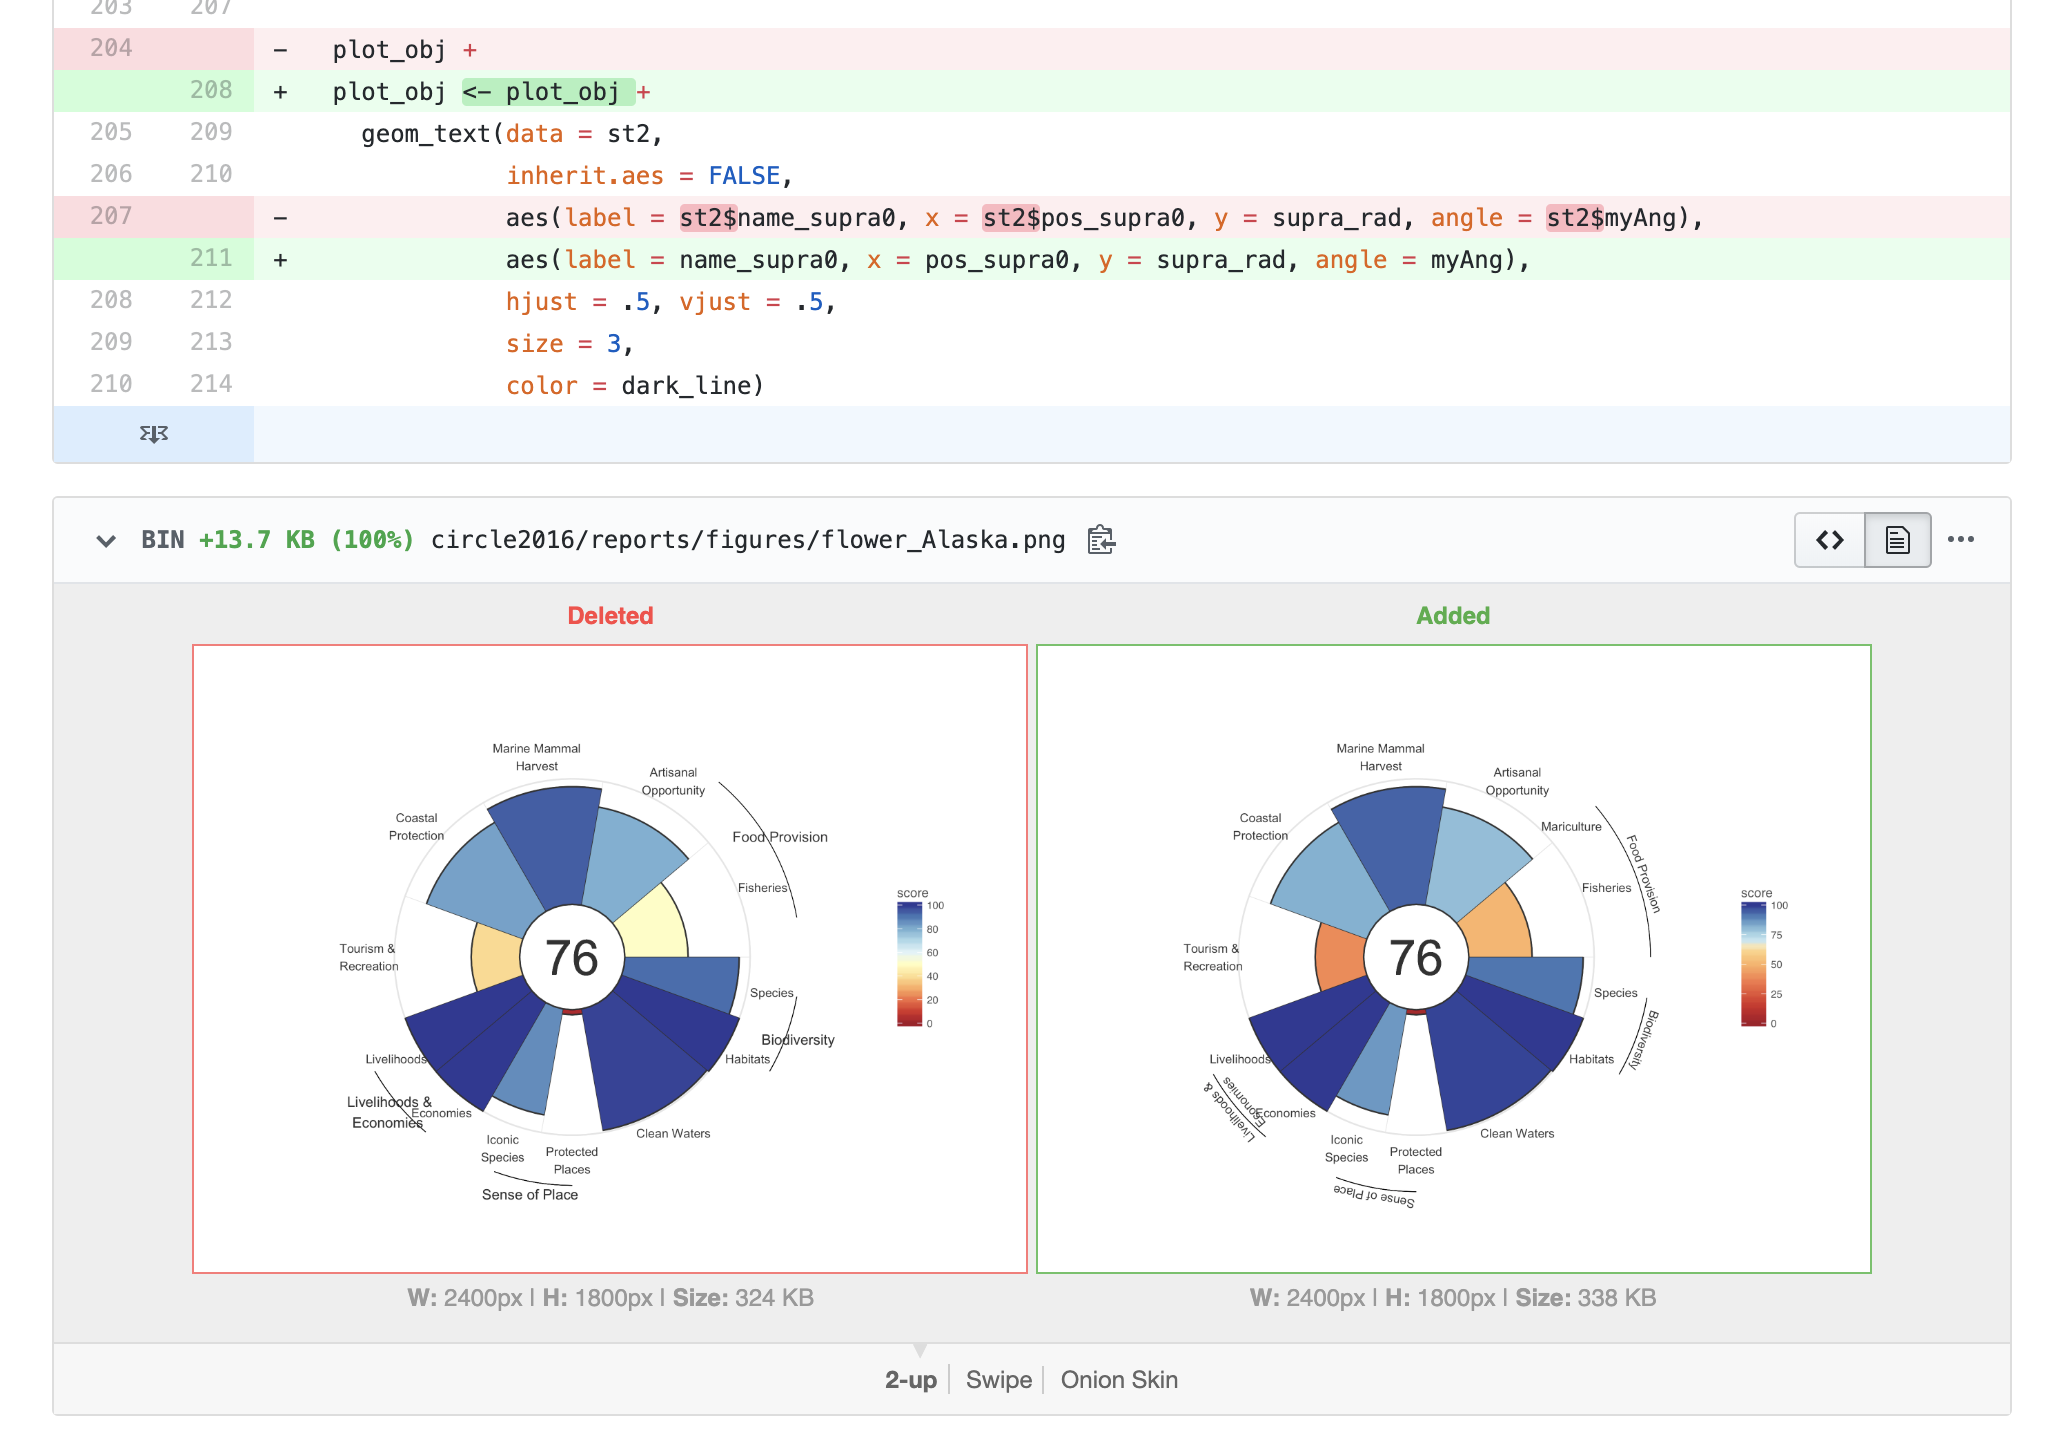
\includegraphics[width=0.8\textwidth,height=\textheight]{./img/github-differencing.png}

We aren't going to teach traditional git/GitHub today, but here are some
recommendations if you'd like to learn. First, read Jenny Bryan's
``Excuse Me, Do You Have a Moment to Talk About Version Control?''
(open-access pre-print from
\href{https://peerj.com/preprints/3159/}{PeerJ}, published in
\href{https://www.tandfonline.com/doi/full/10.1080/00031305.2017.1399928}{The
American Statistican}). This provides an excellent overview. One quote I
like in particular is

\begin{quote}
Collaboration is the most compelling reason to manage a project with Git
and GitHub. My definition of collaboration includes hands-on
participation by multiple people, including your past and future self,
as well as an asymmetric model, in which some people are active makers
and others only read or review. - \emph{Jenny Bryan, ``Excuse Me, Do You
Have a Moment to Talk About Version Control?''}
\end{quote}

Next, to learn GitHub with R, the absolute best resource is Jenny
Bryan's \href{https://happygitwithr.com/}{Happy Git With R}. This is a
comprehensive, friendly step-by-step process of how to do so, and is an
awesome reference for seasoned git/GitHub users as well. If you want a
shorter-form resource, I'd recommend 2 tutorials from
\href{http://ohi-science.org/data-science-training/}{OHI-Science's
data-science-training}. This also teaches you how to set up GitHub to
sync directly through RStudio, so that you don't have to have any other
software (including the command line) open to do so:

\begin{itemize}
\tightlist
\item
  \href{http://ohi-science.org/data-science-training/github.html}{GitHub}
\item
  \href{http://ohi-science.org/data-science-training/collaborating.html}{Collaborating
  with GitHub}
\end{itemize}

On my local computer, I interact with GitHub through RStudio 99.9\% of
the time (use command line .1\% of time). \emph{Upcoming: resources for
setting up GitHub without RStudio}

\hypertarget{what-is-github-non-traditional-answer}{%
\section{What is GitHub? --- Non-traditional
answer}\label{what-is-github-non-traditional-answer}}

\hypertarget{publishing-platform}{%
\subsection{Publishing platform}\label{publishing-platform}}

It's for books like this one
(\href{https://openscapes.org/series}{openscapes.org/series}), websites
like \href{https://openscapes.org}{openscapes.org}, which was built with
R's blogdown package, and interactive dashboards.

\hypertarget{project-management-system}{%
\subsection{Project management system}\label{project-management-system}}

GitHub is also a project management system for short and long-term
tasks. It is really powerful to have collaborative ``todo'''s in the
same software (and user accounts) as all the analysis and all the people
that you're already working with.

We will talk about ``Issues'' \& ``Projects'' in the next chapter.

\hypertarget{github-framework-in-a-nutshell}{%
\section{GitHub framework in a
nutshell}\label{github-framework-in-a-nutshell}}

\hypertarget{users-vs.-organizations}{%
\subsection{Users vs.~organizations}\label{users-vs.-organizations}}

Example: \href{https://github.com/jules32}{jules32} is a user account,
\href{https://github.com/openscapes}{openscapes} is an organization
group.

You can think of them like other social media accounts: I can be an
individual or part of a group, and there are permissions associated with
both.

\hypertarget{repositories-repos}{%
\subsection{Repositories (``repos'')}\label{repositories-repos}}

Repos are GitHub's main unit. They are essentially a folder, and you'll
put files and folders in them. They are contained, with permissions
specific to each one.

It makes it easier to navigate through and find stuff --- so you are
``not sifting through a zoo of files'' as one Openscapes Champion has
said.

\hypertarget{commits-commit-messages}{%
\subsection{``Commits'' \& ``commit
messages''}\label{commits-commit-messages}}

Unlike Dropbox or Google Drive that constantly and automatically sync to
the cloud, you have to deliberately tell git/GitHub when you have an
amount of work that you want to be versioned and synced. You have to
commit to telling them. GitHub takes care of the backend bookkeeping
involved, but you have to write a human-readable message to your future
self and others. That is the commit message.

There is no absolute guidance for how often to commit, but I think of it
as leaving breadcrumbs for yourself. How much work and on what things/in
what combination would you like to be able to reverse? What kind of
information will make it easier for Future You to work with?

\hypertarget{public-vs-private}{%
\subsection{Public vs private}\label{public-vs-private}}

You can have both public (the free default) and private repositories,
and change these permissions later on. I mostly work in public repos,
but if I work in private ones, I often have the expectation that they
will be made public some day. So I practice good habits with commits and
documentation, and keep conversations on-topic.

\hypertarget{the-search-feature-is-awesome}{%
\subsection{The search feature is
awesome}\label{the-search-feature-is-awesome}}

You are able to search within a GitHub repository, across repositories
in an organization, or across all GitHub public repositories. I find
this helps me find things quickly if I'm looking for how I've used a
function in the past, or if I remember a word that would stand out that
I included in a commit message as a breadcrumb to myself. It will also
search Issues within the repositories, so you can look for specific
words in conversations as well.

\hypertarget{branches-forks}{%
\subsection{Branches \& Forks}\label{branches-forks}}

We're not going to talk about branches and forks. These are a core
feature of what makes GitHub super powerful for software development,
and one of the first things you'll see in GitHub tutorials geared
towards software engineers. But I do not think that is the most relevant
or smoothest entryway for those of us who are scientists fairly new to
collaborative coding and version control.

\hypertarget{github-orientation}{%
\section{GitHub Orientation}\label{github-orientation}}

This is a demo \emph{details upcoming}

\begin{Shaded}
\begin{Highlighting}[]
\NormalTok{knitr}\SpecialCharTok{::}\FunctionTok{include\_graphics}\NormalTok{(}\StringTok{"img/github{-}orientation.png"}\NormalTok{)  }
\end{Highlighting}
\end{Shaded}

\begin{figure}[H]

{\centering 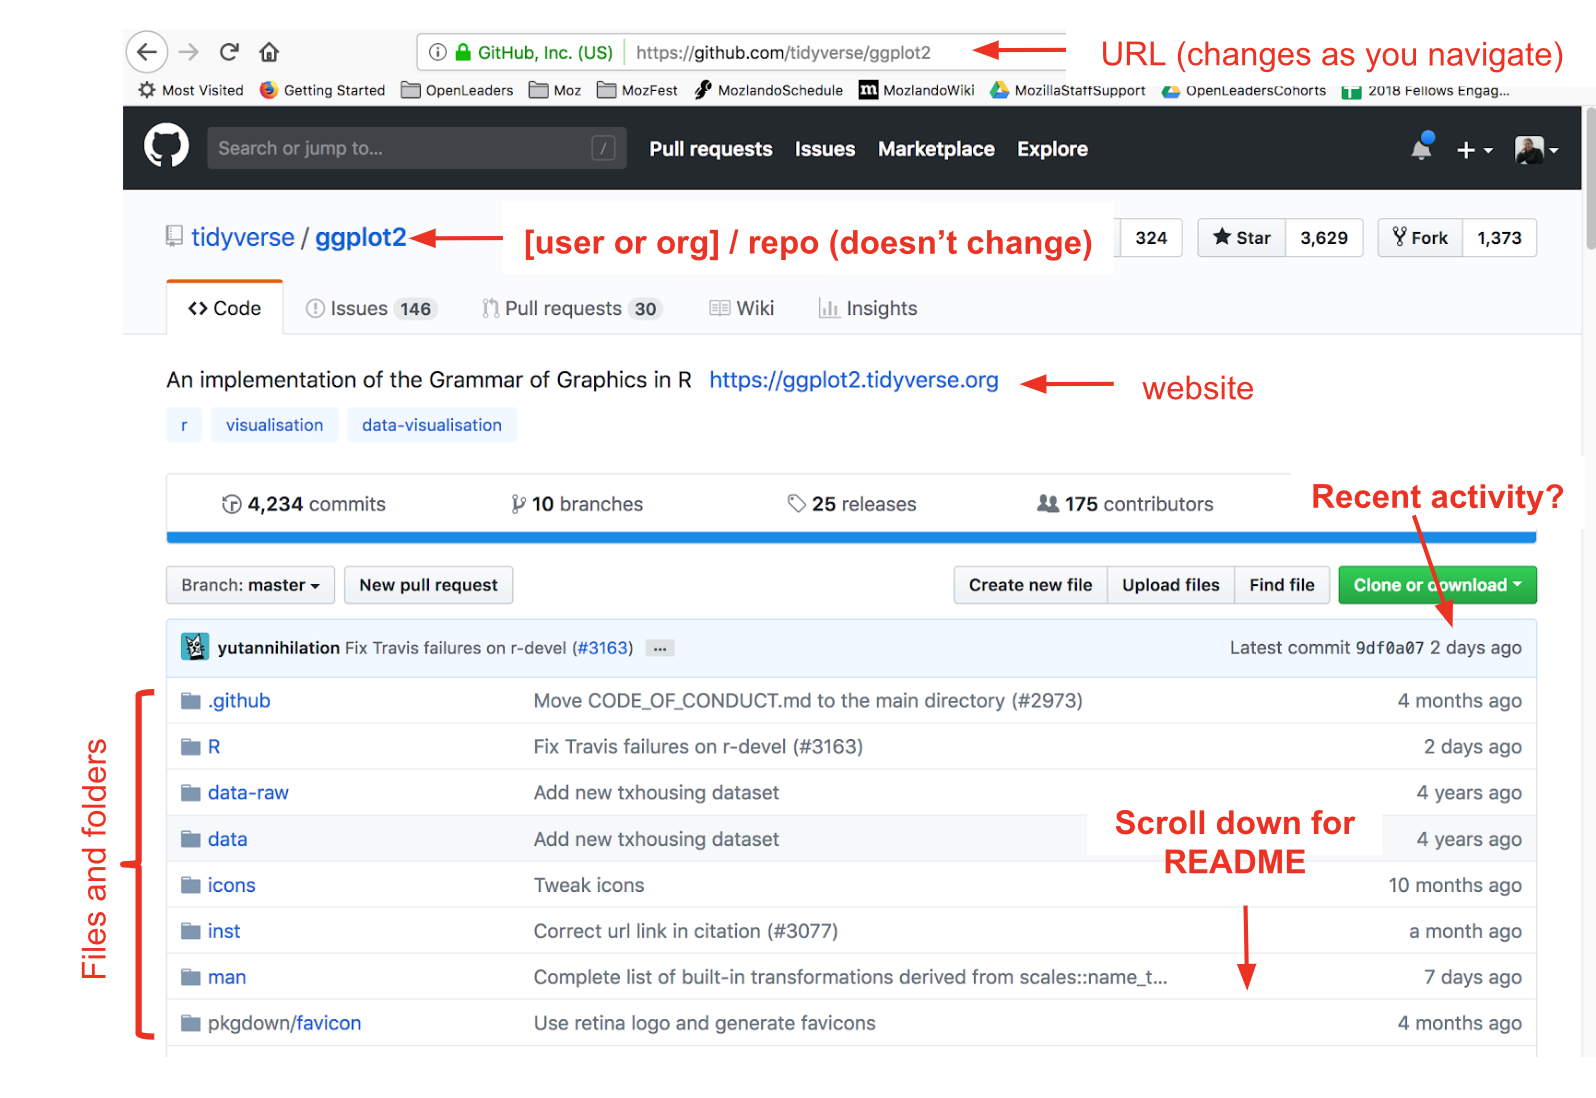
\includegraphics[width=0.8\textwidth,height=\textheight]{./img/github-orientation.png}

}

\end{figure}

\hypertarget{editing-files-from-github.}{%
\section{Editing files from GitHub.}\label{editing-files-from-github.}}

This is also a demo \emph{details upcoming}

First a Disclaimer: you don't want to edit from the browser for most
things -- you would want to ``clone'' the repo to your local computer
and leverage more goodies \& power. However, you will sometimes edit in
the browser, and it's a good entry point for us today, and maybe for
onboarding folks in your lab in the future.

Why not edit in the browser? You don't want to overwrite each other or
forget yourself. Good for quick md editing, not script editing.

In the demo, the example .md was a deliberate example of sharing slides
from a talk :)

What to do: (you all have permissions)

\begin{itemize}
\tightlist
\item
  Go to \url{https://github.com/openscapes/demo/}yourname.md
\item
  Click on the pencil to edit your file
\item
  Make many edits \& commits with commit messages

  \begin{itemize}
  \tightlist
  \item
    github.com has a default message, but get into the habit of writing
    an actual message to yourself/others (breadcrumbs)
  \end{itemize}
\item
  This is different from saving (cancel if you save!)
\end{itemize}

\hypertarget{further-resources-2}{%
\section{Further resources}\label{further-resources-2}}

\begin{itemize}
\tightlist
\item
  \href{https://www.youtube.com/watch?v=eWxxfttcMts}{Git for Humans} -
  Alice Bartlett, 2016
\end{itemize}

\hypertarget{github-issues}{%
\chapter{GitHub for Project Management}\label{github-issues}}

GitHub is best known as a collaborative coding platform. But of course
productive collaboration requires communication, and GitHub has powerful
features to support communication and project management through GitHub
Issues. (Also see thee previous chapter about GitHub for publishing).

\textbf{Slides} that have been presented during Champions Program Cohort
Calls:

\begin{itemize}
\tightlist
\item
  \href{https://docs.google.com/presentation/d/1PzGAbEpNhT6CDPe1DCHf5-eVAjy-2R2D3VMHz7dY774/edit?usp=sharing}{GitHub
  Clinic}
\end{itemize}

\begin{center}\rule{0.5\linewidth}{0.5pt}\end{center}

\hypertarget{preamble-1}{%
\section{Preamble}\label{preamble-1}}

We are focusing on GitHub Issues here because they are a powerful way
for team members to have active discussions about data and code, and
therefore ways to participate in analyses even for those that are not
involved in the day-to-day coding. I find Issues not only useful to
discuss topics as a team, but I also treat it as my external memory: I
write notes to myself, link to files and websites; I leave breadcrumbs
for myself so that I am more easily able to remember my past thought
processes and pick up projects where I left off.

In this way, GitHub Issues help actualize the mindset of \textbf{Future
You} and \textbf{Future Us}. This means being deliberate now about
communicating decisions and progress so that you or others can work in
the future a little more smoothly. Using project management software is
a strategy used by every software developer or people working on
projects with many moving parts. It streamlines technical discussions
with people who are coming/joining a group. It also helps organize and
track projects that single or multiple \& overlapping users can be a
part of.

While there are many options for project management software out there,
I like using GitHub because it's already managing my code and my work,
and linked to my collaborators so it offers a streamlined way to
communicate. It's also one less account I need to have, which is a huge
bonus in my mind.

One of the reason we talk about Issues in Openscapes is because they are
an excellent way to develop habits for using GitHub for your analytical
project more broadly.

\hypertarget{what-are-issues}{%
\section{What are Issues?}\label{what-are-issues}}

Every GitHub repository (shortened to ``repo'') has a feature called
Issues. Issues is GitHub's project management and task-tracking feature.

\begin{quote}
Issues ``track ideas, enhancements, tasks, or bugs for work on GitHub.''
- \href{https://help.github.com/en/articles/about-issues}{GitHub}
\end{quote}

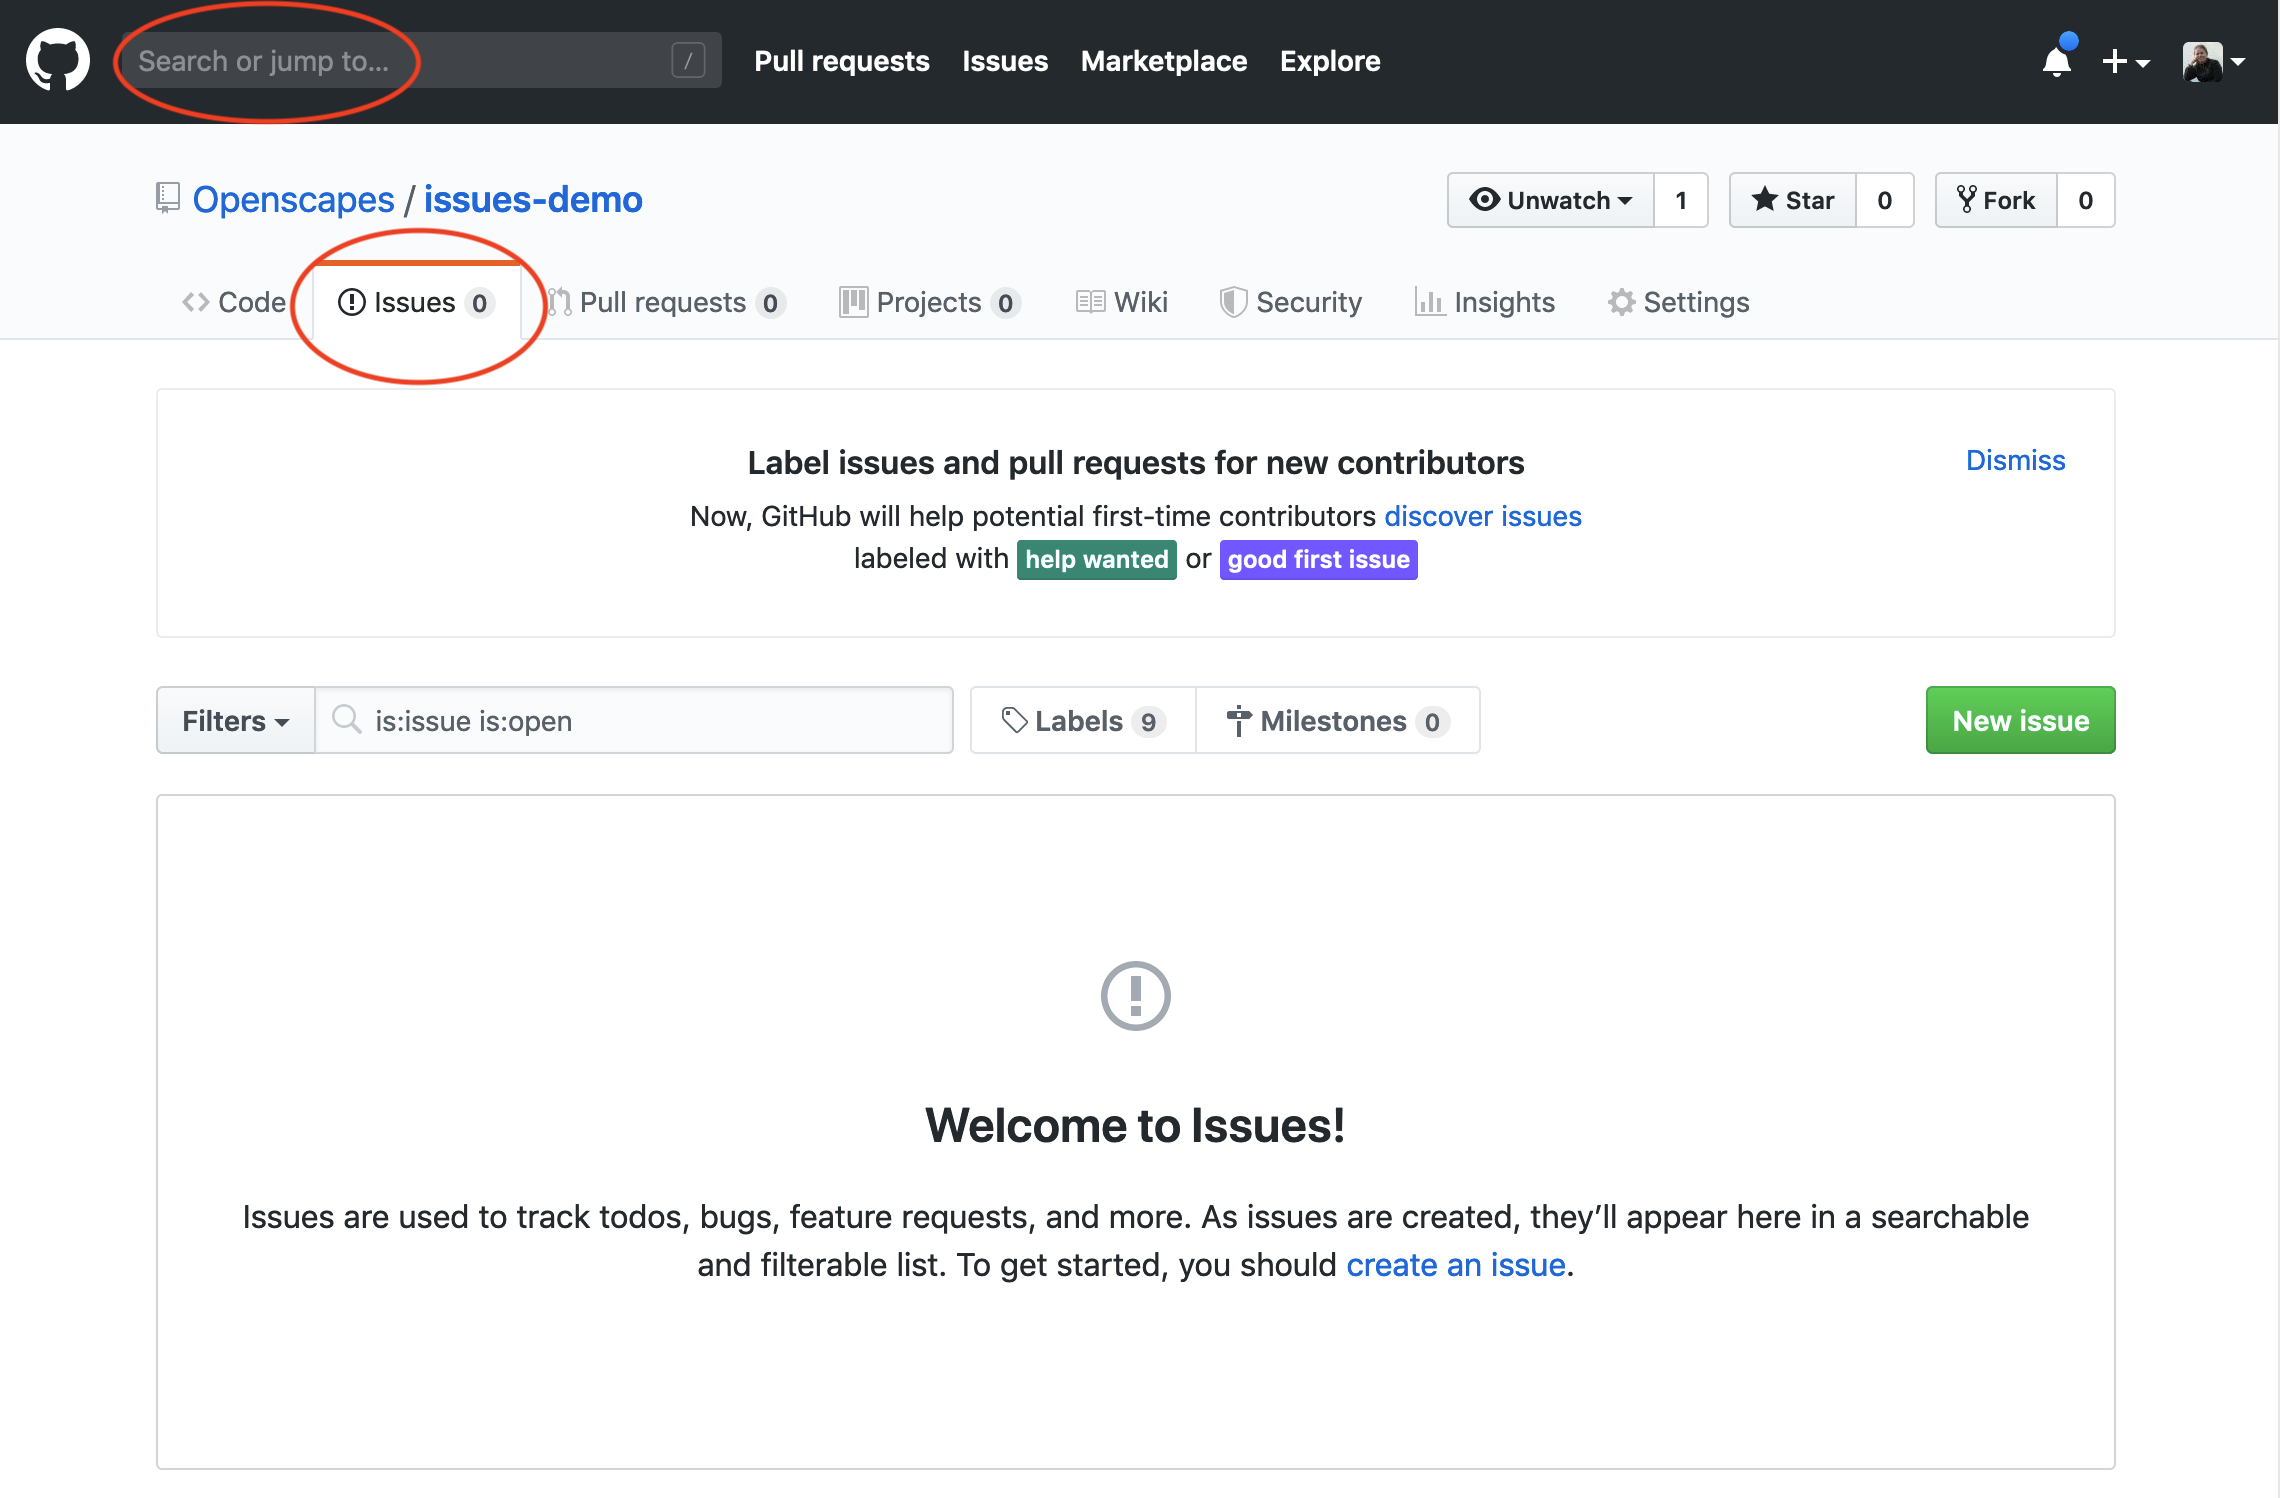
\includegraphics[width=0.8\textwidth,height=\textheight]{./img/issues-intro.png}

\href{https://twitter.com/jennybryan/}{Jenny Bryan} has an excellent
summary of Issues in her article ``Excuse Me, Do You Have a Moment to
Talk About Version Control?'' (open-access pre-print from
\href{https://peerj.com/preprints/3159/}{PeerJ}, published in
\href{https://www.tandfonline.com/doi/full/10.1080/00031305.2017.1399928}{The
American Statistican}):

\begin{quote}
GitHub issues are another powerful feature of the platform. Recall that
we are repur- posing Git, a tool that facilitates software development.
Think of the issues for a project as its bug tracker. For projects that
are not pure software development, we co-opt this machinery to organize
our to-do list more generally. The basic unit is an issue and you can
interact with one in two ways.
\end{quote}

\begin{quote}
First, issues are integrated into the project's web interface on GitHub,
with a rich set of options for linking to project files and incremental
changes. Second, issues and their associated comment threads appear in
your email, just like regular messages (this can, of course, be
configured). The result is that all correspondence about a project comes
through your normal channels, but is also tracked inside the project
itself, with excellent navigability and search capabilities. For
software, issues are used to track bugs and feature requests. In a data
analysis project, you might open an issue to flesh out a specific
sub-analysis or to develop a complicated figure. In a course, we use
them to manage homework submission, marking, and peer review.
\end{quote}

\begin{quote}
Issues can be assigned to specific people and they can be labelled,
e.g.~``bug'', ``simulation- study'', or ``final-exam''. Coupled with the
ability to cross-link issues and the project files or file changes, you
have extraordinary power to document why things have happened in the
past and to organize what needs to happen in the future.
\end{quote}

You create an Issue for a topic, and use it track progress or ask
questions. You can provide links, describe updates, link to other
Issues, and you can close the Issue when it is completed. You can also
re-open previously-closed Issues.

Every GitHub repository has this Issues feature. This means that
sometimes Issues are public and sometimes they are private.

\begin{itemize}
\tightlist
\item
  In a public repo, anyone with a GitHub username can create and comment
  on issues.
\item
  In a private repo, only users with permission can create and comment
  on issues, or see them at all
\end{itemize}

GitHub search is awesome -- it will search all of your files and Issues!

\hypertarget{issues-in-the-wild}{%
\section{Issues in the Wild}\label{issues-in-the-wild}}

Here are some examples of ``traditional'' and ``non-traditional'' use of
issues.

\href{https://github.com/tidyverse/ggplot2/issues}{ggplot2's Issues} is
an example of what I think is the ``traditional'' use of Issues, which
is in a pretty pure software development context. This is a public
repository, and all topics are directly related to ggplot2. Issues are
largely used to report bugs, troubleshoot and sometimes to request
features. Note the ``Filters'' feature on the top-left: this by default
will search through the Issues that are still open, but you can also
change this if you wanted to search also for closed Issues (just below
``Filters'' you can see that there are over 2000 closed Issues,
documenting the innovation that's been ongoing in ggplot2).

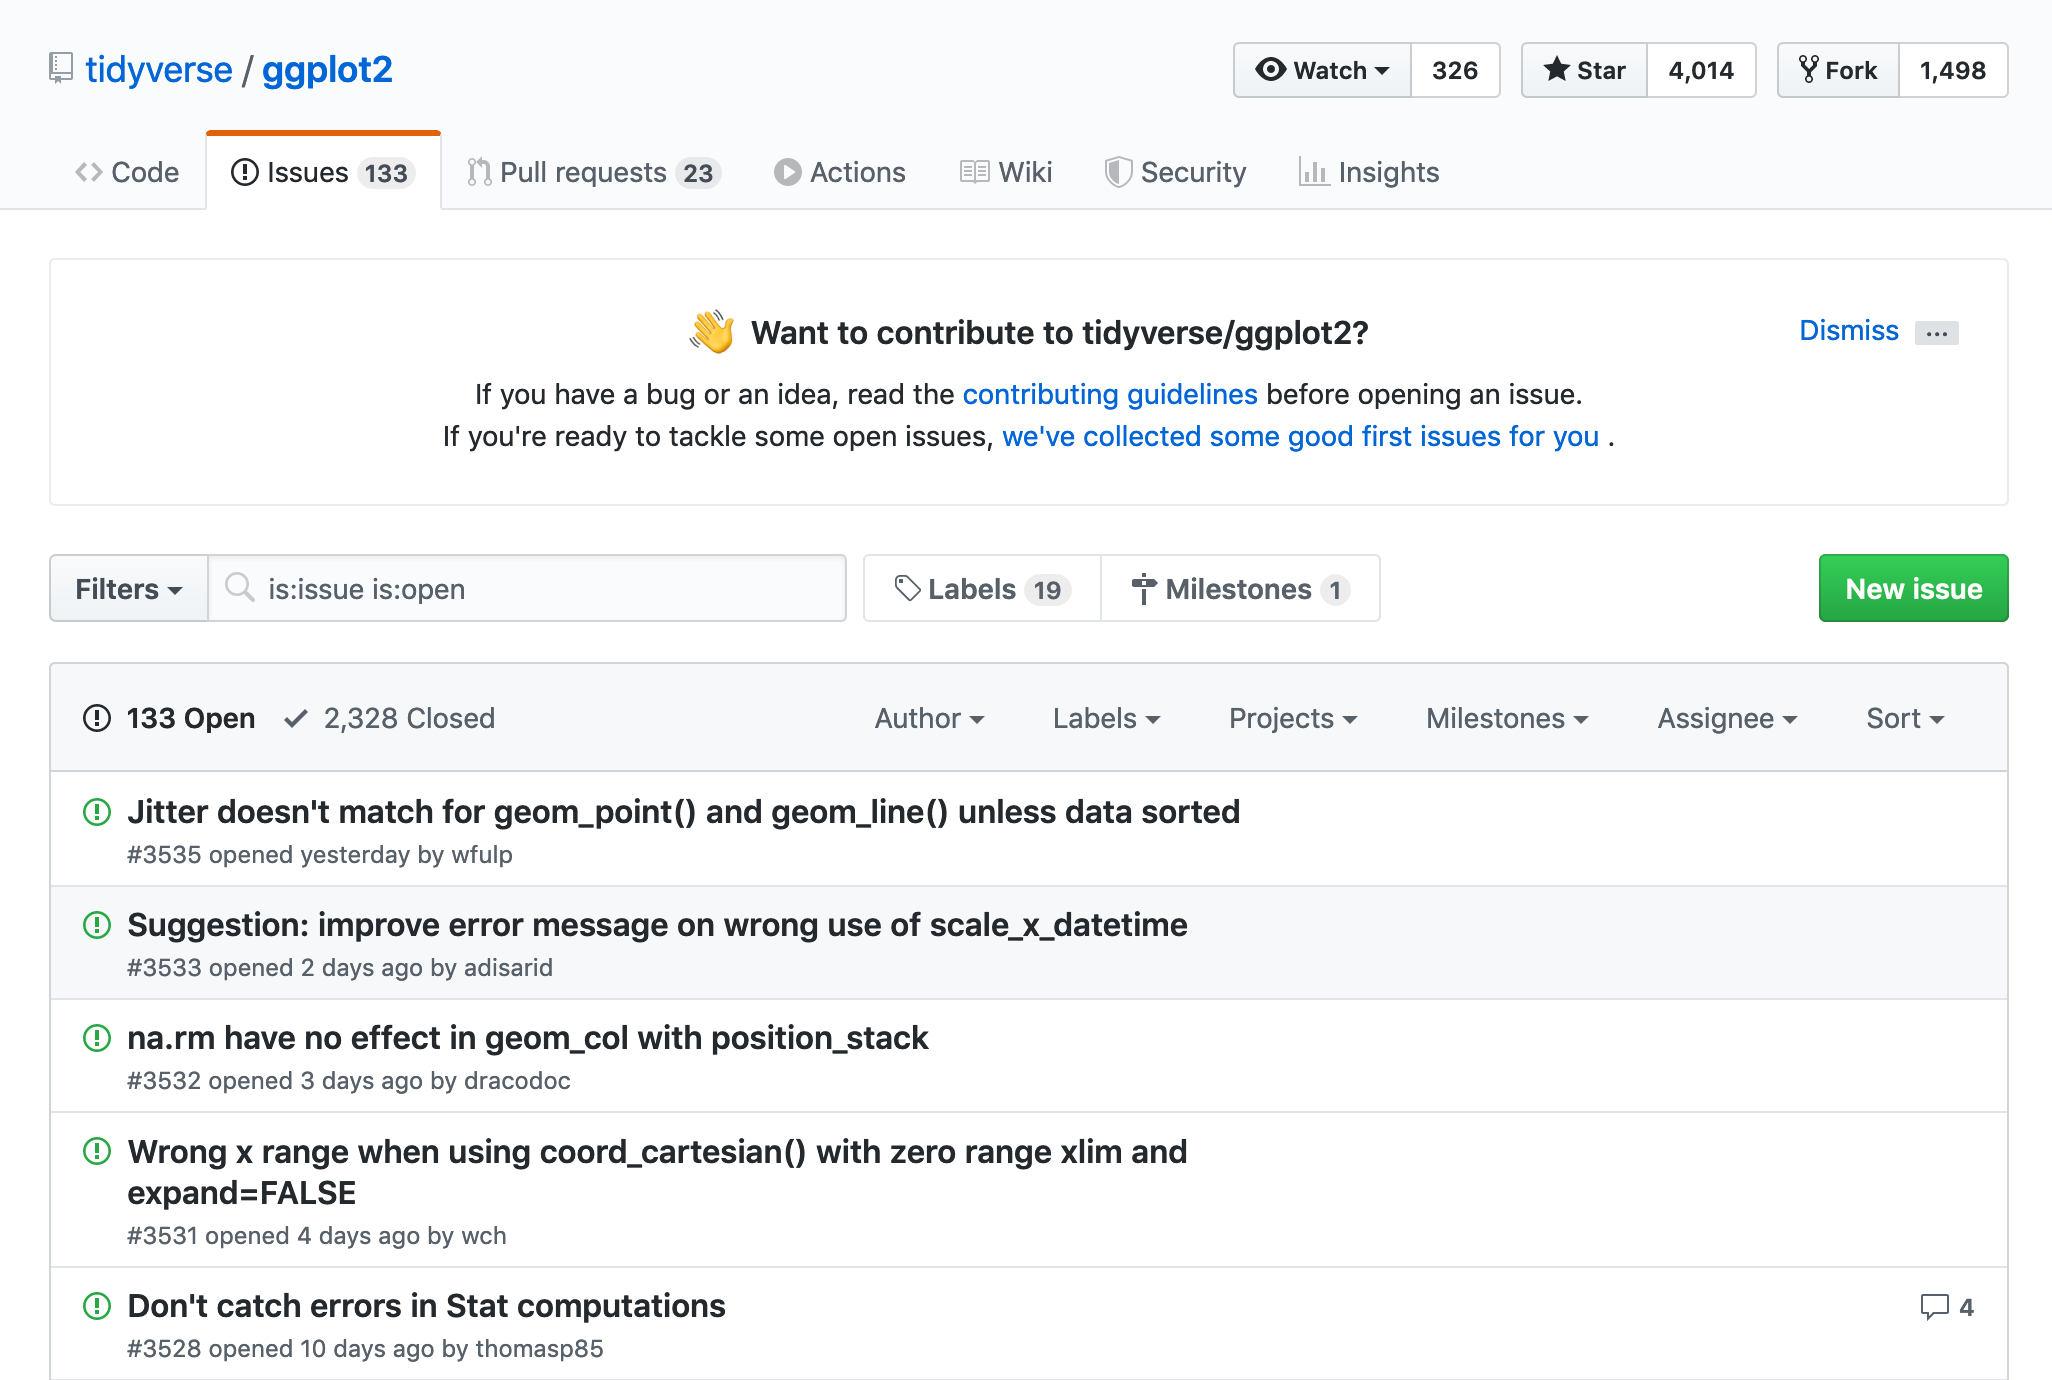
\includegraphics[width=0.8\textwidth,height=\textheight]{./img/issues-ggplot2.png}

\href{https://github.com/MozillaFestival/mozfest-program-2018/issues}{MozillaFestival's
Issues} are an example of a less ``traditional'', but increasingly
common use of Issues: for project submissions, coordination, and
community engagement. It is also an example of the use of labels: those
colorful tags that help group and categorize the Issues. To the right of
``Filters'', you'll see a ``Labels'' button: clicking on this will give
you a list of all the labels and how many Issues are tagged with each
label.

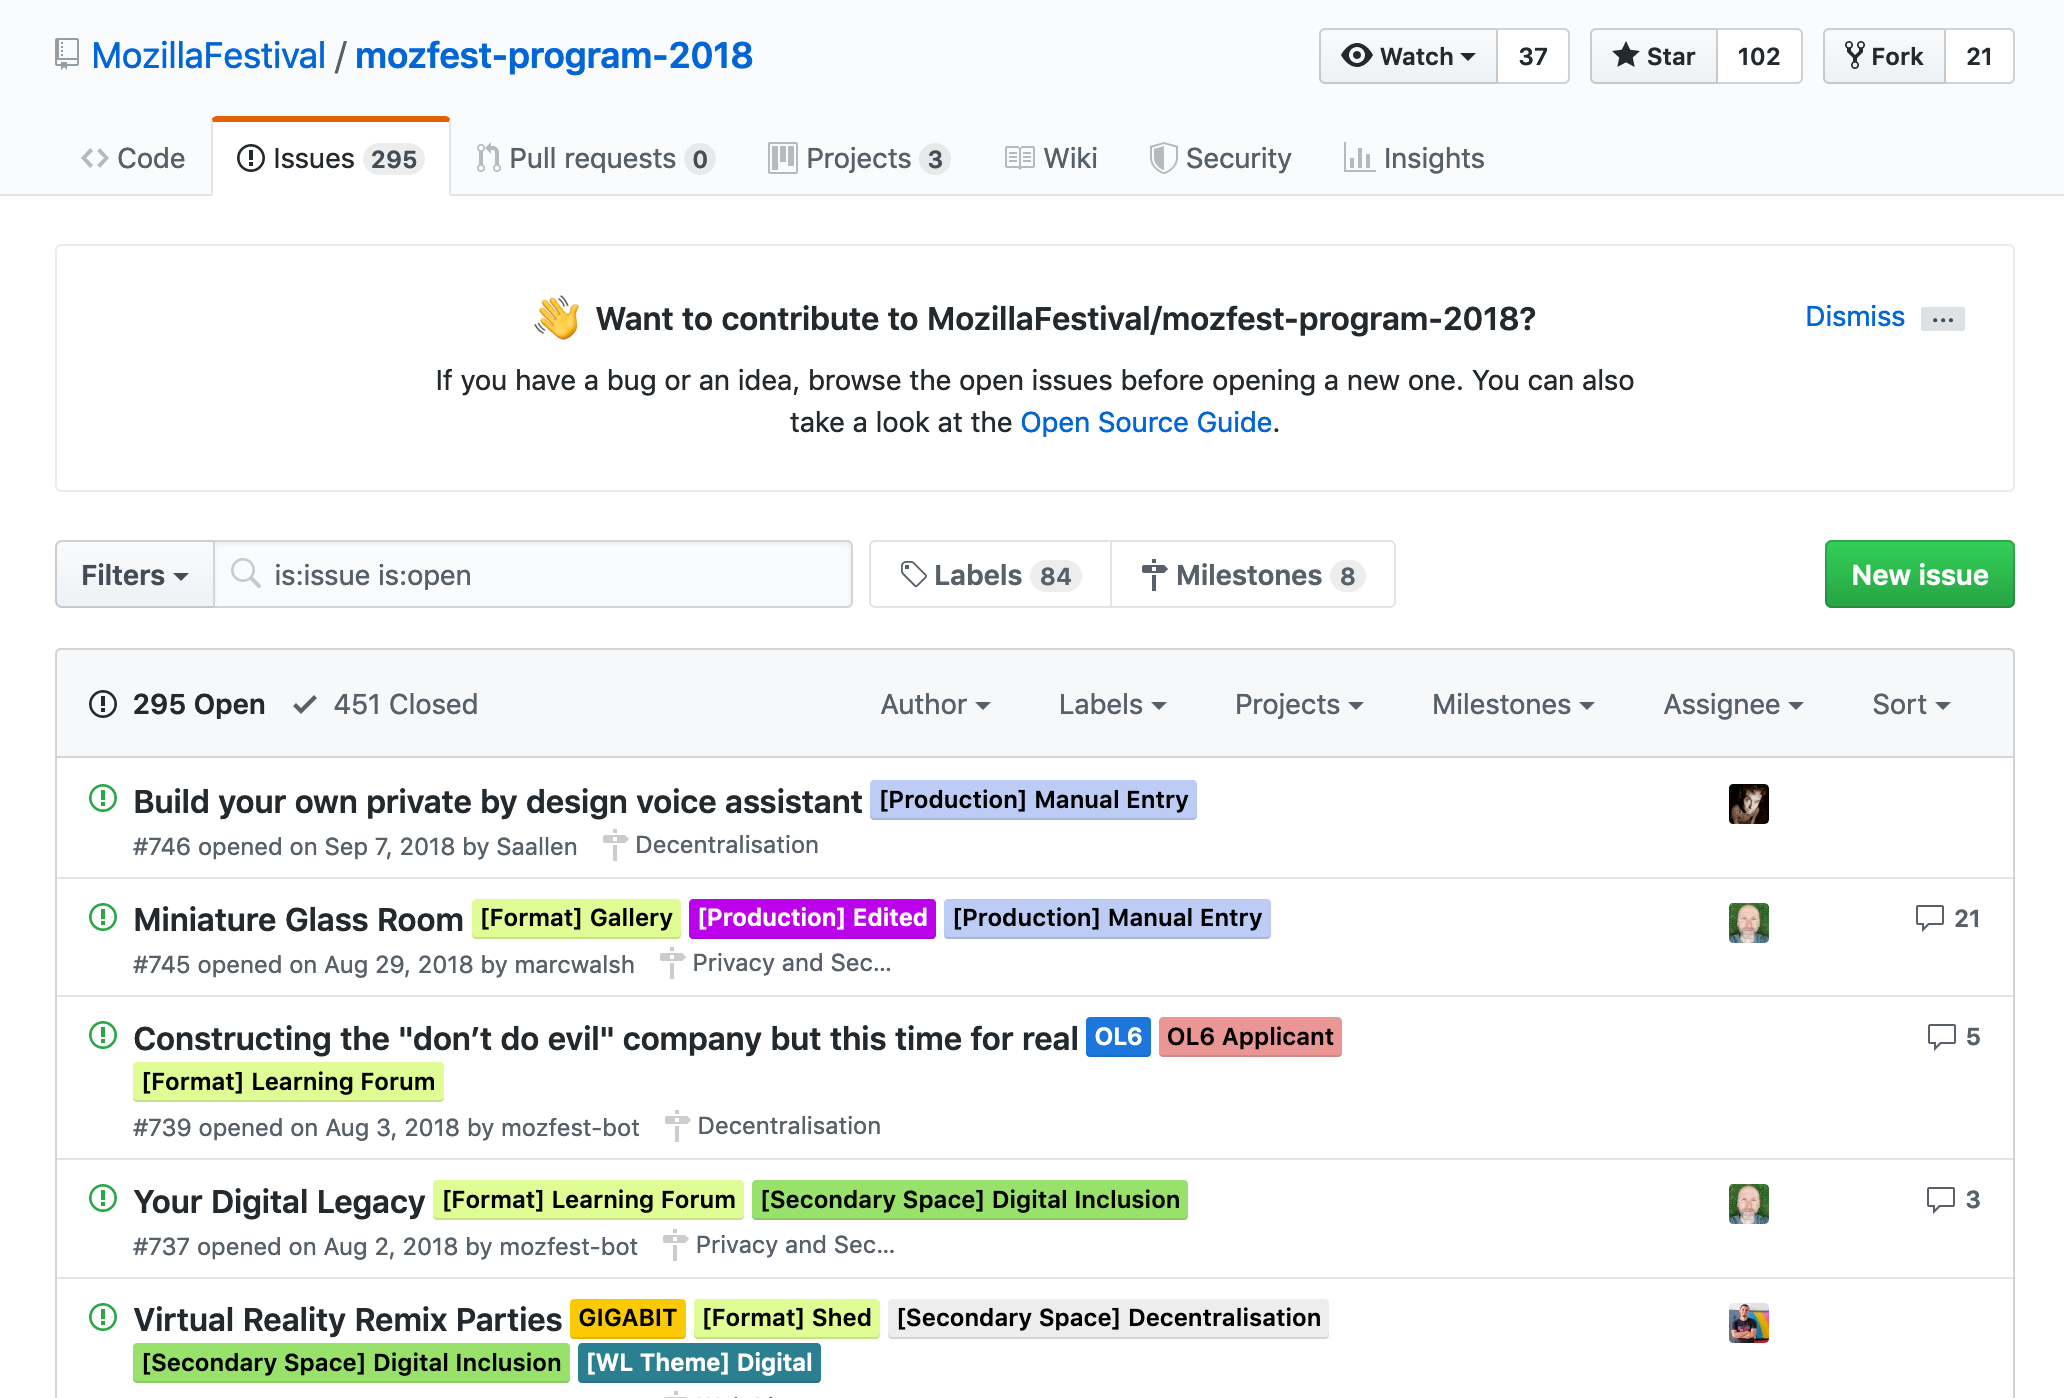
\includegraphics[width=0.8\textwidth,height=\textheight]{./img/issues-mozfest.png}

OHI-Science's Issues: are also an example of less ``traditional'' use of
Issues but perhaps also somewhat common. This is a private repository,
which is why there is no link to these Issues. Here, Issues are used for
private conversations and archiving ideas and discussions: the
OHI-Science team uses issues instead of email to have private, archived,
searchable conversations about scientific methods. We are diligent about
having important science conversations in these Issues, rather than
those conversations being lost in emails or Slack. This is more
organized and also makes onboarding team members much smoother since we
do not need to forward emails to new team members.

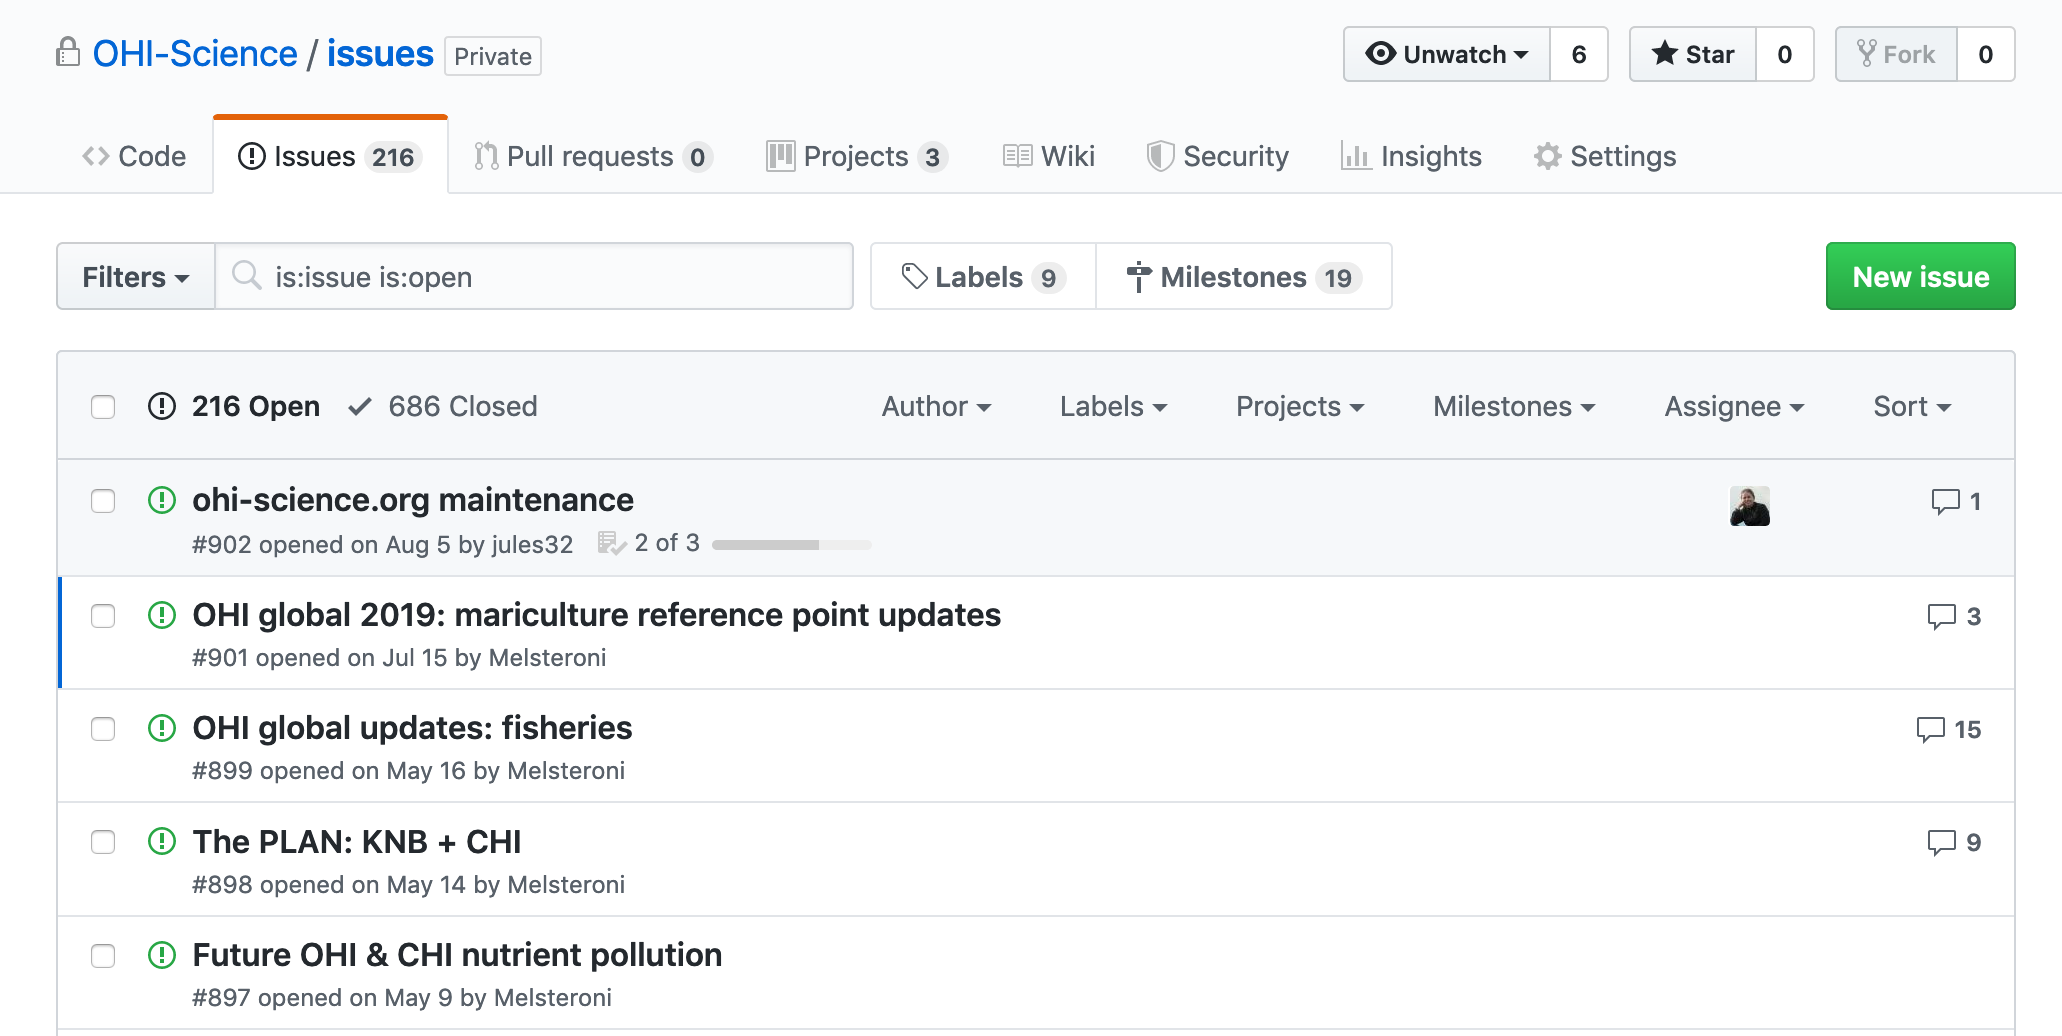
\includegraphics[width=0.8\textwidth,height=\textheight]{./img/issues-ohiscience.png}

\hypertarget{how-to-use-issues}{%
\section{How to use Issues}\label{how-to-use-issues}}

Let's do a demo with Issues.

\hypertarget{creating-a-new-issue}{%
\subsection{Creating a new Issue}\label{creating-a-new-issue}}

When you click on the green ``New Issue'' button'', you're asked to give
a Title and Leave a Comment. You can also attach files or images by
dragging them into the Issue.

Then you'll be able to Submit the Issue. On the right side, you'll see
options to Assign someone to the Issue, add a Label, add it to a
Project, or add it to a Milestone. We'll explore these features a bit
more in a moment.

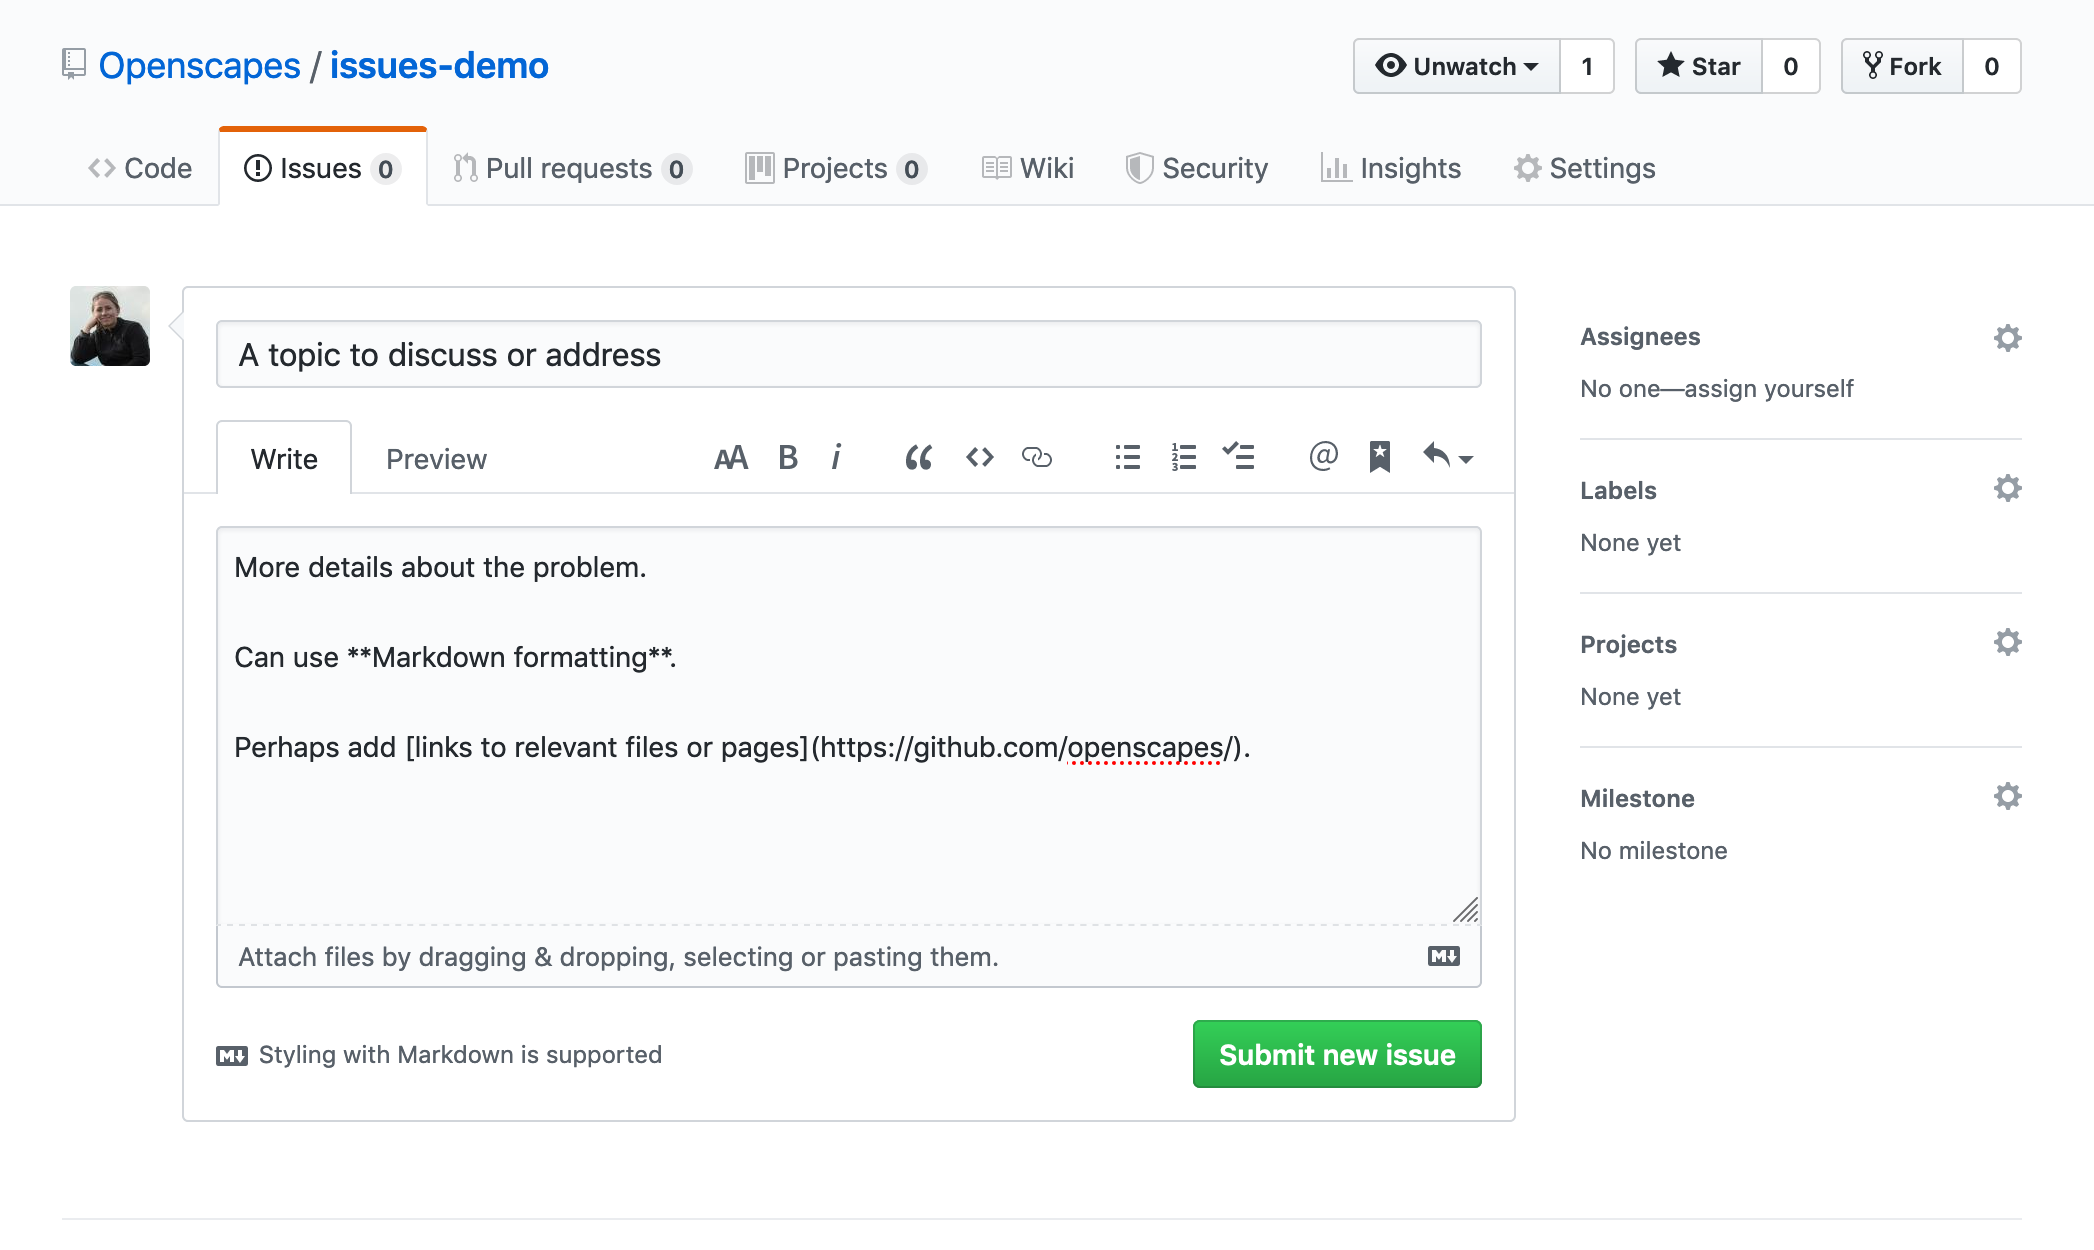
\includegraphics[width=0.8\textwidth,height=\textheight]{./img/issues-create.png}

When you click Submit, your Issue gets a number, which is now written
next to the title. This number is also part of the URL as well.

On the right of the Title, note that there is an ``Edit'' button if you
ever need to change the title of the Issue as the conversation evolves.
The Issue number will stay the same.

What happens if you want to edit the text of your Comment after you've
Submitted it? No problem. See that once you've submitted an Issue, there
is a blue bar at the top of the Comment, attributing your username to
this comment along with the date. At the very right of this blue bar,
there are 3 dots. Clicking here will give you the option to edit.

\hypertarget{commenting}{%
\subsection{Commenting}\label{commenting}}

The great thing about Issues is that they are for conversations with
yourself and others. So once you've submitted an Issue, you can string
together additional Comments within this comment. Maybe you asked a
question, and someone else will respond with a solution or idea. They
might link to an Issue with a related topic, or an external link that
might be helpful.

You can also tag people in Issue Comments with the ``@'' symbol. As
noted above, anyone who is part of the repository will automatically get
email notifications when comments are submitted. But tagging specific
users will also send them an email, and is a good way to bring folks
into the conversation who might not already be ``watching'' the whole
repository. In a public repository you can tag any GitHub user, and in a
private repository they have to have permission.

Each time there is a comment in the Issue thread, there will be a new
date marked in the blue bar at the top of the Issue. This is a nice way
to see how current conversations are.

And something really great is that you can click on the date --- and
watch the URL change. This allows you to anchor to a specific comment
within the Issue thread. This is really useful if, for example, you
wanted to share a specific comment with someone else instead of having
them scroll down themselves. (Note: you can also click on the three dots
at the right of the blue Comment header to copy the anchored link).

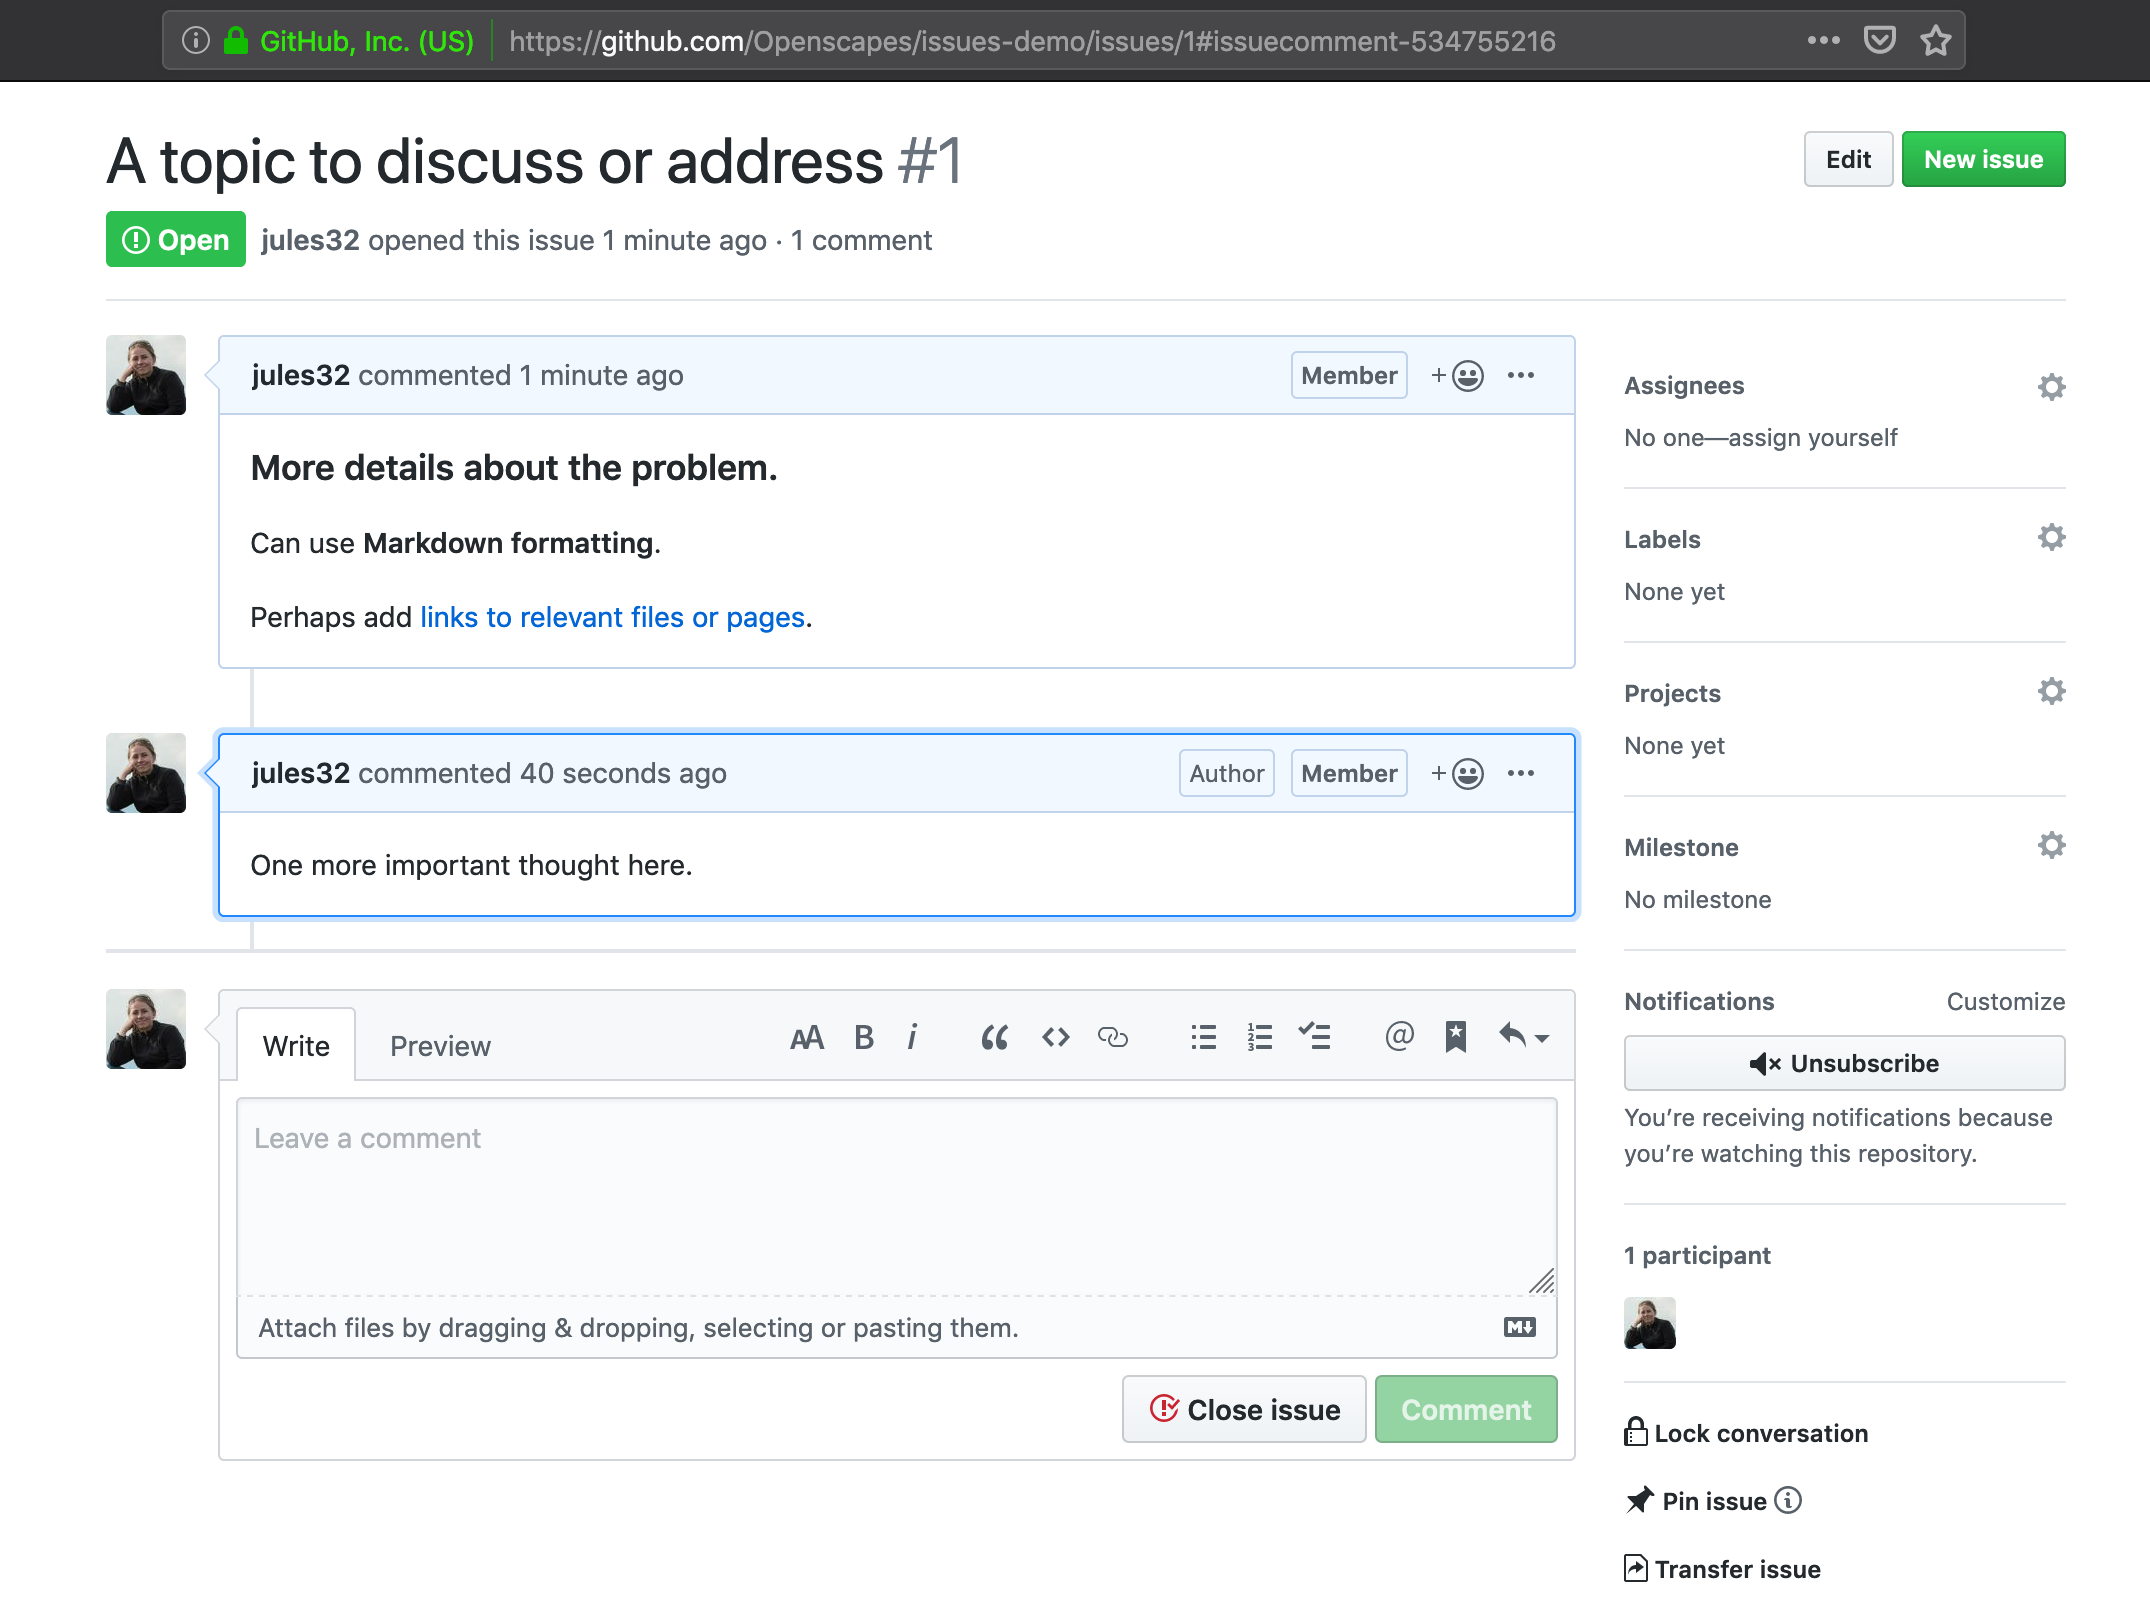
\includegraphics[width=0.8\textwidth,height=\textheight]{./img/issues-comment.png}

\hypertarget{markdown}{%
\subsection{Markdown}\label{markdown}}

Issues support Markdown. This means that you can add simple formatting
to your text, such as headers, bold and italics, lists, images, links,
and formatted code. To help you use Markdown formatting as you learn,
GitHub Issues have built-in help: there are icons between the Title and
the Comment of the Issue that will do the Markdown formatting for you,
and help you learn along the way.

There is also a ``Preview'' tab between the Title and Comment (next to
the ``Write'' tab, where you are by default) where you can preview what
your Markdown formatting looks like before you Submit the Issue.
Submitting the Issue will also render the Markdown formatting.

GitHub enables you to also create Markdown check-lists by typing
\texttt{-\ {[}\ {]}}. Once this is rendered, you can click it to check
this box. Alternatively, in Markdown you check a box by typing
\texttt{-\ {[}x{]}}. The number of checked and unchecked items will be
visible in the Issue as well.

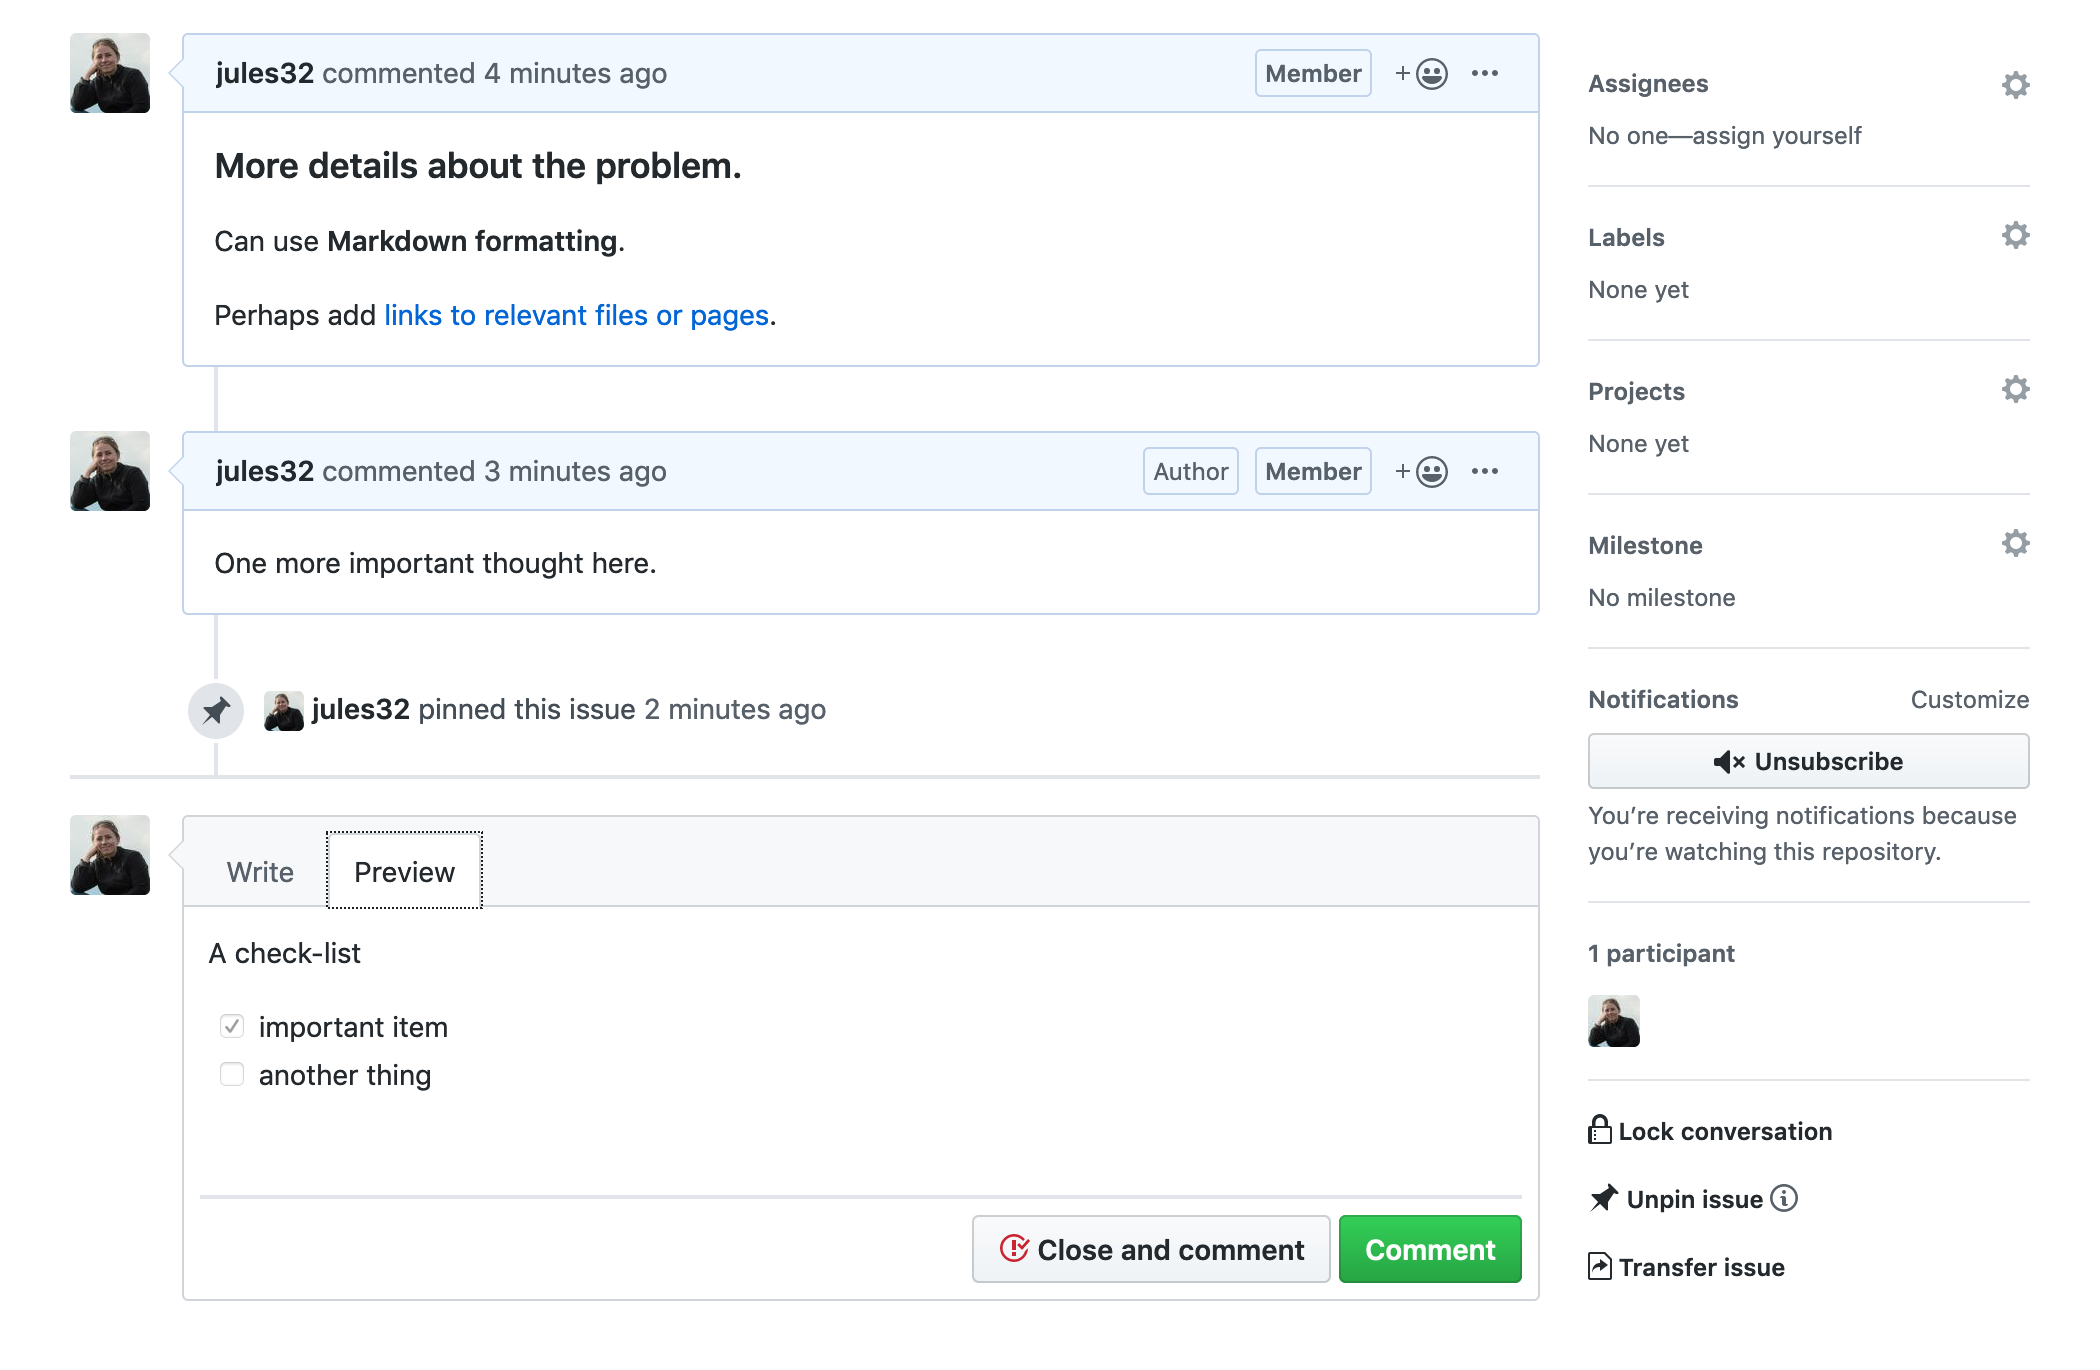
\includegraphics[width=0.8\textwidth,height=\textheight]{./img/issues-checklist.png}

\hypertarget{linking-to-files}{%
\subsection{Linking to files}\label{linking-to-files}}

Linking to specific files or versions of files is good practice when you
are discussing it in an Issue: reduce the work for the person reading
the Issue (which might be Future You!). You can link to the file by
opening it in the browser and copying its URL and placing it in Markdown
formatting for hyperlinks: \texttt{{[}text\ to\ hyperlink{]}(URL)}.

You can also navigate to a specific version of that file, or a specific
commit message, if you want to capture that file at a specific point in
time.

You can also anchor to specific lines within a file, which is useful if
you are requesting feedback on a specific part of an analysis or asking
for help troubleshooting. I can send someone to a specific place within
a file with the appropriate lines highlighted. For example
\texttt{{[}important\ code{]}(https://github.com/Openscapes/issues-demo/blob/master/code-example.R\#L12-L13)}
will render as
\href{https://github.com/Openscapes/issues-demo/blob/master/code-example.R\#L12-L13}{important
code}.

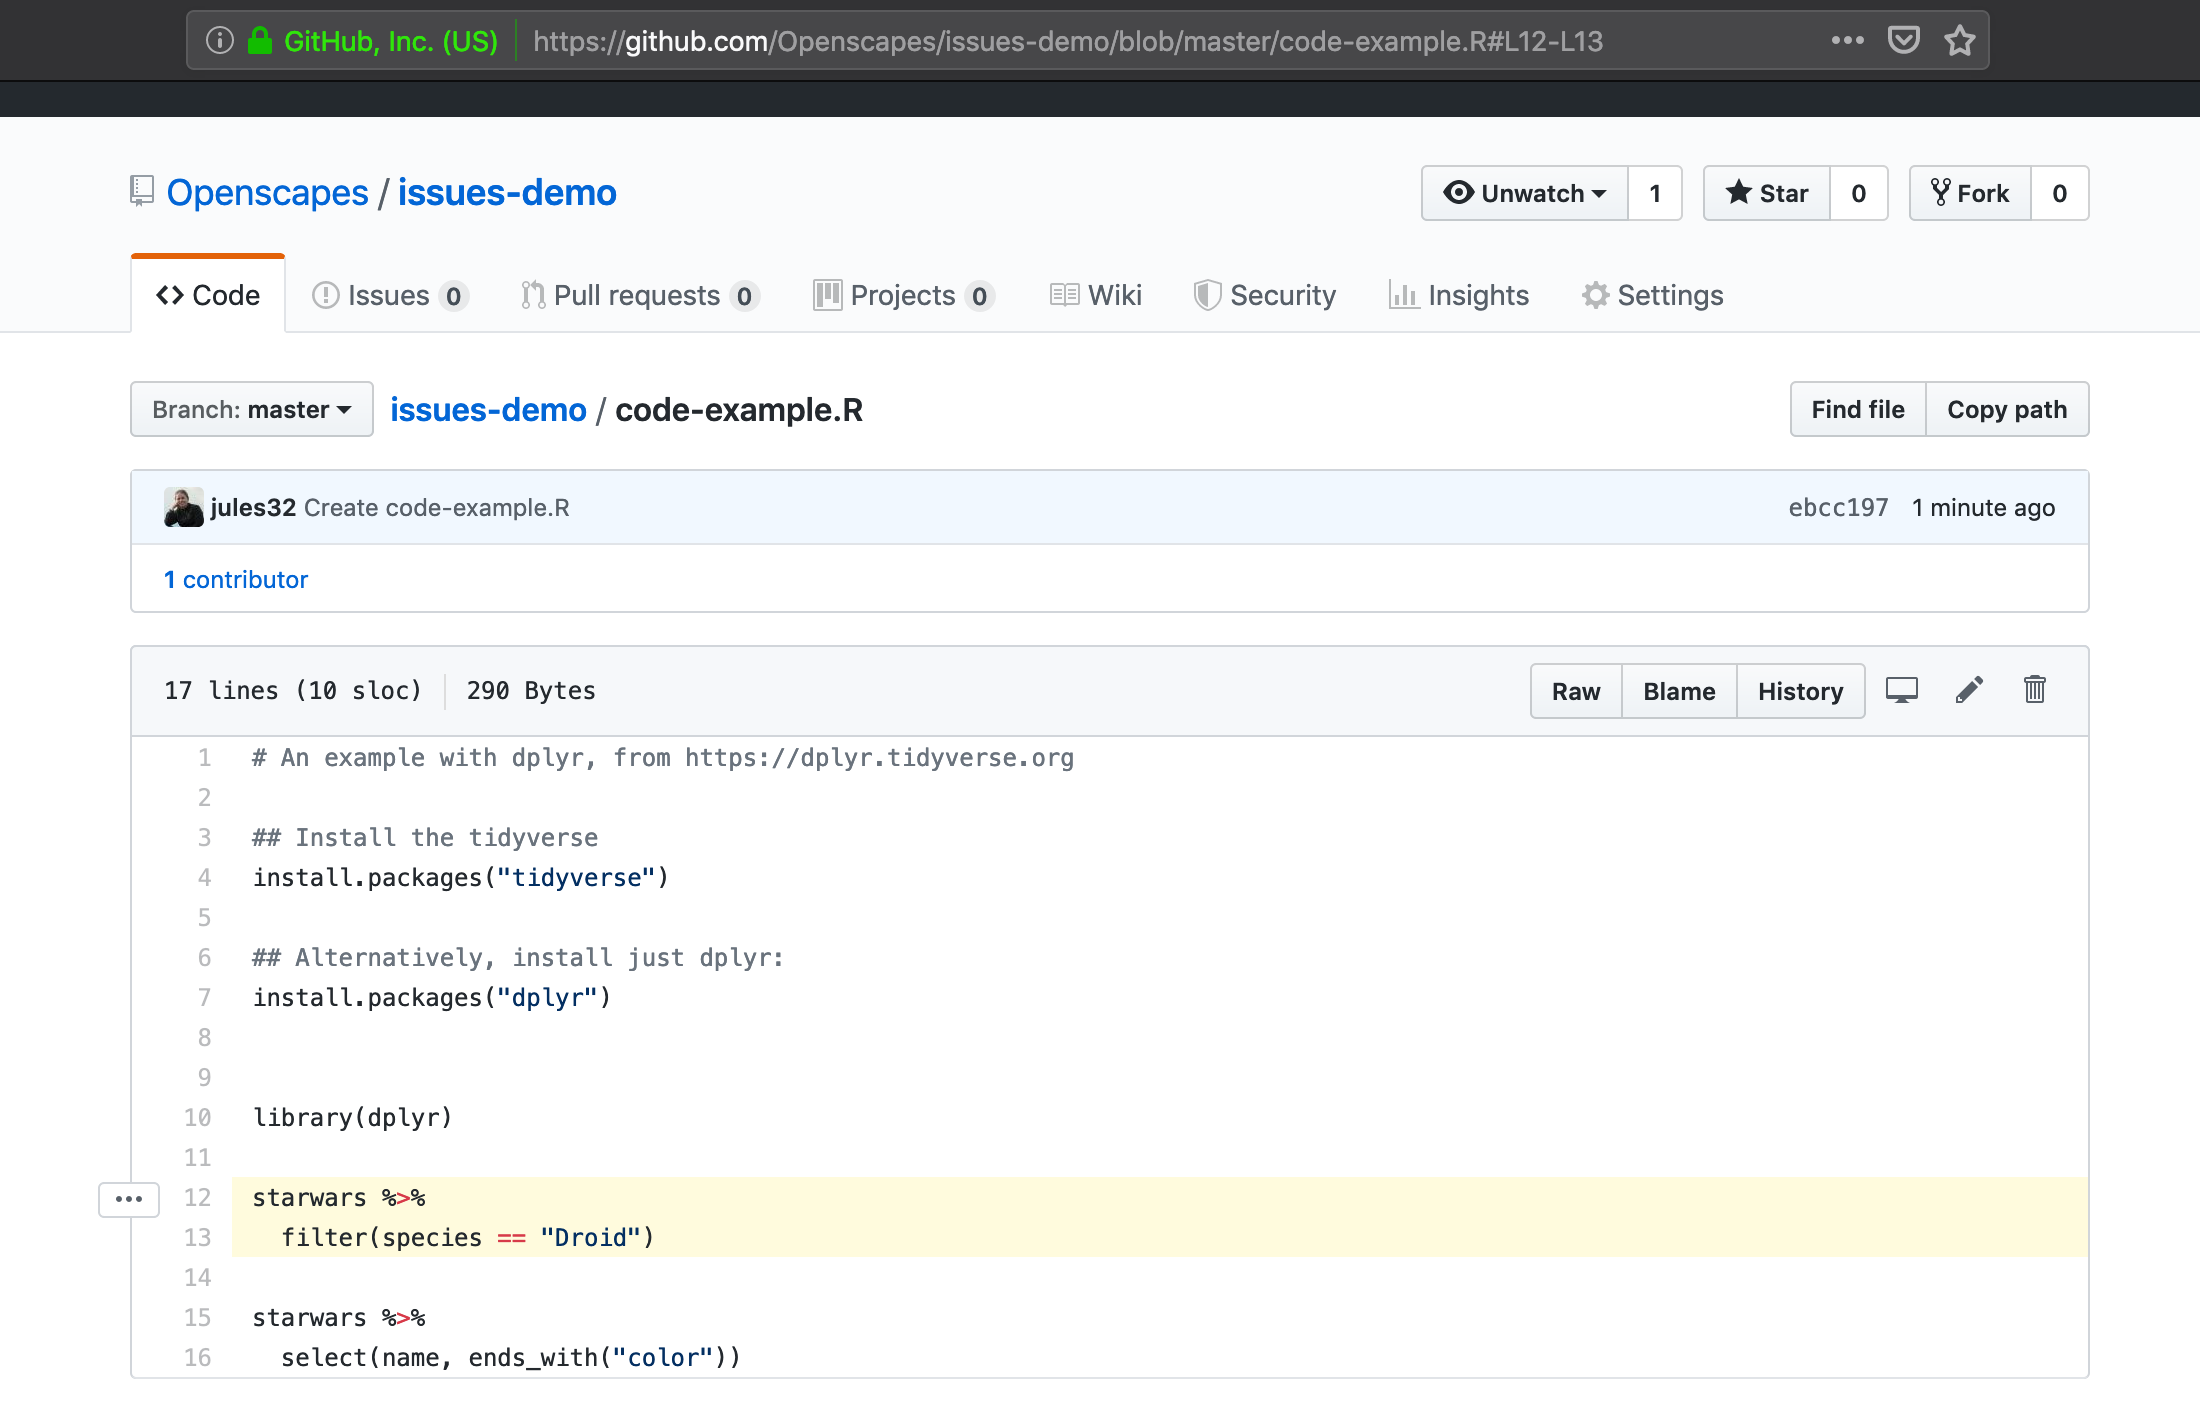
\includegraphics[width=0.8\textwidth,height=\textheight]{./img/github-anchor-lines.png}

\hypertarget{assigning-labels}{%
\subsection{Assigning, Labels}\label{assigning-labels}}

On the right side of the Issue thread, there is the ``metadata'' for the
Issue. You can assign the Issue to a specific user, or label it with a
suite of labels that you can customize (when you click on labels, see
all the way at the bottom the option to edit labels. And there are other
ways to navigate there as well).

If you navigate back to the full list of Issue topics (which will have
the URL github.com/username-or-organization/repo-name/issues), you'll
see these metadata categories listed at the top as well, which lets you
filter or view based on these categories.

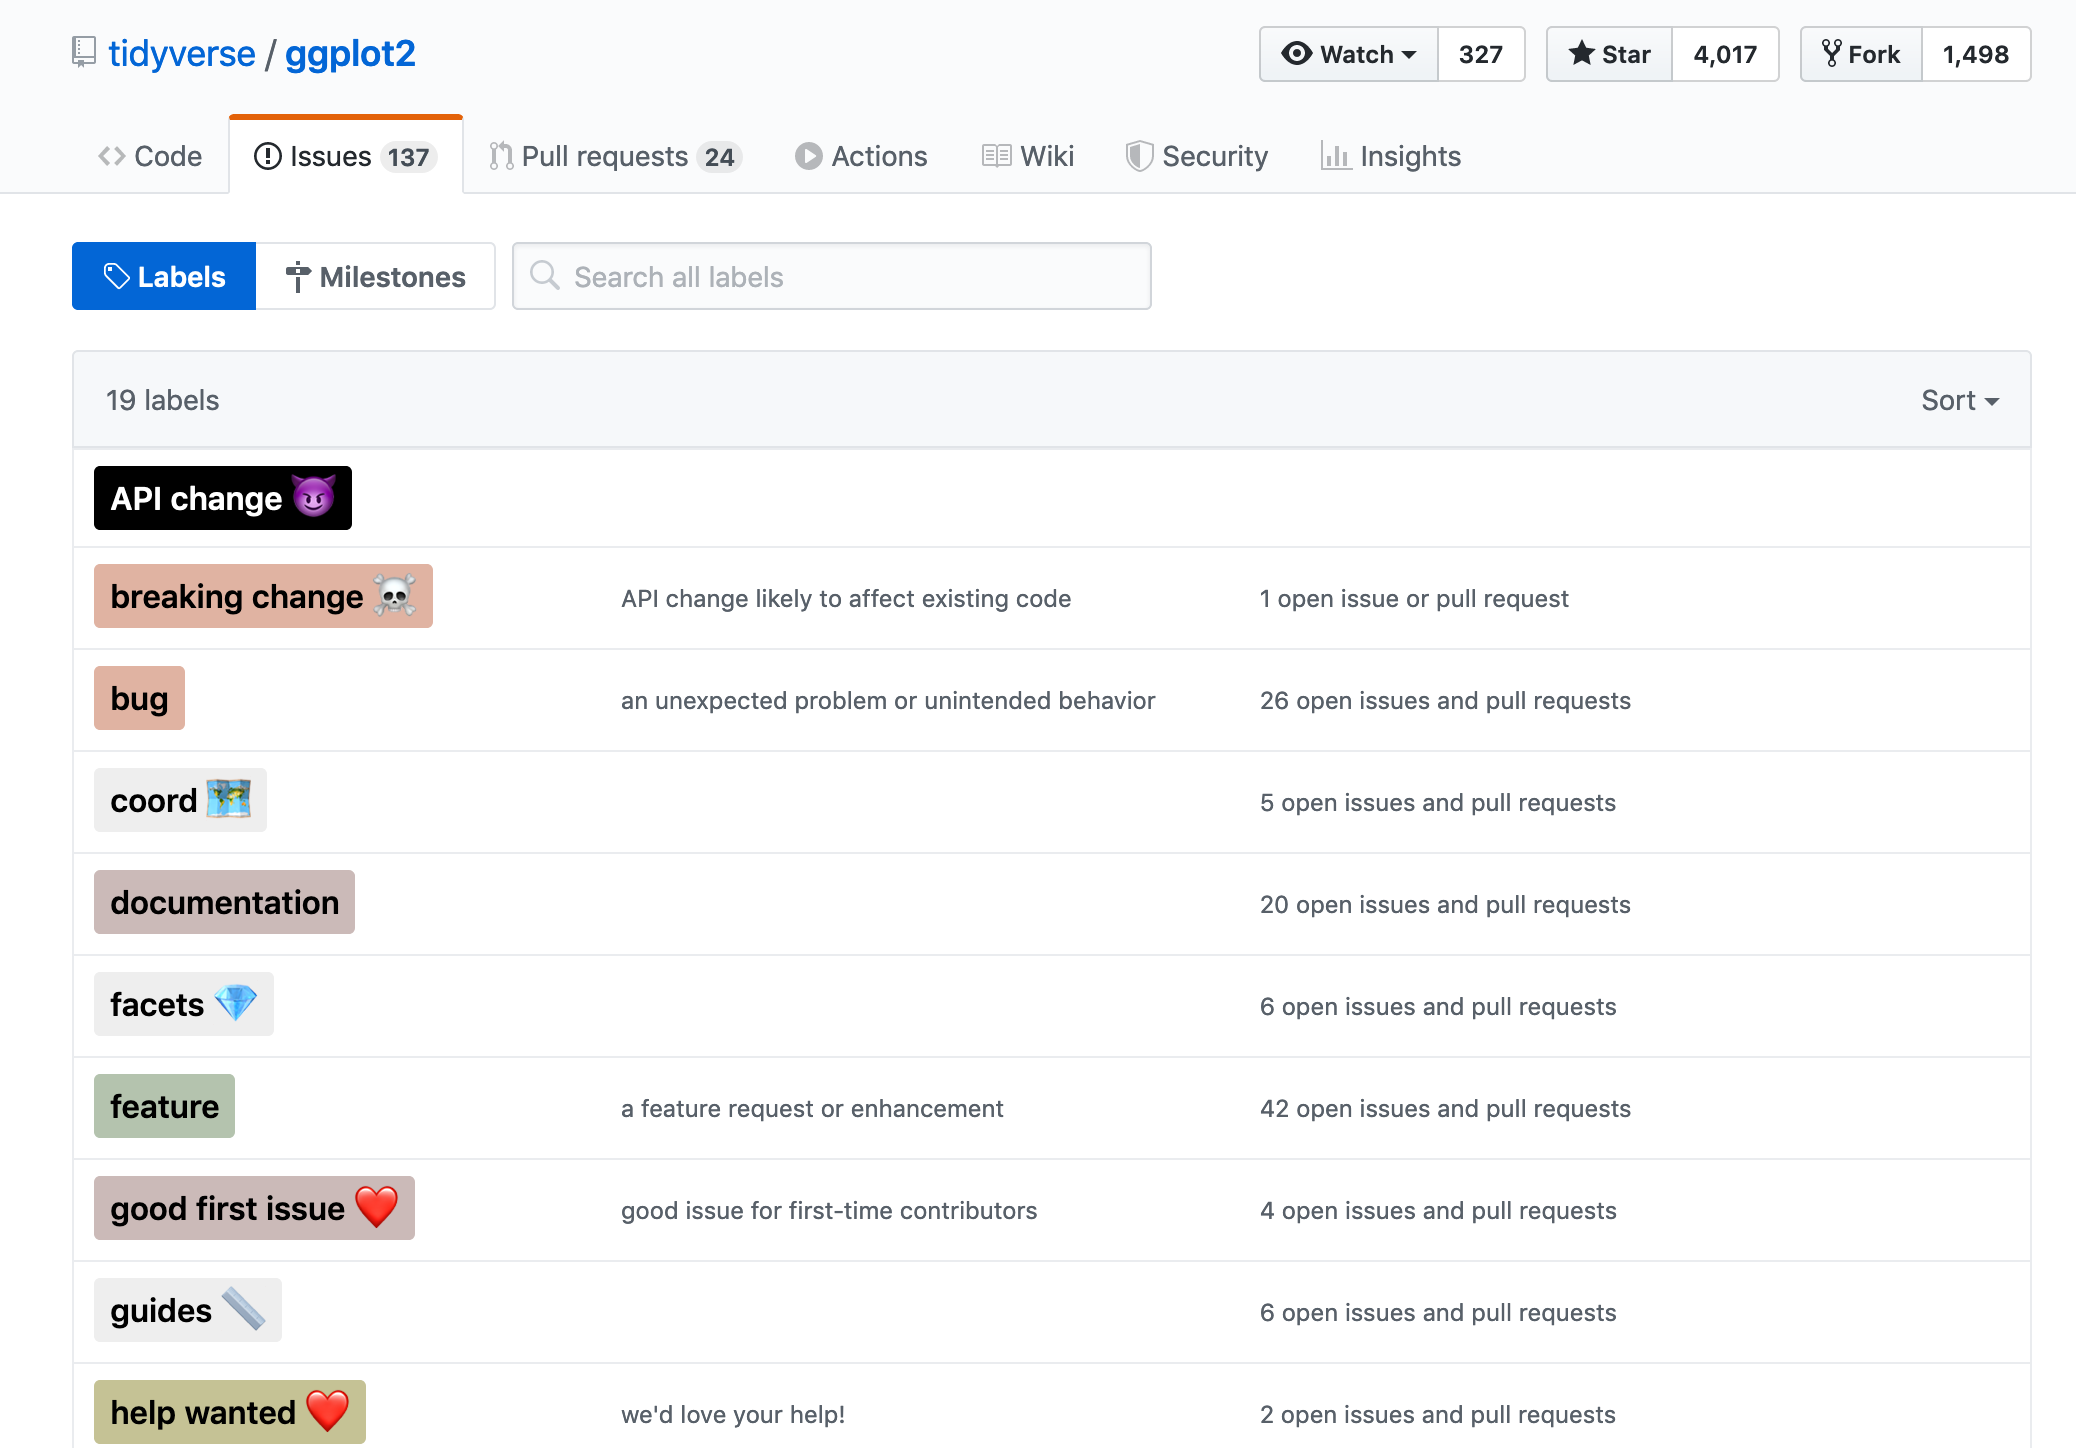
\includegraphics[width=0.8\textwidth,height=\textheight]{./img/issues-labels.png}

\hypertarget{projects-milestones}{%
\subsection{Projects, Milestones}\label{projects-milestones}}

Projects and Milestones are further ways to organize and track progress
with your Issues.

Projects are a way to organize and prioritize your issues. It uses the
idea of a Kanban board, which
\href{https://en.wikipedia.org/wiki/Kanban_board}{Wikipedia} says
``visually depict work at various stages of a process using cards to
represent work items and columns to represent each stage of the process.
Cards are moved from left to right to show progress and to help
coordinate teams performing the work.'' The simplest have 3 columns
labeled ``to do'', ``doing'' and ``done''.

You can use Projects for both Organization or personal projects. In
fact, you can have multiple projects within the same repository, so
different people can have different Projects organized within their
shared repository, for example.

You have a lot of control over how you will manage your Projects; at
this point I do not use all the features but have been playing around
with using them for Openscapes planning:

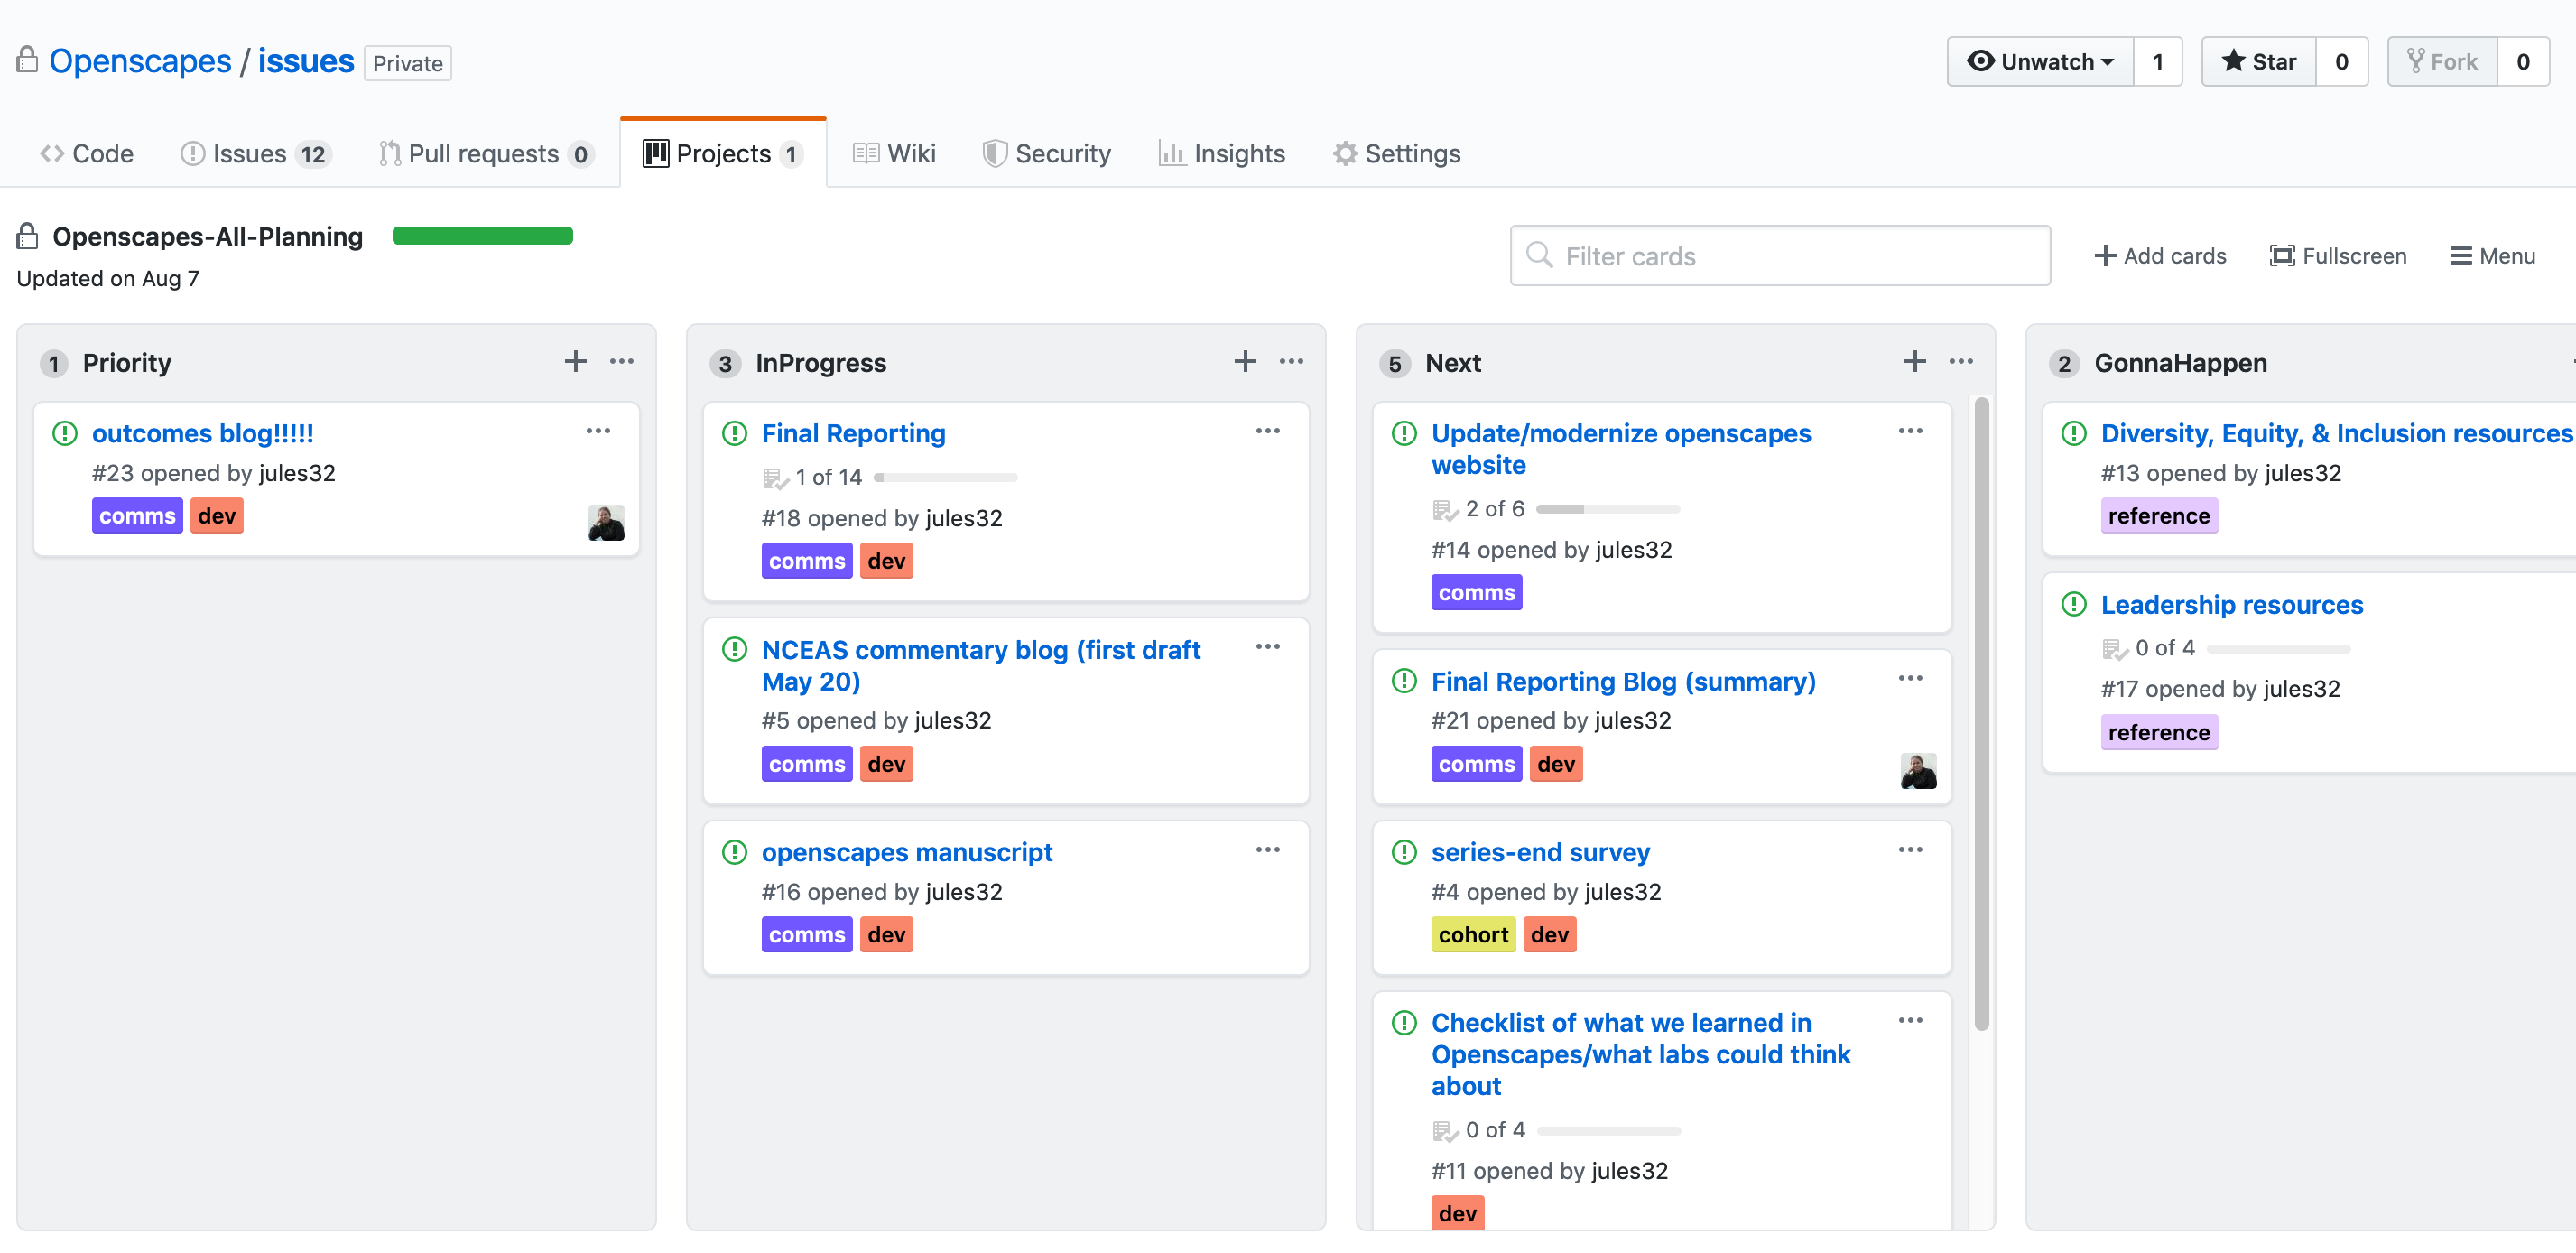
\includegraphics[width=0.8\textwidth,height=\textheight]{./img/issues-projects.png}

Milestones are a way to attach deadlines to your Project (although you
do not need to identify a date if you don't want to). Once you create a
Milestone, you can add Issues to that Milestone to help track progress.
For example, maybe you have a presentation coming up and there are
several Issues that need to be addressed before then.

\hypertarget{strategies-for-issues}{%
\section{Strategies for Issues}\label{strategies-for-issues}}

Every repo has Issues, but do you want to use Issues in every repo? It
helps to consider the purpose for the Issues.

Using Issues for ``traditional'' bug/features for code, it makes sense
to keep the repository public and have all Issues pertaining to that
repo there within that repo.

If you're using Issues for ``non-traditional'' laboratory research group
and science conversations, there are other considerations. Maybe you do
want a private repository, but even so you'll want to think ahead. Will
you eventually make that repo public when you publish your study?
Changing a repo from private to public (or vice versa, both are possible
in the repository's Settings) will make not only the code and files of
that repo public, but also all the Issues. Which is fine, but it might
add considerations in terms of what is discussed in those Issues.

\hypertarget{ohi-example}{%
\subsection{OHI example}\label{ohi-example}}

Here is an example of the Ocean Health Index team's thought process \&
strategy.

Our team works within a GitHub Organization called ``OHI-Science''.
Within that Organization, we work in many repositories, with different
combinations of people working primarily within different repositories.
Sanity-wise, we didn't want to have conversations in Issues within each
of those repositories because it would make finding those conversations
more difficult (although now GitHub can search all Issues/code across an
Organization!).

We also wanted our repos to be public, but to have private conversations
using the Issues feature.

These two needs led us to create a single private repository named
``issues'', and we only use it for Issues. This works really well for
us, especially since our team lead can engage in these discussions by
receiving emails about the Issues in his inbox, and can respond without
having to go to GitHub.com.

\hypertarget{your-turn-create-comment-on-issues}{%
\section{Your Turn: Create \& comment on
issues}\label{your-turn-create-comment-on-issues}}

We will break into groups and you can explore some of these features in
Issues. Here is what to do:

\begin{itemize}
\tightlist
\item
  Go to
  \href{https://github.com/openscapes/demo/issues}{github.com/openscapes/demo/issues}
\item
  Create an issue, tag people in your breakout group (ask for their
  username)
\item
  Browse issues, comment in other issues
\item
  Try:

  \begin{itemize}
  \tightlist
  \item
    Linking to the .md document you created in the previous chapter
  \item
    Creating a label and applying it, assigning people
  \item
    Adding Issues to a Project (create one if need be)
  \item
    Closing an Issue
  \end{itemize}
\end{itemize}

Have fun! And throughout the process, talk to your breakout group, and
share what you learn.

Here's what your inbox will look like afterwards:

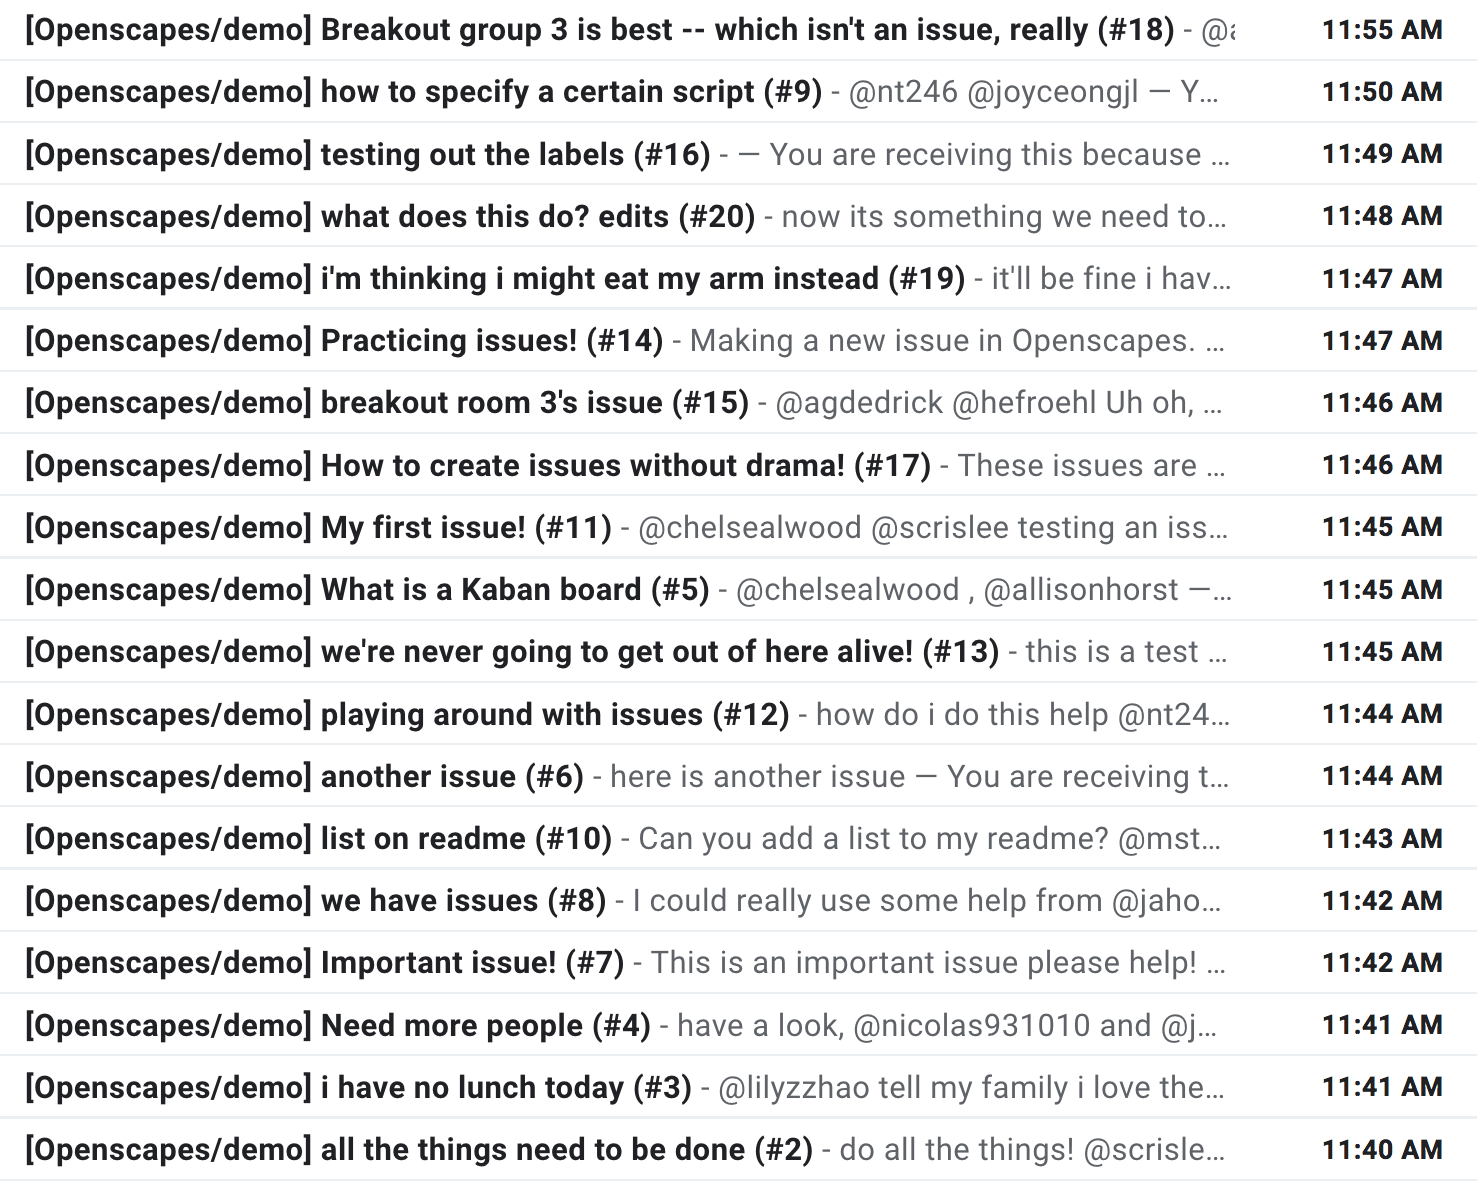
\includegraphics[width=0.8\textwidth,height=\textheight]{./img/issues-inbox-crop.png}

This is pretty rare to receive so many emails all at once. But you can
always switch your setting to ``Not Watch'' this repository so that you
only receive emails about Issues that you are tagged in.

\hypertarget{r-scicomm}{%
\chapter{RMarkdown for scicomm}\label{r-scicomm}}

\emph{Coming soon.
\href{https://docs.google.com/presentation/d/1efJj7Dxg_g4ZRZT2b1agDQrT3DN5lVcNvv25IWcyGlw/edit?usp=sharing}{Slides}
are best until then}. See also
\href{https://docs.google.com/presentation/d/1Jv0akRHEnjG_4t_9P7t93682BCBJskYnRu_7EnaeDQI/edit?usp=sharing}{Data
science as an entryway to open publishing} - May 27, 2020: Fireside Chat
co-presented with Dr.~Nick Tierney at
\href{https://openpublishingfest.org/calendar.html\#event-74}{Open
Publishing Fest}

So much potential for public communication, lab protocols and documents,
etc. with R.

All based on RMarkdown.

\hypertarget{books-with-bookdown}{%
\section{books with bookdown}\label{books-with-bookdown}}

Commit the generated docs/ directory!

Then, change the setting in your repo on github.com so that github knows
where your book is located so it can publish it. Here's what to do:

\begin{enumerate}
\def\labelenumi{\arabic{enumi}.}
\tightlist
\item
  go to https://github.com/haudarren/ai\_handbook
\item
  click on settings at the top bar (at the opposite end from code,
  issues, pull requests)
\item
  scroll down to the GitHub pages section. Click on Source and change it
  so it reads master branch /docs folder like below. You should get a
  green band like below that says ``your site is published to
  username.github.io/reponame''
\end{enumerate}

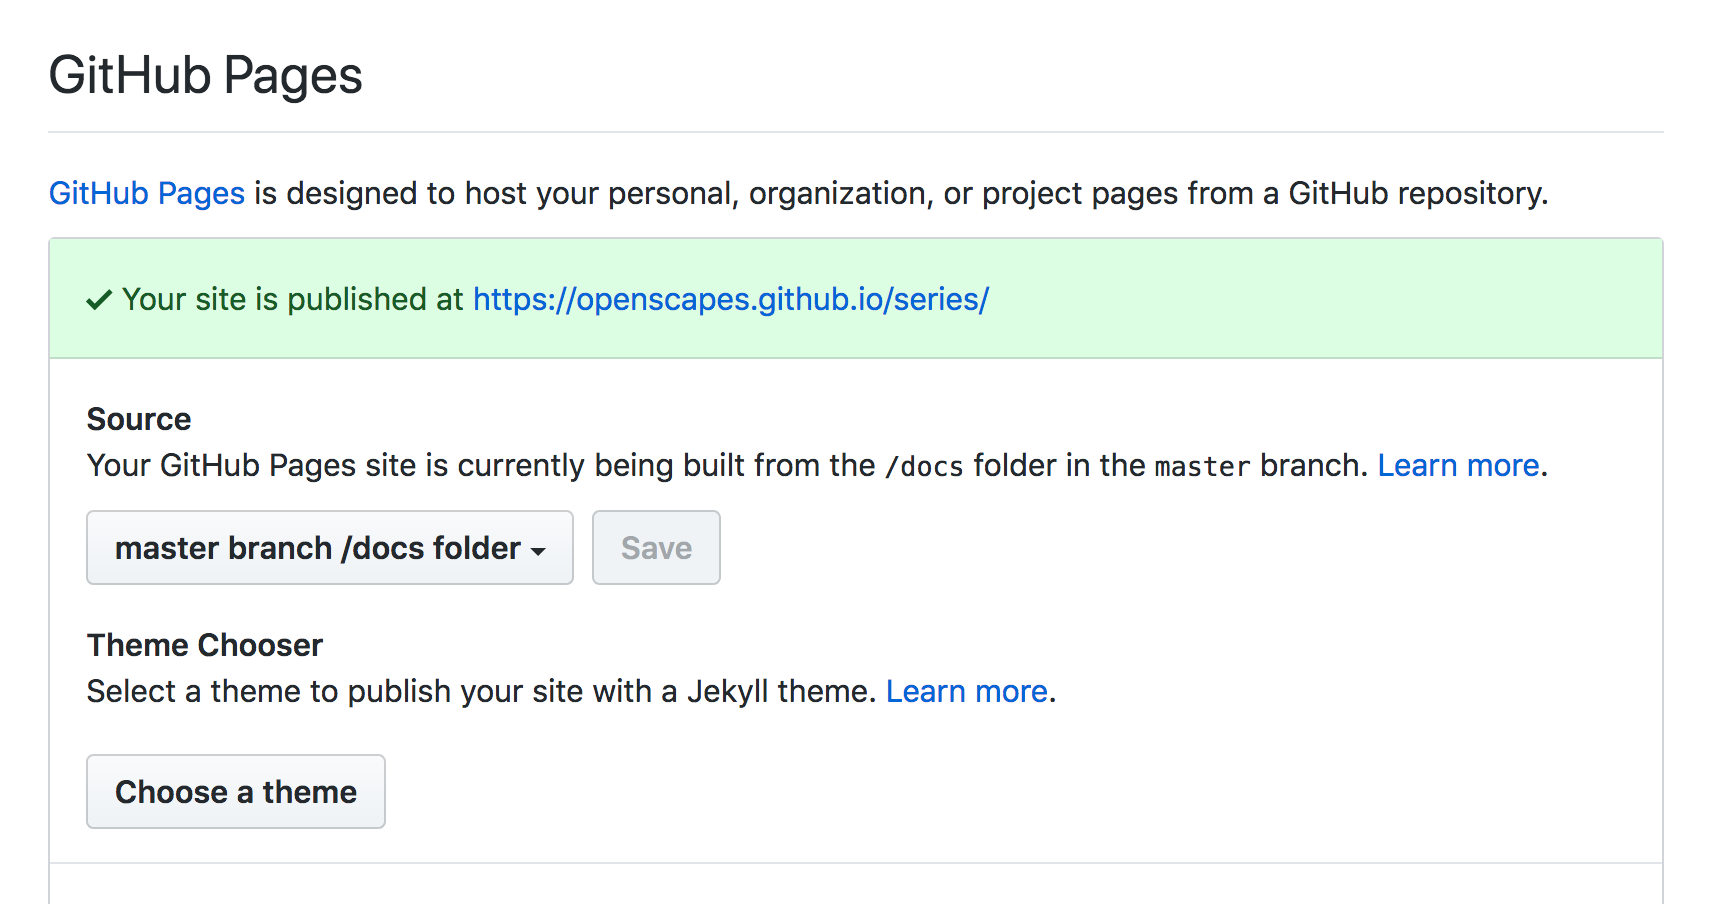
\includegraphics{./img/github-bookdown-docs-setting.png}

\hypertarget{websites-with-rmarkdown}{%
\section{websites with RMarkdown}\label{websites-with-rmarkdown}}

simple, static

\hypertarget{websites-with-blogdown}{%
\section{websites with Blogdown}\label{websites-with-blogdown}}

fancier, dynamic

\hypertarget{further-resources-3}{%
\section{Further resources}\label{further-resources-3}}

\begin{itemize}
\tightlist
\item
  \href{https://rmarkdown.rstudio.com}{RMarkdown} - RStudio (2021)
\item
  \href{https://alison.rbind.io/post/2020-05-28-how-i-teach-r-markdown}{How
  I teach RMarkdown} - Hill (2020)
\item
  \href{https://rmd4sci.njtierney.com}{R Markdown for scientists} -
  Tierney (2020)
\item
  \href{https://rstudio-conf-2020.github.io/r-for-excel}{R for Excel
  Users} - Lowndes \& Horst (2020)
\item
  \href{http://jules32.github.io/rmarkdown-website-tutorial}{RMarkdown
  website tutorial} - Lowndes (2016)
\item
  \href{https://danovando.github.io/publications-with-rmarkdown/presentations/pubs-with-rmarkdown\#9}{Academic
  Publications with R Markdown}- Ovando 2020
\end{itemize}

\hypertarget{resources-influence}{%
\chapter{Resources that influence us}\label{resources-influence}}

\emph{Some resources that influence our thinking.}

\hypertarget{talking-about-data-science-hilary-parker-roger-peng}{%
\section{Talking about data science: Hilary Parker \& Roger
Peng}\label{talking-about-data-science-hilary-parker-roger-peng}}

\href{https://rstudio.com/resources/rstudioconf-2020/not-so-standard-deviations-episode-100/}{RStudio::conf(2020)
keynote} \&
\href{http://nssdeviations.com/100-live-from-rstudio-conf-2020}{NSSD
podcast episode 100}

\begin{quote}
If you want to write, you read a lot, music, you listen a lot. I'ts hard
to do this with data analysis.
\end{quote}

\hypertarget{opinionated-data-analysis}{%
\section{Opinionated data analysis}\label{opinionated-data-analysis}}

\hypertarget{principles-for-data-analysis-workflows}{%
\section{Principles for data analysis
workflows}\label{principles-for-data-analysis-workflows}}

Stoudt, Vásquez, Martinez,
https://journals.plos.org/ploscompbiol/article?id=10.1371/journal.pcbi.1008770

\begin{quote}
workflow describes what a researcher does to make advances on scientific
ques- tions: developing hypotheses, wrangling data, writing code, and
interpreting results. Workflow: The process that moves a scientific
investigation from raw data to coherent research question to insightful
contribution. This often involves a complex series of pro- cesses and
includes a mixture of machine automation and human intervention. It is a
nonlinear and iterative exercise.
\end{quote}

\begin{quote}
Importantly, the difficulties we encounter in this {[}Explore{]} phase
help us build empathy for an eventual audience beyond ourselves. It is
here that we experience firsthand the challenges of processing our data
set, framing domain research questions appro- priate to it, and
structuring the beginnings of a workflow. Documenting our trial and
error helps our own work stay on track in addition to assisting future
researchers facing similar challenges.
\end{quote}

\hypertarget{vulnerability-brenuxe9-brown}{%
\section{Vulnerability: Brené
Brown}\label{vulnerability-brenuxe9-brown}}

\href{https://www.ted.com/talks/brene_brown_the_power_of_vulnerability?language=en}{Power
of Vulnerability: TED Talk}

\href{https://brenebrown.com/dtl-podcast/}{Dare To Lead Podcast}

\hypertarget{hedgehog-concept-jim-collins}{%
\subsection{Hedgehog concept: Jim
Collins}\label{hedgehog-concept-jim-collins}}

\href{https://www.jimcollins.com/concepts/the-hedgehog-concept.html}{Hedgehog
concept}

\hypertarget{all-we-can-save-ayana-johnson-katharine-wilkinson}{%
\section{All We Can Save: Ayana Johnson \& Katharine
Wilkinson}\label{all-we-can-save-ayana-johnson-katharine-wilkinson}}

\href{https://www.allwecansave.earth/}{All We Can Save Project}

\begin{quote}
There is a renaissance blooming in the climate movement: leaderhip that
is more characteristically feminine and more faithfully feminist, rooted
in ompassion, connection, creativity, and collaboration. \ldots To
change everything, we need everyone --- All We Can Save
\end{quote}

\begin{quote}
Johnson's frustration with the climate movement isn't about the current
leaders doing a bad job---it's just that we need more leaders. Her
vision of the world includes people from every community in climate
leadership roles. ---
\href{https://www.vice.com/en/article/5dpyn3/the-marine-biologist-building-an-inclusive-climate-movement}{The
Marine Biologist Building an Inclusive Climate Movement}, Vice
\end{quote}

\begin{quote}
All We Can Save is basically a community bound between two covers, and a
gift to any who wishes to join in. -
\href{https://www.bloomberg.com/news/articles/2020-12-22/this-book-about-climate-change-will-give-you-hope}{Eric
Roston, Bloomberg}
\end{quote}

\hypertarget{the-power-of-welcome}{%
\section{The Power of Welcome}\label{the-power-of-welcome}}

\href{https://ropensci.org/blog/2017/07/18/value-of-welcome/}{The Value
of Welcome} --- Stef Butland, rOpenSci

\hypertarget{the-moment-of-lift-melinda-gates}{%
\section{The moment of lift: Melinda
Gates}\label{the-moment-of-lift-melinda-gates}}

\hypertarget{architecture-of-participation-tim-oreilly}{%
\section{Architecture of Participation: Tim
O'Reilly}\label{architecture-of-participation-tim-oreilly}}

\href{https://www.linkedin.com/pulse/20121002122119-16553-it-s-not-about-you-the-truth-about-social-media-marketing}{It's
Not About You: The Truth About Social Media Marketing} (2012). Strategy
on community building through modern channels

\begin{quote}
``We tell big stories that matter to a community of users, and together
we use those stories to amplify a message that we all care
about\ldots And once they start telling their story as part of the
bigger story, it suddenly looks like a parade.''
\end{quote}

\href{https://www.oreilly.com/pub/a/tim/articles/paradigmshift_0504.html}{Open
source paradigm shift}

\begin{quote}
I've come to use the term ``the architecture of participation'' to
describe the nature of systems that are designed for user contribution.
\end{quote}

\hypertarget{the-cathedral-and-the-bazaar-eric-raymond}{%
\section{The Cathedral and the Bazaar: Eric
Raymond}\label{the-cathedral-and-the-bazaar-eric-raymond}}

\href{https://www.oreilly.com/library/view/the-cathedral/0596001088/ch02.html\#catbmain}{The
Cathedral and the Bazaar}: one of the secrets of open source is
``treating your users as co-developers''

\hypertarget{systems-change-donella-meadows}{%
\section{Systems Change: Donella
Meadows}\label{systems-change-donella-meadows}}

\href{http://donellameadows.org/archives/leverage-points-places-to-intervene-in-a-system/}{Leverage
points: places to intervene in a system}: (in increasing order of
effectiveness)

\begin{enumerate}
\def\labelenumi{\arabic{enumi}.}
\setcounter{enumi}{11}
\tightlist
\item
  Constants, parameters, numbers (such as subsidies, taxes, standards).
\item
  The sizes of buffers and other stabilizing stocks, relative to their
  flows.
\item
  The structure of material stocks and flows (such as transport
  networks, population age structures).
\item
  The lengths of delays, relative to the rate of system change.
\item
  The strength of negative feedback loops, relative to the impacts they
  are trying to correct against.
\item
  The gain around driving positive feedback loops.
\item
  The structure of information flows (who does and does not have access
  to information).
\item
  The rules of the system (such as incentives, punishments,
  constraints).
\item
  The power to add, change, evolve, or self-organize system structure.
\item
  The goals of the system.
\item
  The mindset or paradigm out of which the system --- its goals,
  structure, rules, delays, parameters --- arises.
\item
  The power to transcend paradigms.
\end{enumerate}

\begin{quote}
So how do you change paradigms? Thomas Kuhn, who wrote the seminal book
about the great paradigm shifts of science,7 has a lot to say about
that. In a nutshell, you keep pointing at the anomalies and failures in
the old paradigm, you keep coming yourself, and loudly and with
assurance from the new one, you insert people with the new paradigm in
places of public visibility and power. You don't waste time with
reactionaries; rather you work with active change agents and with the
vast middle ground of people who are open-minded.
\end{quote}

\hypertarget{organizational-architecture}{%
\section{Organizational
architecture}\label{organizational-architecture}}

\href{http://timharford.com/2019/12/cautionary-tales-ep-6-how-britain-invented-then-ignored-blitzkrieg/}{Cautionary
Tales Podcast Ep 6 -- How Britain Invented, Then Ignored, Blitzkrieg}.

This tale is about how the organizational architecture of existing
entities - whether the British army, Sony, Kodak, or Xerox - cannot
always support their own innovation because of the social structures
they were built upon. Fascinating to think about in terms of how open
science has not been embraced by scientific communities within the
existing academic structure.

\hypertarget{disruption-can-feed-creativity}{%
\section{Disruption can feed
creativity}\label{disruption-can-feed-creativity}}

\href{http://timharford.com/2019/12/cautionary-tales-ep-7-bowie-jazz-and-the-unplayable-piano/}{Cautionary
Tales Podcast Ep 7 -- Bowie, jazz, and the unplayable piano}.

This tale is about music: how Keith Jarrett reluctantly played on a
broken piano and how David Bowie and Brian Eno's take on collaboration
led to brand new sounds and ideas. I think about this for science and
openness - working out of your comfort zones and mixing up how you do it
and who you do it with.

\hypertarget{kaitlyn-thaney}{%
\section{Kaitlyn Thaney}\label{kaitlyn-thaney}}

\href{https://www.force11.org/blog/infrastructure-series-funding-research-infrastructure}{Funding
research infrastructure}

\begin{quote}
there's also the fact that the current funding model has led to a
perceived sense of scarcity, pushing open projects to compete rather
than collaborate, to build new features instead of maintaining their
work and deepening their level of service for their communities. An
additional dimension to our work involves looking at the staffing and
human infrastructure powering open technology development, maintenance,
governance and stewardship. That volunteer labor and community
engagement is often an invisible cost we gloss over in our estimations
and recommendations, while also being a core pillar in this work.
\end{quote}

\hypertarget{mentorship-vs-sponsorship}{%
\section{Mentorship vs Sponsorship}\label{mentorship-vs-sponsorship}}

https://larahogan.me/sponsors/

\hypertarget{testing-ohi}{%
\chapter{Testing - OHI}\label{testing-ohi}}

\hypertarget{onboarding-roadmap}{%
\section{Onboarding Roadmap}\label{onboarding-roadmap}}

The \textbf{OHI Onboarding Roadmap} below outlines 15 hours of training
--- resources that you can asynchronously watch and read as self-paced
learning as your time allows. Please visit each chapter in this book,
which provides further details and resources.

\captionsetup[table]{labelformat=empty,skip=1pt}
\begin{longtable}{lcr}
\caption*{
{\large OHI Onboarding Roadmap}
} \\ 
\toprule
Topic & Action & Minutes \\ 
\midrule
\multicolumn{1}{l}{Learn} \\ 
\midrule
Intro to OHI: Drivers \& implications of change in global ocean health & \href{https://www.openchannels.org/webinars/2019/drivers-and-implications-change-global-ocean-health-demonstrated-ocean-health-index}{watch} & 45 \\ 
Intro to OHI+: Transforming marine science for management & \href{https://www.openchannels.org/webinars/2019/using-ocean-health-index-integrated-tool-implementing-ebm-and-coastal-management}{watch} & 45 \\ 
Best practices: Assessing ocean health using tailorable frameworks & \href{https://peerj.com/articles/1503/}{read} & 60 \\ 
\midrule
\multicolumn{1}{l}{Plan} \\ 
\midrule
Tailoring the OHI+ to the U.S. Northeast & \href{https://docs.google.com/presentation/d/1u1l0a39p4wv1-5miaBpzWb-s-xo_yb0EgwwGAiqvCcM/edit?usp=sharing}{read} & 45 \\ 
Gathering and organizing data & \href{https://ohi-science.org/toolbox-training/gathering-data.html}{read} & 60 \\ 
Better science in less time & \href{https://www.nature.com/articles/s41559-017-0160}{read} & 60 \\ 
\midrule
\multicolumn{1}{l}{Conduct} \\ 
\midrule
Overview of the OHI+ workflow & \href{https://ohi-science.org/toolbox-training/intro.html}{read} & 10 \\ 
What is the Toolbox? & \href{https://docs.google.com/presentation/d/1WKzbvF-XQl3lGzEc44fp8azssod9BcY2wMaAO0ZhFmk/edit?usp=sharing}{read} & 30 \\ 
Intro to open data science & \href{https://www.youtube.com/playlist?list=PLX7J3qtjcll_4s2oaKHuWdRdBMJz7tBAU}{watch} & 270 \\ 
Calculations: basic workflow & \href{https://www.youtube.com/watch?v=gISsUvqVL_M}{watch} & 120 \\ 
Calculations: advanced workflow & \href{https://ohi-science.org/toolbox-training/calcs-advanced.html}{read} & 60 \\ 
Uncertainty \& gapfilling & \href{https://docs.google.com/presentation/d/1lp_kBSrisFjlXUZjcD7SuZlPLSvk97CCm0BzPDDmXzo/edit?usp=sharing}{read} & 20 \\ 
\midrule
\multicolumn{1}{l}{Inform} \\ 
OHI+ websites & \href{https://ohi-science.org/toolbox-training/websites.html}{read} & 60 \\ 
 \bottomrule
\end{longtable}

\end{document}
